% !TeX root = main.tex
%%%%%%%%%%%%%%%%%%%%%%%%% PREAMBLE %%%%%%%%%%%%%%%%%%%%%%%%%%%%%%%%
%%%%%%%%%%%%%%%%%%%%%%%% BASIC DOCUMENT SETUP %%%%%%%%%%%%%%%%%%%%%
\documentclass[a4paper]{report}
\usepackage[utf8]{inputenc}
\usepackage[english]{babel}

%%%%%%%%%%%%%%%%%%%%%%%%%% PACKAGES %%%%%%%%%%%%%%%%%%%%%%%%%%%%%%%
\usepackage{datetime}
\usepackage{datenumber}
\usepackage{parskip}
\usepackage{forest}
\usepackage{svg}        % makes it possible to use svg files
\usepackage{graphics}
\usepackage{multicol}
\usepackage{icomma}
\usepackage{microtype}  % microscopic typography refinement
\usepackage{lastpage}   % used to reference last page in footer
\usepackage{fancyhdr}   % Header
\usepackage{tcolorbox}
\usepackage{quiver}
\usepackage{amssymb}
\usepackage[Bjornstrup]{fncychap}
\usepackage[titles]{tocloft}
\usepackage{amsmath}    % mathematics for matrices and more
\usepackage{amsfonts}
\usepackage{csquotes}
\usepackage{morewrites}

\usepackage{tikz}
\usetikzlibrary{calc}   % position og tikz labels
\usetikzlibrary{arrows.meta}
\usetikzlibrary{decorations.pathreplacing,calligraphy}

\usepackage{float}
\usepackage{pgfplots}
\pgfplotsset{compat=1.17}
\usepackage{xcolor}
\definecolor{blueplot}{RGB}{60, 64, 198}
\definecolor{yellowplot}{RGB}{255, 211, 42}
\definecolor{redplot}{RGB}{255, 63, 52}
\definecolor{greenplot}{RGB}{5, 196, 107}
\definecolor{greyplot}{RGB}{72, 84, 96}

\usepackage{siunitx}
\sisetup{%quotient-mode=fraction,
		output-decimal-marker = {,},
		per-mode = fraction,
		separate-uncertainty = true,
		multi-part-units=single,
		exponent-product = \cdot,
		range-phrase=--}
		
\usepackage{minted} % Syntax highlighting 
%\usemintedstyle{monokai}
\setminted[]{breaklines, 
    breakafter=d,
    frame=lines,
    framesep=2mm,
    baselinestretch=1.2,
    fontsize=\footnotesize,
    tabsize=4,
    linenos}


\makeatletter
\renewcommand\@makefnmark{\textsuperscript{[\@thefnmark]}}
\renewcommand\@makefntext[1]{\textsuperscript{[\@thefnmark]}\enspace #1}
\makeatother

\usepackage[hidelinks, linktoc=all]{hyperref} % links, references, \ref{...}
\hypersetup{
    colorlinks = true,
    linkcolor = blue,
    citecolor = blue,
    urlcolor = blue
}
\urlstyle{same}

\usepackage{todonotes}

\usepackage{subcaption}

\usepackage{forest}

\usepackage{lipsum}  

\usepackage{wrapfig}

\usepackage[export]{adjustbox}


\usepackage[pdf]{graphviz}

%%% Helper code for Overleaf's build system to
%%% automatically update output drawings when
%%% code in a \digraph{...} is modified
\usepackage{xpatch}
\makeatletter
\newcommand*{\addFileDependency}[1]{% argument=file name and extension
  \typeout{(#1)}
  \@addtofilelist{#1}
  \IfFileExists{#1}{}{\typeout{No file #1.}}
}
\makeatother
\xpretocmd{\digraph}{\addFileDependency{#2.dot}}{}{}

\usepackage[block=ragged, sorting=nyt, style=authoryear-ibid, backend=biber]{biblatex}
\setlength\bibitemsep{1.5\itemsep}
\addbibresource{mybib.bib}

%%%%%%%%%%%%% ACTUAL VISIBLE CONTENT %%%%%%%%%%%%%%%%%%%%%%%%%%%%%%
\begin{document}
\begin{titlepage}
    \begin{centering}
    \vspace*{-20px}\large Department of Mathematics \& Computer Science\\
    University of Southern Denmark $|$ IMADA \\
    \today \\
    
    \vspace{\fill}
    
    \huge{\bf  Capture the Flag Platform} \\
    \Large{\bf SPDM801: Master's Thesis}
    
    \vspace{\fill}
    
    \begin{minipage}{0.45\textwidth} 
    \begin{flushleft}
        \Large
        \textit{Author}\\
        KIAN BANKE LARSEN\\
        kilar20@student.sdu.dk
    \end{flushleft}
    \end{minipage}
    
    \vspace{\fill}
    
    \begin{minipage}{0.45\textwidth}
    \begin{flushleft}
        \Large
        \textit{Supervisor}\\
        Jacopo Mauro\\
        Professor
    \end{flushleft}
    \end{minipage}
    
    \vspace{\fill}
    
    \includesvg[width=.4\textwidth]{template/SDU.svg}
    
    \vspace*{0.1cm}
    
    \end{centering}
    
    \thispagestyle{empty}
\end{titlepage}

\begin{abstract}
\paragraph{English}

\paragraph{Danish}
\end{abstract}

\pagenumbering{roman}

{ \hypersetup{hidelinks} \tableofcontents \addtocontents{toc}{\vskip-40pt}}

\newpage
\pagenumbering{arabic}
\setcounter{page}{1}

\chapter{Introduction}
Digitalization has become an integral part of our lives. As technology continues to evolve, so do the challenges associated with it. One of the most pressing issues in today's digital landscape is cybersecurity, as it is part of \textit{Europe's digital targets for 2030} \Parencite{europe_digital_decade}. The Agency for Digital Government marks Denmark as a digital frontrunner \Parencite{danish_digital_journey}. The strong digital infrastructure we have today has been achieved through more than 20 years of close collaboration amongst Danish IT companies, the Danish national government municipalities and regions. Examples of such IT companies are KMD, EG and Netcompany. The digital infrastructure offers automation of repetitive manual tasks and accessibility to information and services. While automation minimizes the risk of human errors, the increased use of software libraries and expanded accessibility also enlarge the attack surface.

With the increasing number of cyber threats and attacks, organizations are constantly seeking ways to enhance their security measures and protect their sensitive data. This has led to a growing demand for educated cybersecurity professionals who can proactively identify and mitigate risks. Such know-how is partly taught from workshops, books, talks etc., but an important key ingredient is practical experience. One way to achieve this is through the use of a competitive Capture the Flag (CTF) game. CTFs are a kind of computer security competition. Two kinds of CTF competitions exist \Parencite{ctf_overview}: 

\begin{itemize}
    \item Jeopardy revolve around a set of challenges provided by the competition organizers. They are mainly focusing on exploiting a system in order to reveal a small piece of text or ``flag''. 
    \item Attack \& Defense is a kind of CTF where the participants are given a set of vulnerable server software. The goal is to attack the other teams' servers while defending their own. A successful attack is one that retrieves a flag. Its purpose is to simulate digital warfare.
\end{itemize}

This thesis will not go into detail regarding the CTF challenges themselves, but rather focus on the infrastructure and architecture of a platform hosting such challenges. We will though provide some very simplistic Jeopardy challenges to demonstrate the platform's capabilities.

\section{Motivation}
The motivation behind this thesis is to develop a CTF platform tailored for educational purposes, particularly for Computer Science bachelor's students at the University of Southern Denmark.

Haaukins, a state-of-the-art platform used to host De Danske Cybermesterskaber (DDC), has several limitations. As highlighted in Henrik Rossen Jakobsen's thesis, Haaukins is complex to deploy due to numerous manual steps and limited documentation. Additionally, validating challenges requires setting up a CTFd event, making iterative testing cumbersome. The thesis is summarized in Section \ref{sec:henrik_thesis}.

To address these challenges, this project builds upon Henrik's work with the CTFd plugin and Deployer Backend. The goal is to enhance its functionality by integrating solutions for challenge validation and introducing container support where VM isolation is unnecessary. However, this is just one component of a larger platform. To ensure full usability, additional infrastructure must be developed, including persistent storage, authentication mechanisms, an introductory GUI for user interaction, and a bastion host for secure SSH access. The platform must also support straightforward deployment and reliable operation on UCloud.

\section{Contributions}
This thesis explores open-source software (OSS) to develop a CTF platform that is easy to deploy and maintain, providing a minimal viable product (MVP) for hosting CTF competitions. The key contributions are:

\begin{itemize}
    \item Players can start and stop test environments on demand and check their verification through the API or CTFd.
    \item The platform supports both VMs and containers, with a feature flag controlling the selection.
    \item Keycloak provides Single Sign-On (SSO), authentication, and role-based access control.
    \item Grafana, Prometheus, Loki, and Promtail facilitate metrics collection, logging, and system monitoring.
    \item Dynamic storage provisioning ensures persistent data integrity across deployments.
    \item A bastion host enforces secure SSH access to challenges, requiring authentication with PKI-issued certificates.
    \item A Jekyll-powered static website offers documentation on platform usage and API integration.
    \item The platform is deployable on both UCloud and GCP.
\end{itemize}

Experiments confirm players can validate challenges efficiently, VM and container support improves adaptability, and authentication ensures controlled access. Monitoring, storage provisioning, and SSH security enhance reliability, while deployment on UCloud and GCP demonstrates scalability. Figure \ref{fig:wordcloud} illustrates the technologies used in this thesis.

\section{Structure} 
The following chapters outline the structure of this thesis:
\begin{itemize}
    \item \textbf{Chapter 2:} \textit{State of the Art} Provides an overview of existing technologies and methodologies relevant to the project.
    \item \textbf{Chapter 3:} \textit{Implementation} Details the architecture, development, and integration of the platform.
    \item \textbf{Chapter 4:} \textit{Discussion} Analyzes the outcomes, challenges, and improvements made during the project.
    \item \textbf{Chapter 5:} \textit{Conclusion} Summarizes key findings, reflections, and future directions.
\end{itemize}

The project files and documentation are available at \url{https://kianbankelarsen.github.io/CTF-Platform/}, along with additional related resources, all of which can be accessed through this URL.

This report was prepared with the assistance of generative AI tools such as Edge Copilot and GitHub Copilot, specifically for linguistic refinement and error correction purposes.

\vspace*{\fill}

\begin{figure}[H]
    \centering
    \includesvg[width=1\textwidth]{../assets/images/wordcloud.svg}
    \caption{Word cloud generated from technologies applied in this thesis.}
    \label{fig:wordcloud}
\end{figure}

\vspace*{\fill}

\chapter{State of the Art}

This chapter provides an overview of the key concepts, tools, and technologies needed to develop a scalable and reliable CTF platform. Building such a platform requires understanding the current approaches and learning from past implementations to make the best use of OSS. By looking into established methods and tools, this chapter helps guide the decisions made throughout the project.

Topics covered include Infrastructure as Code (IaC) for easier deployment, Dynamic Storage Provisioning for storage management and backup, Private Key Infrastructure (PKI) for data integrity, and Identity and Access Management (IAM) for access control. These areas and others form the basis for creating a secure and efficient CTF platform.

\section{Infrastructure as Code}

IaC is a modern approach to provision and configure resources. IaC is desirable because it offers consistency and repeatability, reducing the risk of human error and ensuring that the infrastructure is always in a known state. The critical importance of such reliability is underscored by incidents like the Knight Capital Group's failed deployment, which resulted in the loss of nearly \$400 million within just 45 minutes \Parencite{seven2014knightmare}. Additional benefits of IaC include version control and documentation. Version control allows for easier disaster recovery, as the entire infrastructure can be restored to a previous state if needed. Documentation is automatically generated, as the code itself serves as documentation. 

Tools like Pulumi and Terraform, which only require interface implementation, inherently support both Cloud-Native and Multi-Cloud environments. The cloud-agnostic nature of the code simplifies migration between clouds. Ansible, an OSS licensed under Apache License 2.0 \Parencite{ansible_license}, is a complementing tool to Pulumi and Terraform. Ansible specializes in configuration management and software provisioning. It uses YAML-based playbooks to install software and configure servers. Pulumi and Terraform excel at provisioning servers and setting up cloud infrastructure, while Ansible handles fine-tuning and ongoing maintenance. Together, these tools enable full-stack automation.

IaC is not limited to the tools mentioned. Vagrant, Chef, and Puppet also belong under the IaC umbrella \Parencite{spacelift_iac_tools}. Idempotence is essential, ensuring consistent results regardless of repeated execution.

\subsection{Pulumi versus Terraform}
Pulumi and Terraform are very similar tools, but they differ in their approach to defining infrastructure. Terraform uses a domain-specific language (DSL) called HashiCorp Configuration Language (HCL), which is declarative. This means that you describe the desired state of your infrastructure, and Terraform figures out how to achieve that state. Pulumi, on the other hand, uses general-purpose programming languages like TypeScript, Python, Go, and C\# \Parencite{pulumi_vs_terraform}. This allows for more flexibility and the ability to use existing libraries and tools. Thereby, Pulumi is primarily declarative, but it incorporates imperative capabilities to include procedural logic alongside infrastructure definitions.

Terraform began its journey in 2014 \Parencite{hashicorpTerraform}, laying the foundation for IaC tools, while Pulumi entered the scene in 2017 \Parencite{pulumiAbout}. Pulumi remains open-source software (OSS), distributed under the Apache 2.0 license \Parencite{pulumiLicense2025}. In 2024, IBM's acquisition of HashiCorp resulted in Terraform transitioning to closed-source software (CSS). In response, OpenTofu emerged as a fork of Terraform \Parencite{opentofu}, ensuring the continuation of open-source alternatives. OpenTofu is licensed under the Mozilla Public License 2.0 \Parencite{opentofuLicense2025}. In order to transition users from Terraform to Pulumi, Pulumi provides software to convert template files from HCL into Pulumi programs \Parencite{pulumiMigration2025}.

The functionalities offered by Pulumi and Terraform are largely similar, though there are some technical distinctions. While this project does not require advanced features provided by either tool, we do benefit from Pulumi's capability to support encrypted secrets. This facilitates seamless secret management both locally and in production environments, eliminating the need for paid external secret vaults \Parencite{pulumi_vs_terraform}. Additionally, Pulumi provides dynamic provider support -- a feature not available in Terraform. Conversely, Terraform supports Policy as Code, which is not offered by Pulumi. Pulumi can adapt any Terraform provider, enabling the management of all infrastructure supported by Terraform.

\subsection{Pipelines}
Pipelines are not typically considered IaC tools but are often used alongside them to automate the deployment of applications and infrastructure. While IaC defines infrastructure using code, pipelines focus on workflows, such as Continuous Integration and Continuous Deployment (CI/CD). Unlike the discussed IaC tools, which are cloud-agnostic, pipelines are often closely tied to specific cloud providers. This can make migrations more challenging, as many pipelines rely on proprietary domain-specific languages (DSL) unique to their platforms. Examples of popular pipelines include those from GitLab, GitHub, Azure DevOps, and open-source CI/CD tools like Argo or Jenkins.

\section{Cloud Agnostic Architecture}
What does agnostic mean in context of Information Technology (IT), and why do we want it? The word \textit{agnostic} refers to something that is generalized so that it is interoperable \Parencite{techtarget_agnostic_definition}. An agnostic architecture is valuable because it helps avoid vendor lock-in, a situation where reliance on a specific vendor's tools or services can lead to increased costs and limited adaptability. Fostering interoperability is essential for selecting the most appropriate and effective tools for any given task.

When using a Cloud Provider, you agree to their terms and conditions, which may change over time. These updates could make the service less favorable or prompt you to stop using it. Additionally, the provider might raise its prices beyond what you can afford, cease operations, or discontinue the service entirely. In such cases, migrating your data and services to another provider becomes necessary -- a process that is often time-consuming and full of challenges, as the new provider may not support all the features you rely on.

\subsection{Kubernetes}

To address the challenges of vendor lock-in and ensure true cloud-agnostic architecture, containerization has emerged as a powerful solution. By packaging software and its dependencies into containers, it becomes possible to isolate applications and ensure consistent runtime environments across any underlying infrastructure. Orchestrating these containers, especially in complex production environments, often requires tools like Kubernetes (K8s or K3s), Docker Swarm, or OpenShift -- with Kubernetes widely regarded as the industry standard for managing containerized workloads and services \Parencite{opsramp_kubernetes_origin}. Kubernetes' container orchestraing capabilities is further discussed in chapter \ref{sec:vm_vs_container}.

\subsection{Cloud Providers}\label{sec:cloud_providers}

Choosing a cloud provider is often influenced by cost considerations. Other important factors can include capabilities such as nested virtualization and access to external storage services. The cost of a provider depends on aspects like the range of services available, the quality of their infrastructure, and their servers geographical location. For this project, the following providers were evaluated: UCloud, Hetzner, and Google Cloud Platform (GCP).

\paragraph{UCloud} UCloud provides services such as MinIO, terminals, and virtual machines. While the virtual machines are managed by AAU, the associated services may be provided by either AAU or SDU \Parencite{sdu_cloud_providers}. Based on experience, nested virtualization is not possible, despite explicit claims from UCloud (as indicated in mail correspondence)\todo{attach}. Another limitation of UCloud is that virtual machines are only accessible via port 22 (SSH), which does not suffice for hosting web services since browsers typically require ports 80 (HTTP) or 443 (HTTPS). However, a key advantage of UCloud is its in-house maintenance, which helps keep costs low. In fact, server fees could be considered negligible, as funding may be obtainable through the university by submitting resource requests. Amazon Web Services and Microsoft Azure might as well have been considered but was not. 

\paragraph{Hetzner} Hetzner provides a cost-effective option compared to GCP, while being pricier than UCloud. Hetzner offers competitive pricing for external storage and virtual machines. For instance, a general-purpose machine with 16 vCPUs, 64 GB of RAM, and 360 GB of NVMe SSD storage is available for a maximum cost of \$108 per month \Parencite{hetznercloud}. However, nested virtualization remains a relatively rare feature \Parencite{hetzner_nested_virtualization}.

\paragraph{Google Cloud Platform} GCP provides nested virtualization but at a significantly higher price \Parencite{gcp_nested_virtualization}. For instance, a GCP instance (c4-standard-16) costs \$577 \Parencite{google2025pricing}. Storage on GCP is provided through persistent disks, which operate as block storage.

An important consideration is that Hetzer and GCP are modern public clouds equipped with IaC providers, whereas UCloud, as a private cloud, does not offer such features. However, UCloud does support Ansible, as Ansible operates through remote commands via SSH.

\section{Dynamic Storage Provisioning}
Dynamic storage provisioning is a feature of Kubernetes that facilitates the automatic creation and management of storage resources. This capability is highly useful for applications that need persistent storage, such as databases or file systems. While dynamic provisioning is not strictly necessary, it can make processes much more straightforward. Helm Charts typically include Persistent Volume Claims (PVCs), but not Persistent Volumes (PVs), which can add an extra step when manually linking PVs with PVCs.

To illustrate the role of dynamic provisioning, consider a scenario where a cloud provider offers a Kubernetes cluster. In such a case, direct access to the underlying filesystem of the cluster may not be available. Instead, the provider might supply StorageClasses with associated provisioners. These StorageClasses could correspond to different tiers of storage, such as slower or faster options depending on the service plan. In this context, dynamic provisioning can be required. In Google Kubernetes Engine (GKE) only cluster administrators can create disks. This means that if a user wants to create a PV for their application, through a pipeline, they will have to use the dynamic storage provisioner \Parencite{googlek8spv}. 

The rest of this section will explore various approaches to storage provisioning, including manual and dynamic methods. Additionally, we will examine different types of volumes that PVs can utilize and discuss the potential implications of these choices.

\subsection{Volume Types} 
Volume types in Kubernetes offers a variety of volume types, each designed for specific use cases and operational requirements. It natively supports six types, with additional options available through the installation of compatible drivers. Common examples include \texttt{hostPath}, \texttt{local}, and \texttt{nfs}. Details about using NFS will be provided when discussing the NFS provisioner.

The \texttt{hostPath} volume type allows a pod to access a file or directory on the host node's filesystem. While useful for testing or debugging, it is not recommended for production environments as it creates a dependency on a specific node. Additionally, Kubernetes advises against using \texttt{hostPath} in production due to security concerns and its inability to enforce storage request constraints or monitor disk usage \Parencite{kubernetes_hostpath}.

The \texttt{local} volume type shares similarities with \texttt{hostPath} but is better suited for production environments. It enables pods to access a specific directory on the host node's filesystem. Unlike \texttt{hostPath}, \texttt{local} volumes are managed by Kubernetes, ensuring that constraints like storage requests are enforced, and disk usage is monitored. Additionally, \texttt{local} volumes require node affinity to be explicitly specified, meaning the pod will only be scheduled on the node where the corresponding local volume resides. While it is possible to use \texttt{hostPath} volumes with node affinity, this behavior is optional and not inherently required. Without node affinity, a pod may initially be scheduled on one node and later rescheduled to another. This can lead to accessibility issues, as the pod will no longer be able to access the data stored on the first node. Since the data is tied to the specific node's filesystem, it will not be available on the second node. 

\subsection{Manual Provisioning} 

Manual provisioning involves provisioning a disk, creating a PV, and then creating a PVC. This process can be both cumbersome and time-consuming. Additionally, the user must decide the mount path for the PV. Ensuring accessibility to the volume introduces further challenges. It is crucial that the disk remains accessible from the node where the pod is deployed or scheduled. This can be achieved by configuring node affinity constraints, or by using a \texttt{nfs} volume if the disk is only accessible from the control node. Furthermore, it must be determined whether multiple PVCs can claim the same PV, or if a one-to-one relationship is required. This behavior can be enforced by specifying either the \texttt{storageClassName}, \texttt{ClaimRef} or the \texttt{volumeName} \Parencite{kubernetesPersistentVolumes}.

\subsection{Local Path Provisioner} 

The Rancher Local Path Provisioner enables dynamic provisioning of storage on the local filesystem \Parencite{rancher_local_path_provisioner}. This lightweight solution creates a directory on the host node's filesystem and mounts it as a volume in the pod. It offers several useful features. For instance, it allows specifying a path on the host to store data based on the node where the pod is scheduled, along with the option to define a default path. Key parameters such as \texttt{reclaimPolicy}, \texttt{pathPattern}, \texttt{defaultVolumeType}, and \texttt{volumeBindingMode} can be configured. The \texttt{pathPattern} ensures deterministic paths, enabling reliable reclamation of the volume even after a cluster reboot. The \texttt{volumeBindingMode} should ideally be set to \texttt{WaitForFirstConsumer}, as this ensures PVs are bound with consideration of the pod's scheduling requirements \Parencite{kubernetes_storage_classes}. Additionally, the provisioner supports shared filesystems. In cases where shared filesystems are enabled, the \texttt{local} volume type cannot be used, as it disables affinity, which is a mandatory requirement for \texttt{local} volumes (inferred from source code and experienced during implementation).

\subsection{Network Filesystem Provisioner} 

Kubernetes recommends the use of the NFS Subdir External Provisioner, developed by the GitHub organization kubernetes-sigs \Parencite{kubernetes_storage_classes_nfs}. This provisioner provides an efficient way to manage NFS shares for Kubernetes clusters. It creates subdirectories within an existing NFS share, enabling multiple Kubernetes clusters to utilize the same NFS server and thereby centralize storage management.

The provisioner offers configuration options similar to those of the Rancher Local Path Provisioner, with the added ability to specify NFS configuration parameters. It uses the volume type \texttt{NFS} for its Persistent Volumes (PVs).

An NFS server facilitates file sharing over a network by exporting a directory. To restrict access, host-based authentication can be configured on the NFS server. This method allows access to be limited based on specific IP addresses or hostnames \Parencite{ubuntu_nfs_setup}.

\section{Private Key Infrastructure}

Public Key Infrastructure (PKI) is a system that manages digital certificates and public-key encryption. It is important for establishing trust and securing communication in various applications. A certificate is a digital identifier used to verify the identity of an entity. Certificates are issued by trusted organizations called Certificate Authorities (CAs) and include details such as the entity \textit{whom} they belong to, \textit{what} they verify, and details about the certificate itself such as the certificate's expiration date \Parencite{ibm_digital_certificates}.

Certificates are used for authentication by providing information about the entity and its purpose. They also enable encryption, typically during the initial handshake of a secure session, due to their asymmetric encryption properties \Parencite{cloudflare_tls_handshake}. This asymmetry comes from the use of a paired public and private key.

\subsection{Certificate Authority}
A CA is a trusted entity that issues digital certificates. It authenticates the identity of the entity requesting the certificate and signs it using its private key. This signature can be verified with the CA's public key, establishing trust in the certificate. Trust is transitive, meaning that if you trust a CA and that CA trusts another entity, you also trust that entity. This concept will be explored further in Subsection \ref{sec:trust_chains}.

Well-known Certificate Authorities (CAs) include Let's Encrypt, GlobalSign, and DigiCert. Among these, Let's Encrypt is unique as a non-profit CA that provides free domain-validated X.509 certificates. In Subsection \ref{sec:acme_challenges}, we will discuss the process of obtaining these certificates through ACME challenges.

\subsection{Trust Chains} \label{sec:trust_chains}
A trust chain is a sequence of certificates that establishes a chain of trust from a root certificate to an end-entity or leaf certificate. The root certificate is the top-level certificate in the hierarchy. It is self-signed and serves as the trust anchor for the entire PKI. Intermediate certificates are issued by the root certificate and can be used to sign other intermediate or end-entity certificates, as shown in Figure \ref{fig:pki_diagram}. The end-entity certificate is the final certificate in the chain, and that certificate cannot be used for signing other certificates. Let's Encrypt only issue end-entity certificates; otherwise, it would be possible to mimic Let's Encrypt and issue certificates for any domain \Parencite{letsencrypt_certificates}.

\begin{figure}[h]
    \centering
    % https://q.uiver.app/#q=WzAsOCxbMiwwLCJcXHRleHR7Um9vdH0iXSxbMSwxLCJcXHRleHR7SW50ZXJtZWRpYXRlfSJdLFszLDEsIlxcdGV4dHtJbnRlcm1lZGlhdGV9Il0sWzAsMiwiXFx0ZXh0e0VudGl0eX0iXSxbMiwyLCJcXHRleHR7RW50aXR5fSJdLFszLDMsIlxcdGV4dHtFbnRpdHl9Il0sWzMsMiwiXFx0ZXh0e0ludGVybWVkaWF0ZX0iXSxbMiwxLCJcXHRleHR7RW50aXR5fSJdLFswLDFdLFsxLDNdLFsxLDRdLFsyLDZdLFs2LDVdLFswLDJdLFswLDddXQ==
\[\begin{tikzcd}
	&& {\text{Root}} \\
	& {\text{Intermediate}} & {\text{Entity}} & {\text{Intermediate}} \\
	{\text{Entity}} && {\text{Entity}} & {\text{Intermediate}} \\
	&&& {\text{Entity}}
	\arrow[from=1-3, to=2-2]
	\arrow[from=1-3, to=2-3]
	\arrow[from=1-3, to=2-4]
	\arrow[from=2-2, to=3-1]
	\arrow[from=2-2, to=3-3]
	\arrow[from=2-4, to=3-4]
	\arrow[from=3-4, to=4-4]
\end{tikzcd}\]
    \caption{This PKI diagram demonstrates the hierarchical structure of certificates. The root certificate is self-signed, the intermediate certificate is signed by the root certificate, and the end-entity certificate is signed by the intermediate certificate.}
    \label{fig:pki_diagram}
\end{figure}

Every certificate contain information about its issuer, such that the trust chain can be verified. When inspecting the trust chain in the browser, then the complete trust chain is presented, except for the root certificate. It does not have to be bundled because the browser already has a list of default trusted root certificates. Every certificate in the chain serves a specific purpose.

The advantage of using intermediate certificates is that the root certificate remains protected and is never directly exposed, reducing the risk of compromise. If an intermediate certificate is compromised, it can be pruned, removing a branch of the certificate hierarchy while preserving the integrity of the PKI.

The certificates issued by Let's Encrypt are valid for 90 days \Parencite{letsencrypt_faq}. This short validity period is a security measure to limit the impact of compromised certificates. This encourages users to automate the renewal process, ensuring that certificates are regularly updated and remain valid. The maximum validity period for a certificate is 398 days, however Apple's proposals lays out a roadmap for gradually reducing this to 47 days maximum by April 2027 \Parencite{globalsign_certificate_lifespans}. A shorter validity period necessitates repeated verification of domain ownership, which is beneficial since certificate revocation can be a lengthy process, and the system administrator may not even be aware of a compromise!

\subsection{ACME Challenges}\label{sec:acme_challenges}
ACME (Automatic Certificate Management Environment) is a protocol designed to automate the issuance and renewal of SSL/TLS certificates. Originally developed by the creators of Let's Encrypt, it was standardized by the IETF in 2019 \parencite{letsencrypt_isrg_anniversary}.

ACME uses challenges to prove ownership of domains. There are three types of challenges available, namely \texttt{HTTP-01}, \texttt{DNS-01}, and \texttt{TLS-ALPN-01}. The \texttt{HTTP-01} challenge requires the user to create a specific file on their web server, which Let's Encrypt will attempt to access. The \texttt{DNS-01} challenge requires the user to create a DNS TXT record with a specific value. The \texttt{TLS-ALPN-01} challenge requires the user to configure their server to respond to a specific ALPN (Application-Layer Protocol Negotiation) request \Parencite{letsencrypt_challenge_types}.

Automatic certificate renewal can be achieved by using Certbot developed by the Electronic Frontier Foundation (EFF) \parencite{letsencrypt_peter_eckersley}. Certbot is a command-line tool that automates the process of obtaining and renewing certificates. However, when used with NGINX, it only supports the \texttt{HTTP-01} challenge. DNS plugins can be installed to enable DNS-based validation, but this requires a compatible DNS provider \parencite{certbot_plugins}.

The \texttt{HTTP-01} and \texttt{TLS-ALPN-01} challenges can only verify fully qualified domain names, whereas the \texttt{DNS-01} challenge establishes control over the DNS itself, allowing the issuance of wildcard certificates \Parencite{letsencrypt_challenge_types}.

\subsection{Smallstep}
Smallstep claims to be ``leading the industry in Zero Trust for devices'' \parencite{smallstep}. The company caught my attention while researching authentication solutions for the platform. Their Smallstep SSH product removes the hassle of managing static keys, makes proxy jumps transparent, and allows user-level Access Control Lists (ACLs) while integrating with Open Authentication (OAuth) Single Sign-On (SSO). It seems almost too good to be true -- it is proprietary.

However, Smallstep also provides OSS tools for certificate management. Step Certificates \Parencite{smallstep_certificates} and Step Autocert \Parencite{smallstep_autocert} offer a way to issue and handle certificates. Both tools are licensed under the Apache License 2.0. Step Certificates works as a CA toolkit, integrates with OAuth providers, and supports ACME challenges. While it lacks some of Smallstep SSH's advanced features, it remains a solid OSS option.

\subsection{Service Mesh}
Digital certificates enable authentication, allowing mutual TLS (mTLS) when both parties verify each other. Even with automated issuance, service configuration can be challenging. Istio, an open-source service mesh licensed under Apache License 2.0 \Parencite{istio_license}, simplifies microservice management with traffic control, security, and observability. It enforces mTLS using Envoy sidecar proxies, routing traffic through them via IP tables \Parencite{istio_architecture}. A service mesh enables mTLS without modifying application code. Other options exist, like NGINX Service Mesh, but Istio is the most widely used \Parencite{toptal_service_mesh}.

\section{Identity \& Access Management}\label{chap:IAM}
In today's digital landscape, software platforms must support a diverse array of users, each with distinct organizational roles and access rights. Authentication verifies a user's identity, while authorization determines their access rights.

\subsection{Architectures}
Different Identity \& Access Management (IAM) architectures exist, including centralized, decentralized, and distributed approaches. The centralized approach is an architecture that consolidates identity management into a single system. It simplifies administration and enforces uniform policies but creates a single point of failure. Scaling is limited because it often relies on a single database for identity storage. A distributed approach solves this by involving multiple synchronized databases or identity stores. However, the decentralized blockchain approach manages to validity identity without a central governing instance \Parencite{geeksforgeeks2025}. Every approach has its own advantages and disadvantages, which can be described with models such as the CAP theorem. 

\subsection{Market Leaders}
Few OSS options are available for on-premise deployment. Essential IAM features include support for OpenID Connect (OIDC) and OAuth. Based on the certified OpenID provider list from the OpenID Foundation \parencite{openidImplementations}, only two high-quality OSS options remain after subjective filtering:

\begin{itemize}
    \item ZITADEL 1.53.1 (Apache 2.0)
    \item Keycloak 18.0.0 (Apache 2.0)
\end{itemize}

Further review of an article by Grafana confirms Keycloak as a recommended OAuth 2.0 provider \parencite{keycloak}, identifying it as the only OSS option on their list \parencite{grafana_oauth}. Combined with prior experience using Keycloak, this validates our choice to adopt it as our IAM solution.

\subsection{Realm \& Client}
The fundamental pillars of Keycloak consist of configuring the realm and corresponding clients. First, what is a realm? A realm is a fundamental concept used to manage a set of users, credentials, roles, and groups. Realms offer isolation, as each realm is independent of others, meaning users, roles, and configurations in one realm do not affect those in another. This isolation enables multi-tenancy, allowing different organizations or projects to use the same Keycloak instance without interfering with each other. Each realm can be configured to use its own identity providers, user federations, authentication flows, and more \Parencite{keycloakDocs}. Our CTF platform only has a single tenant, so one realm is sufficient. Let us call this realm \texttt{CTF} for clarity.

Next, what is a client? In a typical server-client communication model, Keycloak functions as the authentication server, receiving requests from clients that rely on it. A good practice is to create a separate client for each \textit{client} interacting with Keycloak. This setup allows for precise configuration of allowed hosts and redirect URIs and enables the creation of a client secret when confidential access is required.

The default settings should generally suffice, as we plan to rely primarily on the access token, with no expectation of using the ID token -- more details on this can be found in Subsection \ref{sec:token_claims}.

\subsection{Token Claims \& Scopes}\label{sec:token_claims}
Authenticating using Keycloak will return a JWT in response. This JWT contains both an ID token and an access token. The access token can be used to query the \texttt{userinfo} endpoint if needed. The content or claims within the JWT must be configured in Keycloak. If roles are needed in either the userinfo or the ID token, a predefined mapper must be configured to include these claims. The access- and ID token is by default encoded using the RS256 algorithm -- RSA Digital Signature Algorithm with the SHA-256 hash function \todo{Check this}.

The JWT includes some default metadata claims that provide information about who issued the token, when it was issued, and other essential details. The mandatory claims are listed below:

\begin{itemize} 
    \item \textbf{iss (Issuer)}: Identifies the principal that issued the JWT.
    \item \textbf{aud (Audience)}: Identifies the recipients that the JWT is intended for. 
    \item \textbf{exp (Expiration Time)}: Identifies the expiration time on or after which the JWT must not be accepted for processing. 
    \item \textbf{iat (Issued At)}: Identifies the time at which the JWT was issued. 
    \item \textbf{jti (JWT ID)}: Provides a unique identifier for the JWT, which can be used to prevent the JWT from being replayed. 
\end{itemize}

Keycloak includes certain scopes by default without needing to request them explicitly. Each scope can encompass multiple claims, and the descriptions below provide an idea of what those claims might include:

\begin{itemize} 
    \item \textbf{acr}: The Authentication Context Class Reference, indicating the level or method of authentication. 
    \item \textbf{basic}: Typically includes basic user information such as user ID (the \texttt{sub} claim) and authentication time. 
    \item \textbf{email}: Contains the user's email address and a flag indicating whether the email has been verified. 
    \item 
    \textbf{profile}: Includes profile information such as name, family name, given name, nickname, and profile picture. 
    \item \textbf{roles}: Lists the roles assigned to the user, which can be used for authorization purposes. 
\end{itemize}

There are also scopes that must be explicitly requested. This includes information like address and phone number:

\begin{itemize} 
    \item \textbf{address}: Contains the user's address information. 
    \item \textbf{microprofile-jwt}: A claim used in MicroProfile JWT for additional JWT token information. 
    \item \textbf{offline\_access}: Indicates that the token can be used to obtain a refresh token for offline access. 
    \item \textbf{phone}: Includes the user's phone number and a flag indicating whether the phone number has been verified. 
\end{itemize}

Being aware of the JWT's content is definitely useful during authorization.\todo{Check information in this subsection.}

\subsection{Supported Grant Types}
Keycloak supports various OAuth 2.0 grant types, defining how clients obtain access tokens for different authentication scenarios, each with specific security considerations. This section is based on the official Keycloak documentation \Parencite{keycloakGrantTypes}.

\paragraph{Authorization Code}\label{sec:auth_code}
The Authorization Code Grant involves a two-step process where the client first obtains an authorization code, which is then exchanged for an access token. The authentication is handled by Keycloak, which ensures that the client never directly handles the user's credentials. Figure \ref{fig:authorization_code_flow} illustrates the flow of this process. The exchange of the authorization code for an access token happens server-to-server, reducing the risk of exposing sensitive information through client-side scripts, which could be subject to Cross-Origin Resource Sharing (CORS) restrictions.

\begin{figure}[h]
    \centering
    \input{./figures/auth-code-flow}
    \caption{Authorization Code Flow.}
    \label{fig:authorization_code_flow}
\end{figure}

\paragraph{Implicit}
The Implicit flow works similarly to Authorization Code flow but directly provides the Access Token and ID Token instead of an Authorization Code. This eliminates the step of exchanging the Authorization Code for an Access Token. However, it does not provide a Refresh Token. The OAuth 2.0 Security Best Current Practice discourages the Implicit Grant flow. It has also been excluded from the upcoming OAuth 2.1 specification.

\paragraph{Resource Owner Password Credentials}
This flow exchanges user credentials (username and password) for tokens, allowing applications, as well as users (if the client in question is public), to request personal tokens from Keycloak. According to OAuth 2.0 Security Best Practices, this flow is discouraged, with alternatives like Device Authorization Grant or Authorization Code recommended. 

\paragraph{Client Credentials} Confidential clients can use the Client Credentials flow to obtain an access token for the client itself, using either a secret or with public/private keys -- this flow is designed for machine-to-machine authentication. This flow is part of the OAuth 2.0 specification but is not included in OpenID Connect.

\paragraph{Device Authorization Grant} The Device Authorization Grant is designed for devices with limited input capabilities, such as smart TVs or IoT devices, or lacks a suitable browser. The user authenticates using a verification URI together with a user code and device code generated by Keycloak. The user uses this information to complete the authentication on another more suitable device.

\paragraph{Client Initiated Backchannel Authentication Grant} This flow operates like the Device Authorization Grant but bypasses browser redirection, sending authentication directly to a registered device (e.g., mobile app or SMS).

We are only interested in using the Authorization Code flow, Resource Owner Password Credentials and possibly Client Credentials -- elaborated in Chapter \ref{chap:implementation}.

\section{Monitoring}

Monitoring is essential for managing a Kubernetes cluster. It provides visibility into service health and performance, enabling early anomaly detection and resolution. Rather than reacting like firefighters, we aim to prevent issues before they arise, ensuring stability and reliability.

This chapter covers technologies and tools for monitoring, including health metrics and logs. A single entry point for data access is essential, with dashboards aiding interpretation and action.

\subsection{Dashboards}
Artificial Intelligence for IT Operations (AIOps) tools analyze and transform data into actionable insights. These insights are displayed through dashboards or alerts. Choosing the right technology can be challenging. To start, we will use the DevSecOps Period Table \parencite{digitalai2025devsecops}. The orange section lists AIOps tools relevant to our decision-making.

\begin{multicols}{2} 
    \begin{itemize} 
        \item Datadog (proprietary) 
        \item Big Panda (proprietary) 
        \item Instana (proprietary) 
        \item Splunk (proprietary) 
        \item AppDynamics (proprietary) 
        \item Kibana (Elastic License, SSPL, AGPLv3) 
        \item Dynatrace (proprietary) 
        \item New Relic (proprietary) 
        \item Grafana (AGPLv3) 
    \end{itemize} 
\end{multicols}

Research shows that only Kibana and Grafana are open-source. Kibana's triple-licensing is complex, but its source code is publicly available, and a Docker image is provided on Docker Hub \Parencite{kibana-docker2025}. Grafana originated as a fork of Kibana in 2014 \Parencite{odegaard2019grafana}, making them closely related. Their key features are:

\paragraph{Kibana} Part of the Elasticsearch, Logstash, and Kibana (ELK) stack, Kibana provides a web interface for searching, analyzing, and visualizing data in Elasticsearch. It includes machine learning for anomaly detection and reporting.

\paragraph{Grafana} Grafana supports multiple data sources, making it more flexible than Kibana. It provides alerting and notification when thresholds are exceeded and offers community-driven plugins.

Grafana is the most popular open-source visualization tool, with extensive documentation and community support. It has 67.5k stars and 12.5k forks on GitHub \Parencite{grafana2025}, compared to Kibana's 20.4k stars and 8.3k forks \Parencite{kibana2025}. Grafana's features align best with our needs, making it the preferred choice for monitoring.

\subsection{Metrics}

Metrics quantify system performance, enabling trend analysis, anomaly detection, and resource optimization. This project examines Prometheus, Graphite, and VictoriaMetrics for metric storage and scraping, all licensed under the Apache License 2.0.

\paragraph{Graphite} Developed by Chris Davis in 2006, Graphite stores time-series data using a push-based model, where applications send metrics to a central server \Parencite{grafana_graphite}. The first version of Grafana included a graph panel called ``graphite'', initially supporting Graphite exclusively \Parencite{odegaard2019grafana}.

\paragraph{Prometheus} Prometheus collects metrics as time-series data with timestamps, uses PromQL for queries, and supports built-in alerting and visualization. It scrapes metrics from configured endpoints using a pull-based model \Parencite{grafana_graphite}. Prometheus Pushgateway enables push-based metric collection.

\paragraph{VictoriaMetrics} Supports Prometheus querying API and Graphite API, enabling use as a replacement for both in Grafana \Parencite{VictoriaMetricsDocs}. Functions as Prometheus storage or a full replacement \Parencite{victoriametrics2025}. Uses both push and pull models and is considered more efficient than Prometheus \Parencite{last9_prometheus_vs_victoriametrics}.

Graphite only supports the push model, making it less suitable for our needs. This leaves the final decision between Prometheus and VictoriaMetrics. While VictoriaMetrics appears to be superior to Prometheus, Prometheus is more popular on GitHub, with 58.1k stars and 9.5k forks \Parencite{prometheus_github}, compared to VictoriaMetrics' 13.7k stars and 1.3k forks \Parencite{victoriametrics2025}. Additionally, Grafana promotes Prometheus in its guides \Parencite{grafana_prometheus_intro} and has developed Grafana Mimir \Parencite{grafana_mimir}, a time-series database designed for Prometheus' long-term storage. Prometheus was chosen for this project, but VictoriaMetrics remains a viable alternative for further exploration.

\subsection{Logging}
Logging involves log aggregation and log collection.

For log aggregation, Grafana Loki was chosen because it is part of the same ecosystem and provides an open-source set of components that can be composed into a fully featured logging stack \parencite{grafana_loki}. Loki is licensed under AGPLv3 \Parencite{grafana_loki_license}.

Log collection requires more consideration. Grafana offers several options, including Promtail, Grafana Alloy, OpenTelemetry, and Fluent Bit \Parencite{grafana_loki_send_data}. All are licensed under the Apache License, Version 2.0. Promtail was historically a preferred choice due to its direct integration with Loki; however, it has been deprecated in favor of Grafana Alloy \Parencite{grafana_promtail}. Despite this, Promtail was selected for this project based on prior experience and ease of use.

Fluent Bit is a flexible alternative but was not chosen, as Promtail is tailored for Loki \Parencite{grafana_loki_send_data}. OpenTelemetry, while powerful in collecting metrics, logs, and traces \Parencite{opentelemetry_overview}, was deemed excessive for this use case, where the focus is only on log collection. Given the project's requirements and the goal of achieving a MVP, Promtail remained the preferred option despite its deprecation.

The logging architecture is illustrated in Figure \ref{fig:logging_architecture}.

\begin{figure}[h]
    \centering
    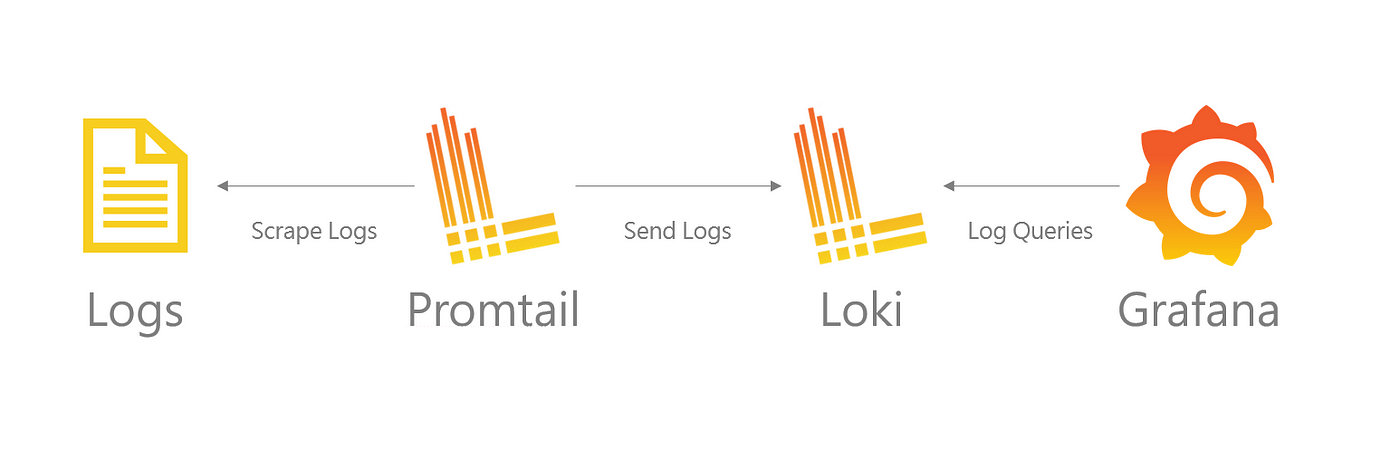
\includegraphics[width=1\textwidth]{./images/loki-promtail.png}
    \caption{Logging architecture.}
    \label{fig:logging_architecture}
\end{figure}

\section{Feature Flag System}
Feature flags are a useful tool for managing software features. They allow system administrators to enable or disable features based on contextual information, such as user roles or location. Feature flags also support A/B testing by enabling controlled rollout, allowing only a subset of users to access a new feature. Additionally, they can be used when integrating a new API into production, allowing testing before deprecating the previous API.

We will not focus on selecting a Feature Flag System. Unleash has provided an objective list of OSS tools that address this need \Parencite{UnleashFeatureFlags}. This is notable, given that Unleash specializes in Feature Flags. It is licensed under the Apache-2.0 license, has 12k stars and 759 forks on GitHub \Parencite{UnleashRepo}, and has been ranked as the top Feature Management Software on G2 \Parencite{UnleashFeatureFlags}. Based on this, we will examine the main features of Unleash rather than other tools. While Unleash offers a more feature-rich enterprise version, the OSS features are sufficient for this project.

\subsection{The Anatomy of Unleash}
Unleash manages feature flags using a client-server architecture. The server controls the feature flags, while the client retrieves and evaluates them via a REST API. The exported endpoints are typically wrapped by a client library, such as the unleash-client-go library for Go, developed by Unleash \Parencite{unleash_client_go_v3}.

Feature flags are organized within projects, which can be used to group related feature flags, teams, or modules. A project can also be assigned per tenant to simulate multi-tenancy. The OSS version supports one project, the Pro version allows up to three, and the Enterprise version supports up to 500 \Parencite{unleash_resource_limits}.

Projects contain environments. The OSS version permits two environments \Parencite{unleash_resource_limits}, which is sufficient for a production environment and an optional development environment if the environments differ. A feature flag is then assigned to an environment. 

\subsection{Activation Strategies}
An activation strategy defines which users receive a feature. It is assigned to a feature flag within an environment. A feature flag can have multiple activation strategies, each evaluated independently. A collection of such reusable activation strategies is called a segment \Parencite{unleash_activation_strategies}.

The default activation strategy is a 100\% gradual rollout, adjustable by setting rollout percentage, targeting, and variants. The rollout percentage determines how many users receive the feature. Targeting specifies which users should be affected, using constraints defined by a context field, an operator, and a value. This allows filtering based on any context. Variants extend a feature flag's payload with additional data to create different versions \Parencite{unleash_activation_strategies}.

\section{Static Website}
Web development involves various technologies and frameworks. Some websites, such as blogs or online CVs, only need to display informational content. In these cases, the Model-View-Controller (MVC) pattern may not be necessary. Instead, static site generators can be used to create static websites. These tools convert plain text files into static HTML pages and are commonly used for blogs, documentation, and content-driven sites.

\subsection{Static Site Generators}
Several static site generators are available, including Jekyll \Parencite{jekyll}, Astro \parencite{astro}, and Hugo \Parencite{hugo}. Each provides templates that allow users to customize their website's appearance. A popular Jekyll theme, Just the Docs \Parencite{just-the-docs}, converts Markdown files into well-formatted HTML pages for online use, making web development more accessible. Documentation should be easy to write; otherwise, it is less likely to be created.

Jekyll, written in Ruby, powers GitHub Pages \Parencite{GitHubPagesJekyll} and organizes content using a simple directory structure. Key folders include \texttt{assets}, \texttt{\_layouts} (for templates), \texttt{\_includes} (for reusable components), \texttt{\_sass} (for styling) and the configuration file \texttt{\_config.yml}. The complete directory structure is available on Jekyll's homepage \Parencite{jekyll}. Content is typically written in Markdown and converted to HTML during the build process. HTML can be directly hardcoded into layouts. The final website consists of static files placed in the \texttt{\_site} folder, which a web server can serve.

\subsection{Web Servers}
Web servers are the backbone of the internet -- they handle requests from users and deliver content like websites, images, and other resources. 

GitHub Pages is a free service to host a static website. It is a great option for hosting documentation, as it is easy to set up and integrates well with GitHub repositories -- it is not even necessary to create a pipeline to deploy the website, as everything is handled by GitHub after enabling the feature. GitHub pages allow one site per repository \Parencite{GitHubPagesLimits}.

NGINX is an HTTP(S) server, reverse proxy, content cache, load balancer, TCP/UDP proxy server, and mail proxy server, distributed under the 2-clause BSD License. It is widely used due to its performance and resource efficiency, making it one of the most deployed web servers and a frequently used Docker image. NGINX also supports multiple Kubernetes Ingress Controllers, including its own \Parencite{NginxWebsite}. 

Using Docker's multi-stage builds, a static website can be created using a single Dockerfile. Earlier stages contain the necessary build tools, while the final image only includes the static files and configuration. This approach optimizes the final Docker image by excluding unnecessary build dependencies, leaving only the NGINX application, its configuration file, and the static HTML files.

\section{Private Registry}\label{sec:private_registry}
A private registry is used to store and manage container images, allowing organizations to host their own images, control access, and track versions. While Docker Hub is a public registry, it also provides private repositories. GitLab and GitHub offer similar repository services. In some cases, hosting a private registry locally is preferable to prevent images from being pushed outside the firewall. This approach can reduce costs associated with hosted registries or ensure images remain airgapped.

Docker Hub introduced new rate limits, setting a maximum of 10 pulls per hour for unauthenticated users and 100 pulls per hour for authenticated users. This was a significant reduction from the previous limits of 200 pulls per six hours for unauthenticated users and 200 pulls per six hours for authenticated users. In response to user feedback, Docker revisited its policies and decided to maintain the current rate limits \Parencite{DockerHubPolicies}.

To address the limitations, that was later called off, local registries can be implemented as pull-through caches for Docker. Two methods for achieving this are using mirrors \Parencite{dockerhubmirror} or a more advanced solution with Harbor \Parencite{harbor}. This makes Docker pull all images from the local private registry, which in turn pulls the images from Docker Hub if unavailable in the pull-through cache.

\subsection{Mirror}
Mirrors are natively supported in Docker but cannot mirror private registries -- only the central Hub can be mirrored \Parencite{dockerhubmirror}. Configuration consists of two steps.

To set up a registry as a pull-through cache, a proxy section must be added to the configuration file. Parameters include \texttt{remoteurl}, \texttt{username}, and \texttt{password}. The \texttt{remoteurl} specifies the URL of the remote registry to mirror, while \texttt{username} and \texttt{password} provide authentication credentials \Parencite{dockerhubmirror}.

To configure the Docker daemon to use a registry mirror, either pass the \texttt{--registry-mirror} option when starting dockerd, or modify \texttt{/etc/docker/\allowbreak daemon.json} to include the registry-mirrors key \Parencite{dockerhubmirror}.

\subsection{Harbor}
Harbor serves a similar function to a mirror while offering additional capabilities. It is a cloud-native registry that stores, signs, and analyzes content. As an open-source project under the Cloud Native Computing Foundation (CNCF), it is licensed under the Apache License 2.0. Harbor includes a web interface for image management, user authentication, and role-based access control (RBAC). It supports security assessments and integrates with CI/CD pipelines \Parencite{harbor}.

Docker must be configured to use the pull-through cache as described above. In Harbor, proxy settings are established by creating a proxy cache project that connects to a target registry via a registry endpoint \Parencite{harbor}.

\section{Containers \& Virtual Machines} \label{sec:vm_vs_container}
Modern infrastructure relies on technologies that package applications and dependencies while keeping them isolated from the system they run on. Containers provide lightweight environments managed by Kubernetes. KubeVirt extends Kubernetes to support virtual machines, allowing traditional workloads to run alongside containers. NixOS offers a reproducible way to build disk images and manage system configurations.

Virtualization allows a single physical resource, such as RAM, CPU, disk, or networking, to be divided into multiple virtual instances. The main difference between them is that virtual machines simulate an entire system, including hardware, while containers virtualize only the software environment above the operating system \Parencite{atlassian_containers_vs_vms}.

\subsection{Containers}
Containers are lightweight software packages that bundle all necessary dependencies to run an application, including system libraries, third-party code, and other operating system components. They allow quick modifications and iteration, with most container runtime systems providing public repositories of pre-configured containers. These repositories offer access to widely used applications like databases and messaging systems, reducing setup time and simplifying deployment \Parencite{atlassian_containers_vs_vms}.

Shared host exploits may occur because containers share the same underlying hardware below the operating system layer. A vulnerability in one container could allow unauthorized access to the host system, affecting other containers running on the same infrastructure. Public repositories of pre-built containers also introduce risks, as images may contain exploits or be compromised \Parencite{atlassian_containers_vs_vms}.

\subsection{Virtual Machines}
Virtual machines are software packages that emulate low-level hardware components such as CPU, disk, and networking devices. They may also include a software stack to operate on the emulated hardware, creating a fully functional computational system snapshot \Parencite{atlassian_containers_vs_vms}.

Virtual machines provide full isolation security, running as standalone systems. This prevents exploits from spreading between virtual machines on a shared host, ensuring that a compromised machine remains contained. They also support interactive development, allowing manual installation of software and the creation of snapshots to preserve specific configurations. These snapshots can be used to restore a virtual machine to a previous state or deploy additional instances with identical setups \Parencite{atlassian_containers_vs_vms}.

Despite these advantages, virtual machines have limitations. Iteration speed is slower since each snapshot represents an entire system, requiring significant time to regenerate and validate modifications. Additionally, storage size cost can be high, as virtual machines often occupy several gigabytes of disk space, potentially leading to storage constraints on the host system \Parencite{atlassian_containers_vs_vms}.

\subsection{KubeVirt}
KubeVirt is an open-source virtualization API extension for Kubernetes, licensed under the Apache License 2.0 \Parencite{kubevirt_license} and maintained as a Cloud Native Computing Foundation (CNCF) project \parencite{kubevirt_cncf}. It enables the management of virtual machines alongside containers by introducing custom resource definitions (CRDs), which extend Kubernetes to support VM workloads using its native tools. This allows users to run both containerized and virtualized applications within the same cluster, creating a unified infrastructure for diverse workloads.

KubeVirt uses a Docker image based on \texttt{scratch}, where the container disk image, QCOW2, is stored in the \texttt{/disk} directory. QCOW2 is recommended as it reduces image size. The image contains only the disk with no additional content \Parencite{kubevirt_disks_volumes}.

KubeVirt consists of three main cluster components: \texttt{virt-api}, \texttt{virt-\allowbreak controller}, and \texttt{virt-operator}. The \texttt{virt-controller} manages the lifecycle of VMs, while the \texttt{virt-operator} ensures that KubeVirt components are correctly deployed and functioning. The \texttt{virt-api} provides a RESTful interface for interacting with KubeVirt and managing VM resources.

Each virtual machine instance (VMI) is associated with a pod that contains \texttt{virt-launcher}, \texttt{libvirtd}, and \texttt{qemu}. However, the VMI itself does not run within the pod \Parencite{kubevirt_architecture}. Instead, it operates directly on the host as its own instance type: \texttt{virtualmachineinstance.kubevirt.io}. The \texttt{virt-\allowbreak launcher} is responsible for spawning the VM on the host.

If hardware virtualization is unavailable, software emulation can be used instead \Parencite{kubevirt_installation}. In this mode, virtualization is handled entirely by software rather than relying on CPU extensions. Software emulation is expectedly less efficient than hardware virtualization.

\subsection{NixOS Disk Images}
NixOS is a declarative operating system that defines system configurations, including installed packages, services, and settings.

It can build Copy-On-Write version 2 (QCOW2) disk images for virtual machines \Parencite{nixos_vm_configuration}. Using a Nix expression, users generate a QCOW2 image with a predefined environment, ensuring consistency and eliminating manual setup \Parencite{nix_language_tutorial}.

NixOS configurations can be tested in virtual machines without installation on physical hardware. Unlike interactive configuration, which lacks documentation, NixOS provides a structured approach. Interactive setups make modifications difficult and do not track changes, leading to uncertainty about the image's contents.

This approach allows image generation at runtime instead of storing large QCOW2 images. Since they cannot be stored in Git due to their size, declarative configuration enables automated, reproducible builds when needed.

\section{Static Code Analysis}
Static code analysis is a software testing technique that examines code without executing it, serving as the counterpart to dynamic code analysis. It is used to identify potential vulnerabilities, bugs and code smells. Static code analysis can be performed manually or automatically using tools. The latter is more efficient and less error-prone, as it can be integrated into the development process.

In this section we will cover the tools used in this project for static code analysis. These tools include Dependabot, SonarCloud, and Linting.

\subsection{Dependabot}
Dependabot is a dependency management tool rather than a static code analysis tool. It is included in discussions of repository scanning because it identifies outdated dependencies, checks for updates, and creates pull requests to keep them current. It also provides security alerts for known vulnerabilities in dependencies, helping developers address risks promptly. Dependabot supports package managers such as pip, npm, and Maven and can be configured to check for updates on a schedule \Parencite{GitHubDependabotVersion2025}.

\subsection{SonarCloud}
SonarCloud is a cloud-based platform for continuous code quality and security inspection. It performs static code analysis to detect bugs, vulnerabilities, and code smells, supporting multiple programming languages. Integrated seamlessly with CI/CD pipelines, it enables automated code quality checks throughout development \Parencite{SonarQubeDocs2025}.

The service offers a web interface for monitoring quality metrics and trends over time. It is free for public repositories; however, private repositories require a paid subscription \Parencite{SonarCloudPricing2025}. In contrast, SonarQube is a self-hosted solution, licensed under the GNU Lesser General Public License v3.0 \Parencite{SonarQubeLicense2025}. It provides similar functionality and supports private repositories -- while the Community Edition is free, advanced plans come at a cost.

\subsection{Linting}
Linting is a static code analysis technique used to detect errors, enforce coding standards, and improve code readability. Some linters assess cyclomatic complexity, helping developers understand the maintainability of their code. By identifying issues early in the development process, linting ensures consistency and enhances code quality. Linting tools can be integrated into IDEs or run as part of the build process \Parencite{SuperLinter2025}. Popular options include ESLint for JavaScript, Pylint for Python, and SonarQube for IDE (formerly SonarLint), which supports multiple programming languages.

SonarQube for IDE integrates automated code review into your development environment \Parencite{SonarQubeConnectedMode2025}. Connected mode links projects to SonarQube Cloud or Server, ensuring consistent best practices, preventing security vulnerabilities, and reducing technical debt before code is committed.

\section{Henrik Thesis}\label{sec:henrik_thesis}
Since Henrik's thesis is not publicly accessible, we cannot reference it directly. Instead, we provide a summary of its key points.

Henrik's thesis investigates the design and deployment of CTF challenges, with a focus on simplifying integration and improving the security and flexibility of hosting environments. The work begins with a comprehensive review of current open-source Jeopardy-style CTF platforms, including CTFd, Haaukins, rCTF, and kCTF, analyzing their strengths and limitations in areas such as challenge isolation, continuous integration and developer usability. 

Common challenges include difficulty testing challenges outside the host environment and insufficient container isolation, which could allow attackers to compromise the underlying system.

To address these issues, the thesis presents a proof-of-concept CTF platform that enables:

\begin{itemize}
    \item On-demand challenge deployment in isolated virtual machines (VMs), mitigating container escape risks.
    \item Use of Docker Compose files for both local development and remote deployment, easing the development workflow.
    \item Automated and manual testing of challenges via an API, without requiring administrative access.
\end{itemize}

The system integrates Kubernetes and KubeVirt for orchestrating VMs, and extends the popular CTFd frontend with support for managing dynamic, containerized challenges. Although VM-based deployment introduces startup latency and higher memory usage compared to container-only solutions, it significantly improves security through stronger isolation.

In conclusion, the thesis contributes a deployable platform prototype, empirical performance evaluation, and architectural guidance for future CTF systems, particularly those emphasizing safe, developer-friendly challenge integration.

\chapter{Implementation}\label{chap:implementation}
This chapter outlines the implementation of a scalable, secure, and fault-tolerant CTF platform, building on prior concepts and technologies. The MVP is considered complete when the platform supports multiple users who can create, manage, and participate in challenges. Additionally, it must provide documentation for users, administrative monitoring, and robust security measures, including encrypted access and fault tolerance.

\section{Architecture}\label{sec:architecture}
The architecture of the CTF platform is designed to be modular and extensible, allowing for easy integration of new features and services. The platform is built on a microservice architecture, with each service responsible for a specific functionality. This approach enables independent development, deployment, and scaling of services, ensuring that the platform can adapt to changing requirements and user needs.

UCloud was never selected for its capabilities but for its affordability. While the availability of UCloud resources through the university was an advantage, the challenges of building a usable and widely accessible platform remained significant -- though solving them was an engaging task. This section first presents the architecture as it was successfully implemented on UCloud before detailing its final deployment on GCP. Although GCP is an expensive option, it was the only one investigated that provides hardware virtualization, a required capability for the platform.

\subsection{Services}

Figure \ref{fig:architecture} illustrates the UCloud architecture. Network limitations posed a significant challenge, which was mitigated by implementing a Headscale network overlay and integrating a GCP VM. The GCP VM served as the entry point and login server for the Headscale network. All nodes, including GCP itself, are connected through this login server using Tailscale, enabling communication across nodes without the usual network restrictions. Tailscale is a VPN based on WireGuard \Parencite{TailscaleDocs}, while Headscale is a self-hosted alternative to Tailscale's coordination server \Parencite{TailscaleOpenSource}. 

\begin{figure}[h]
    \centering
    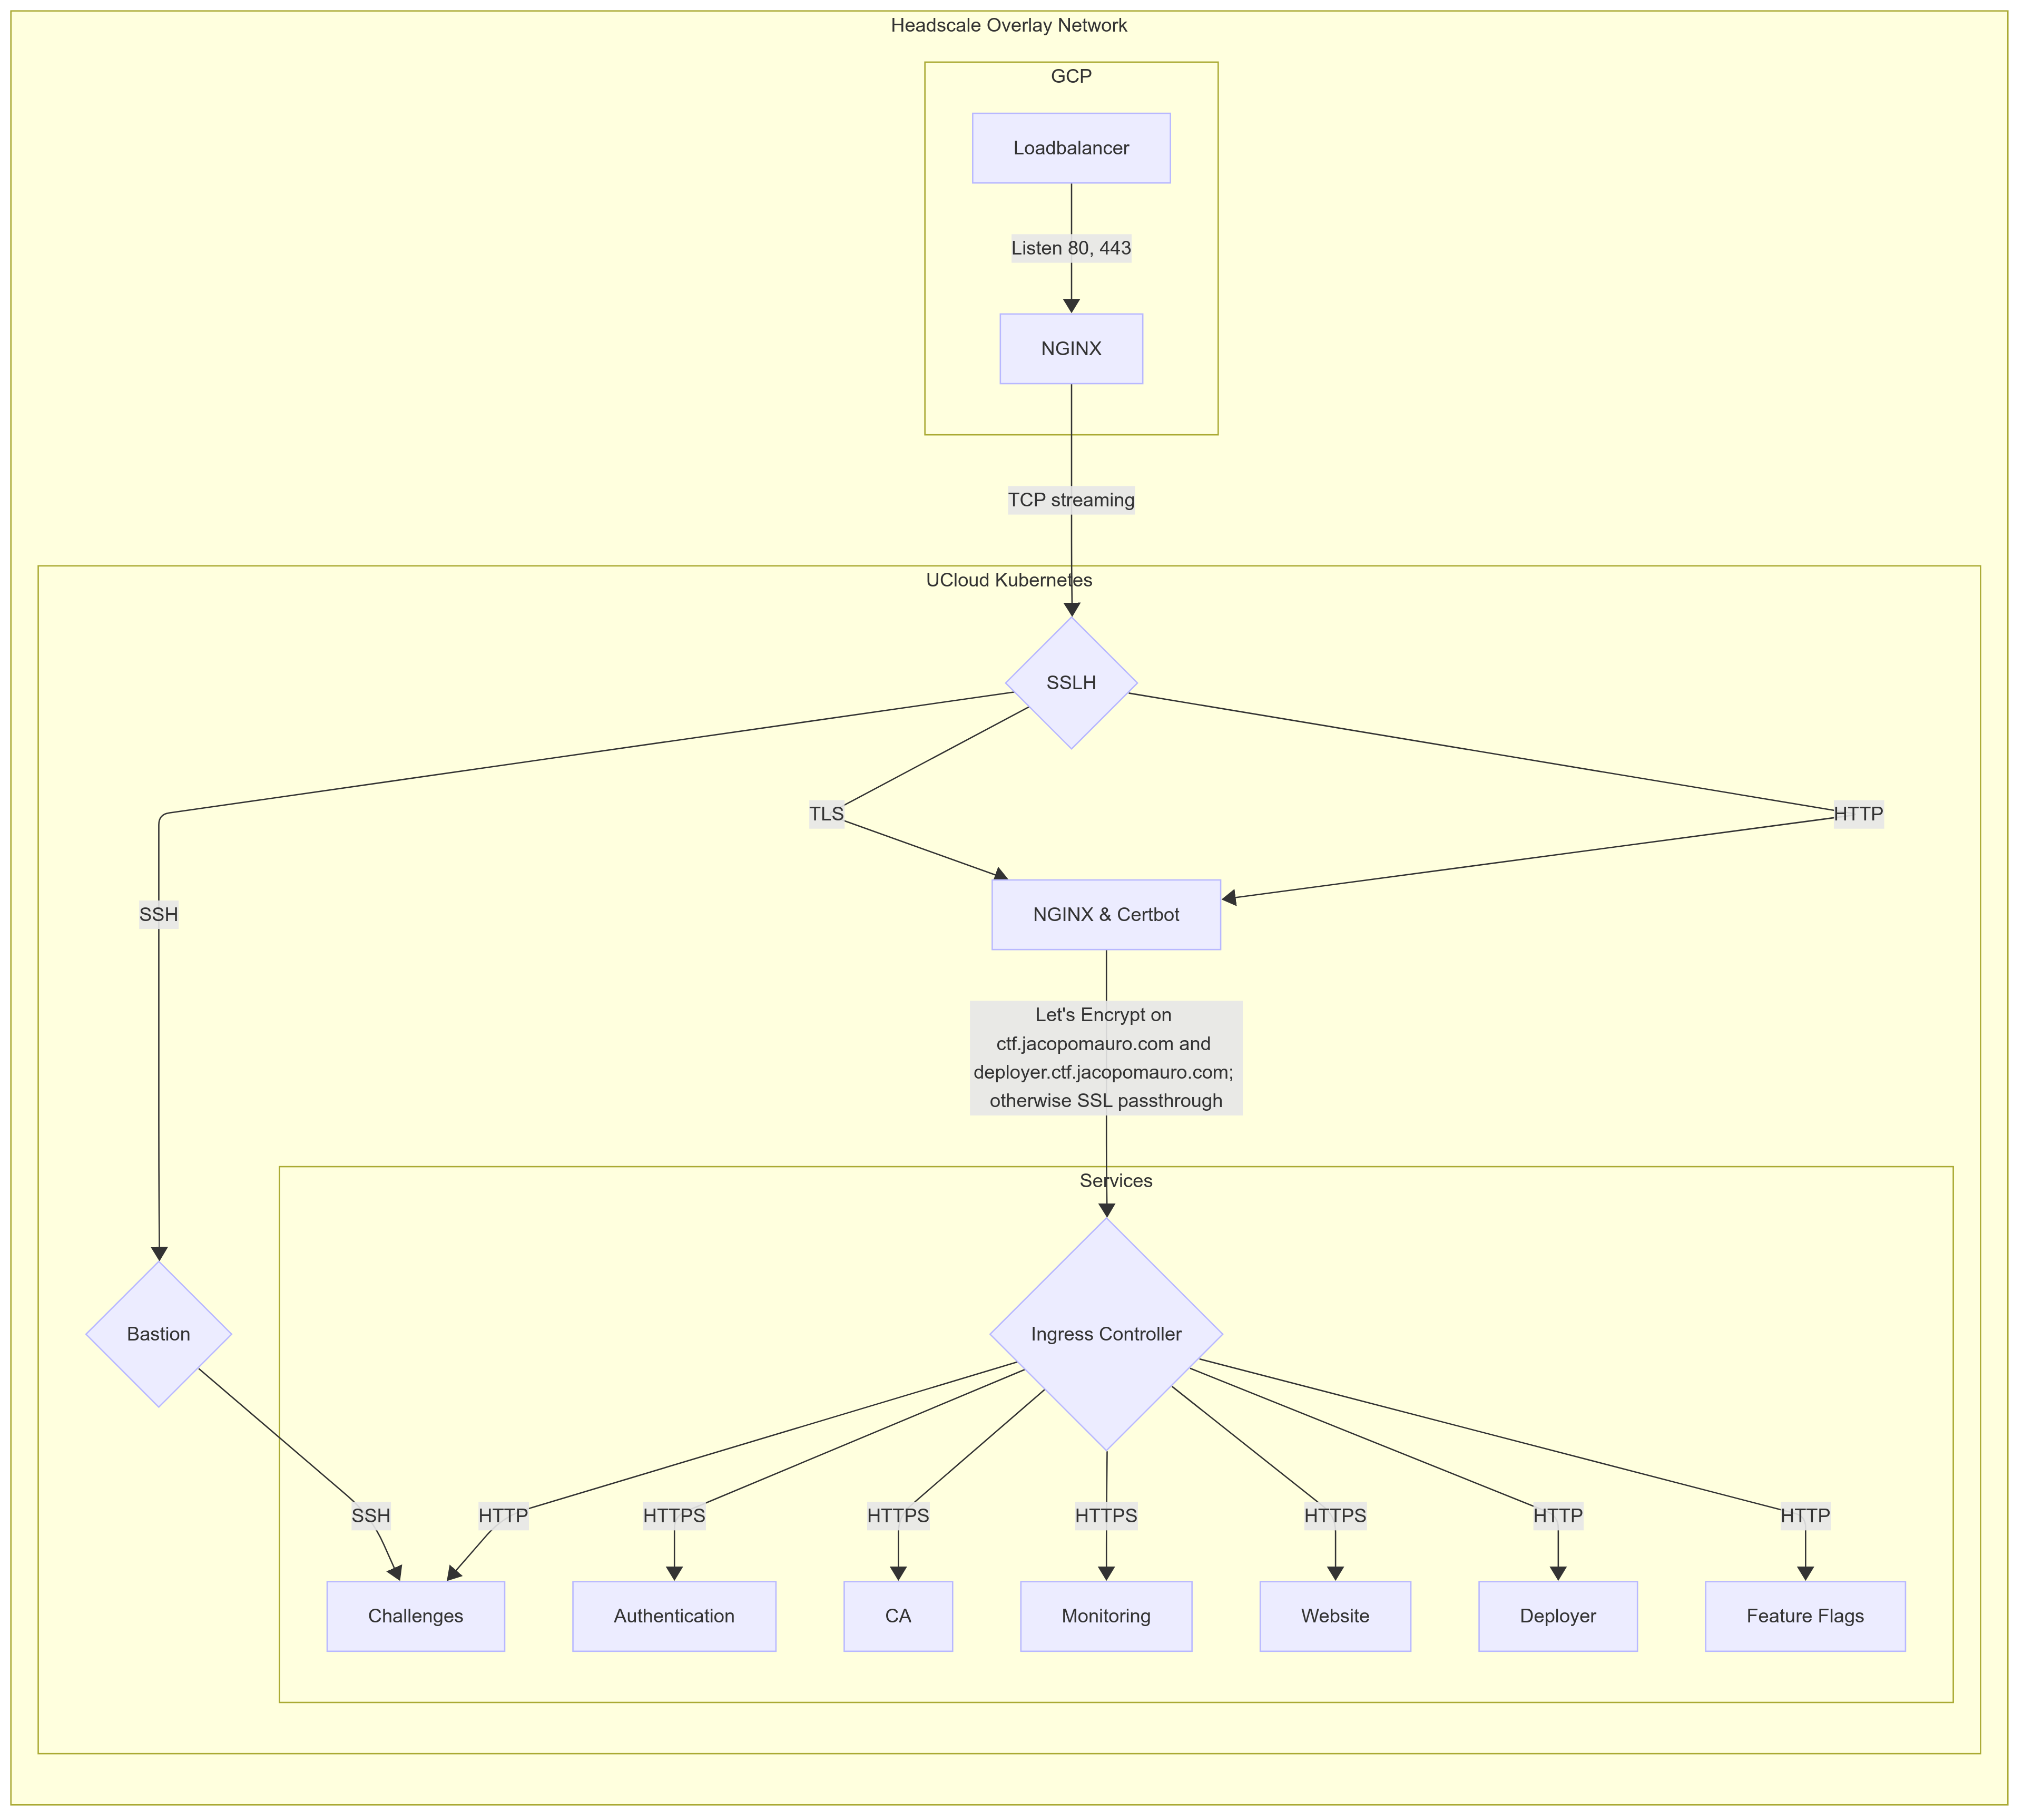
\includegraphics[width=1\textwidth]{images/ucloud-architecture.png}
    \caption{Architecture of the CTF platform deployed on UCloud.}
    \label{fig:architecture}
\end{figure}

The NGINX instance on GCP facilitates TCP streaming to UCloud, as this approach proves optimal for the Bastion. Initially, GCP was only used as a login server, since SDU offered a domain name for free. The domain name had to point to a UCloud VM and was linked to a proxy that applied the certificate and forwarded requests to the UCloud server. While the wildcard certificate was useful, handling TLS termination at the cluster level was preferred.

SSLH is a protocol multiplexer that routes traffic to different services based on the detected protocol. It is used to direct SSH traffic to the Bastion while forwarding HTTP(S) traffic to the NGINX/Certbot proxy. This setup prevents SSH traffic from reaching the proxy, which is unable to handle it, and ensures that no certificates are applied to SSH connections, avoiding the need for users to tunnel SSH via TLS.

The trusted TLS certificate could have been managed at the ingress controller instead of the Certbot proxy. This approach was chosen because it simplifies the setup, allowing all internal services to use certificates issued by our own PKI. Rather than modifying this configuration for production deployment, adding a proxy in front of the system to handle TLS termination makes the adjustment more straightforward.

The remaining architectural details will be covered in their respective sections, as they pertain to platform functionality rather than system architecture. The \textit{services} box in Figure \ref{fig:architecture} represents the core components of the platform, while all other elements ensure secure access to these services for users.

Migrating this architecture to GCP simplifies the setup significantly. In fact, everything outside the UCloud Kubernetes box in Figure \ref{fig:architecture} can be removed. With this change, SSLH serves as the new entry point, eliminating both the network overlay and the additional proxy forward. Be aware that SSLH cannot be exposed on a privileged port. Something needs to redirect traffic from port 80 and 443 to SSLH.

\subsection{Storage}

We recognize that building a completely fail-safe system is unrealistic; instead, our priority is to create a safe-to-fail system. When shit hits the fan, a full redeployment of the platform may be necessary. In such cases, minimizing downtime is crucial, but protecting data integrity is non-negotiable. To eliminate this risk, we have opted for object storage buckets in MinIO, ensuring robust and reliable data management. The setup is illustrated in Figure \ref{fig:storage-provisioning}.

\begin{figure}[h]
    \centering
    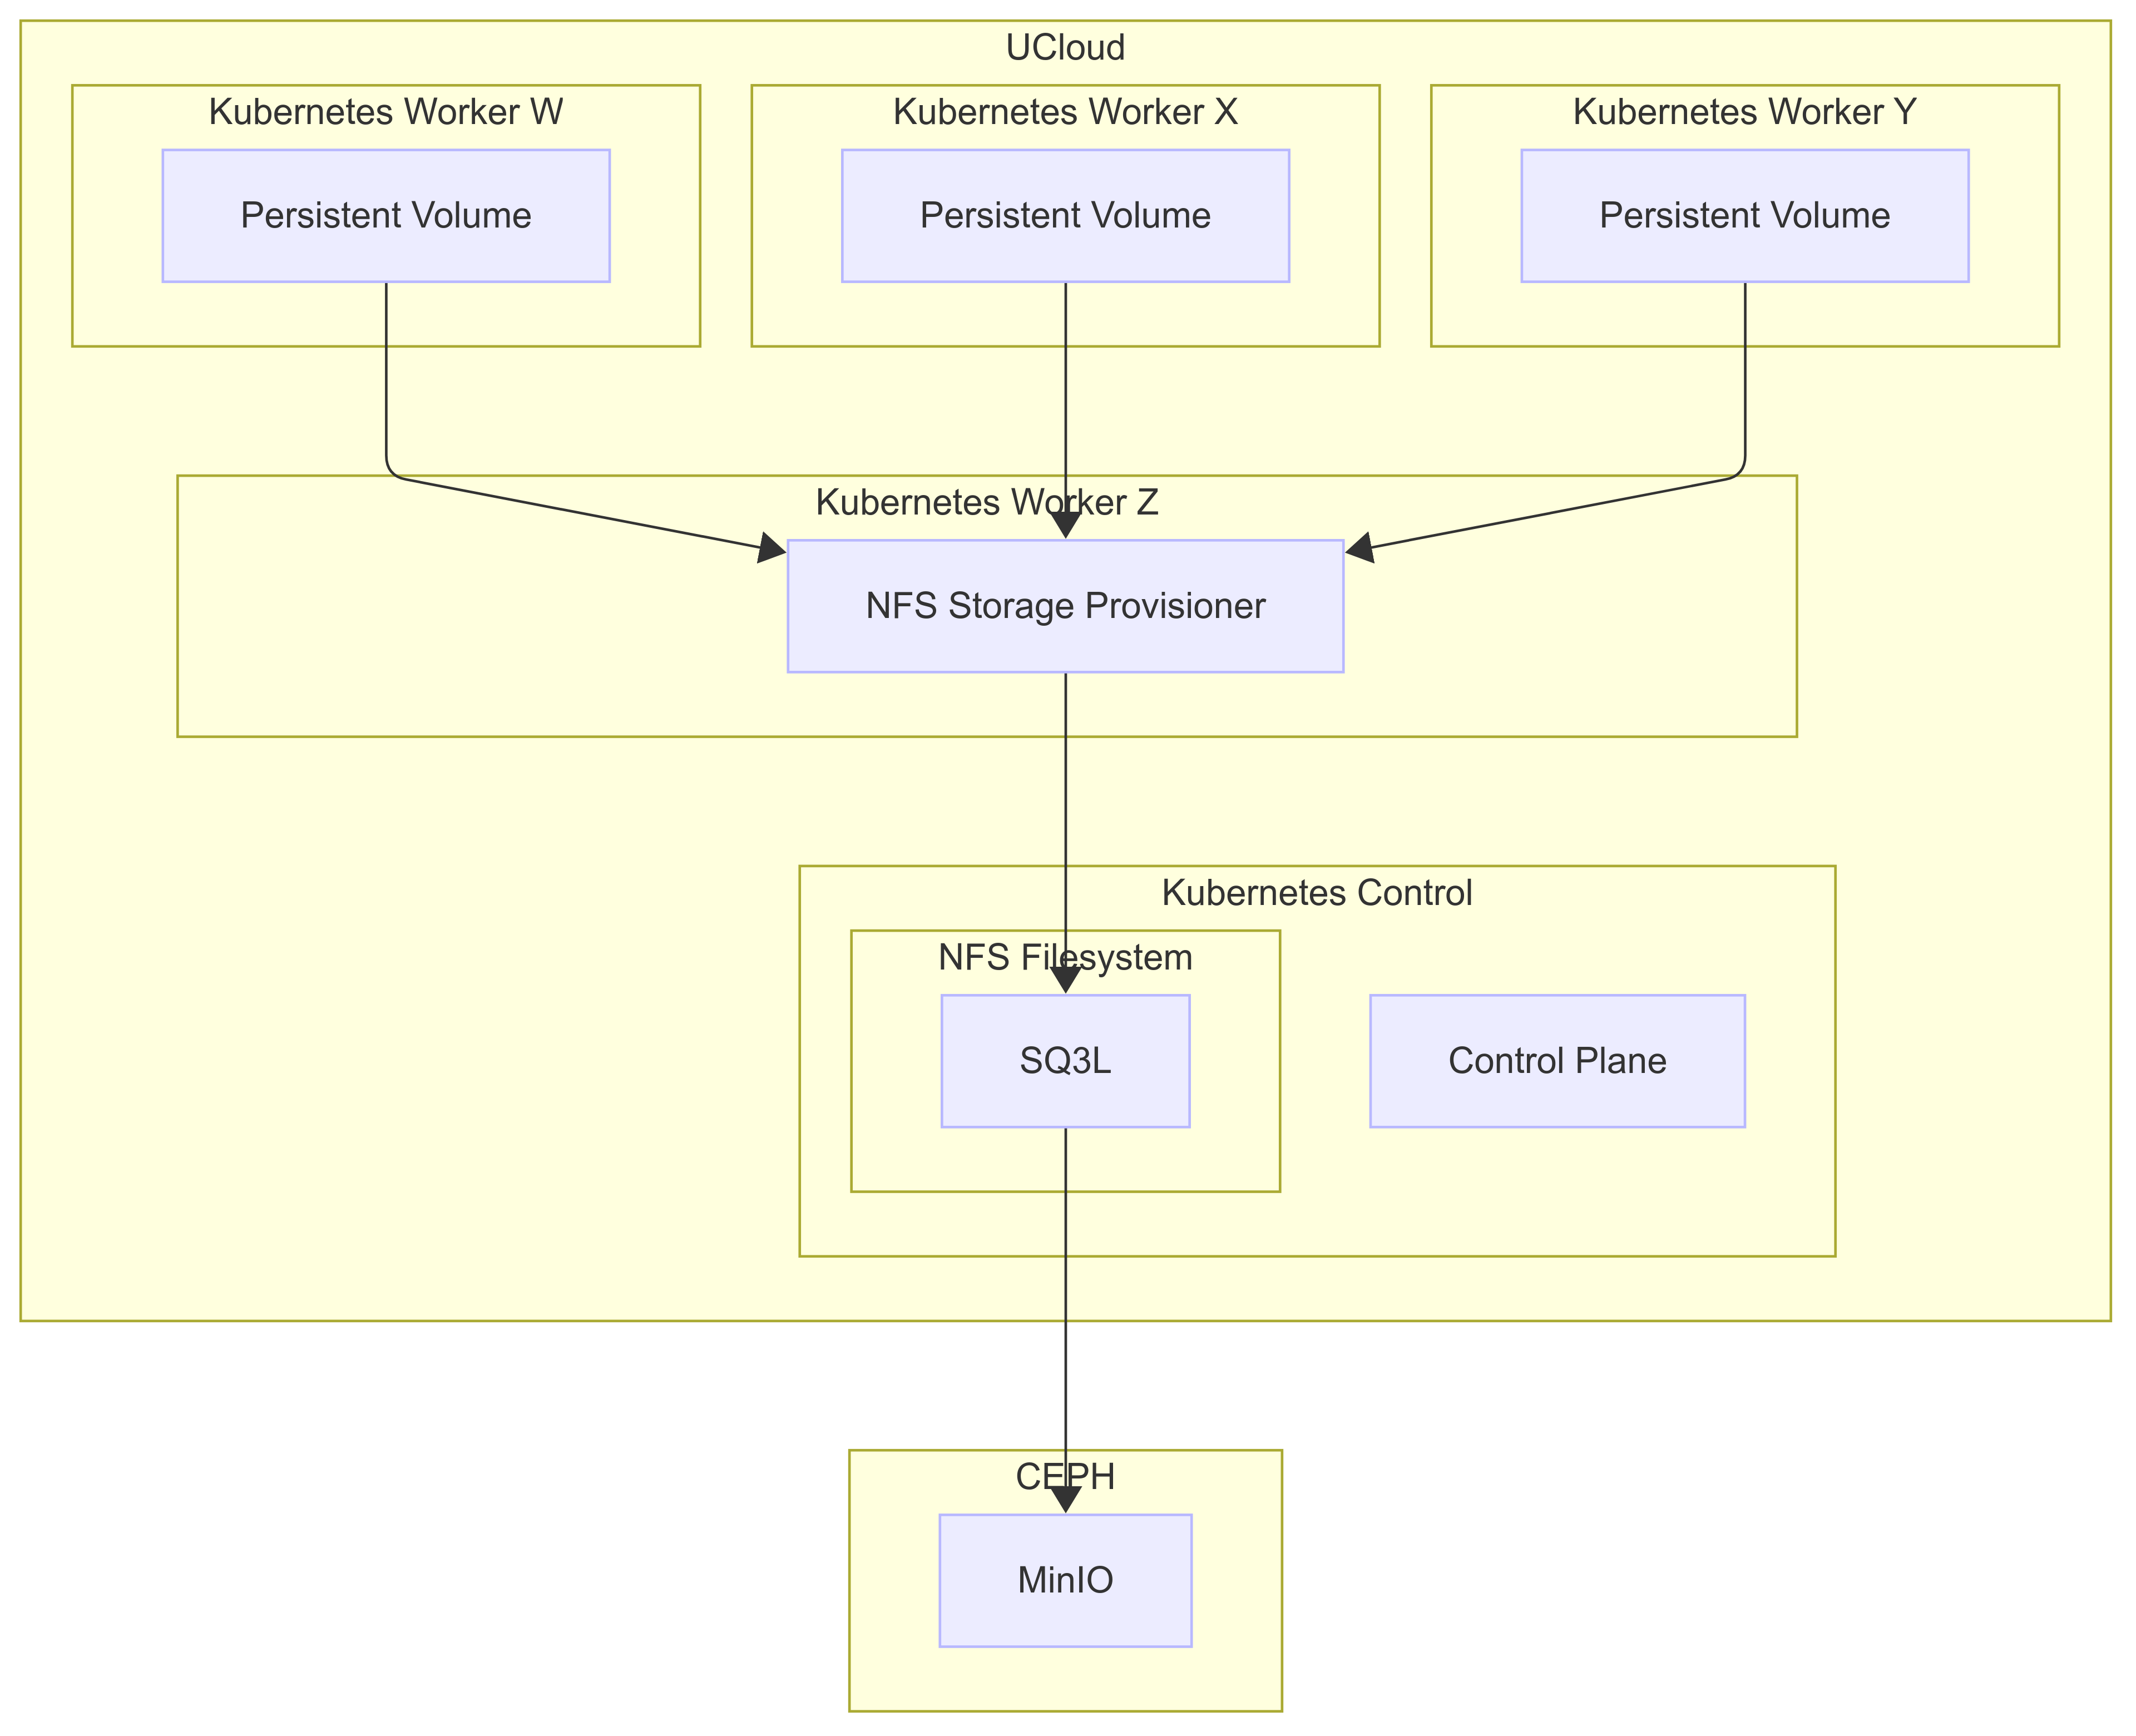
\includegraphics[width=1\textwidth]{images/storage-provisioner.png}
    \caption{Storage provisioning architecture of the CTF platform on UCloud using MinIO.}
    \label{fig:storage-provisioning}
\end{figure}

The architecture initially relied on the Rancher Local Path Provisioner, configured as a shared filesystem using the \texttt{hostPath} volume type to store data on a specified path on the host. As retaining data across VM restarts became a necessity, we introduced MinIO as an object storage solution \Parencite{miniosdu}. To integrate MinIO, we first adopted S3FS, a FUSE-based filesystem, but it lacked support for certain filesystem operations, causing databases to crash when interacting with it \Parencite{s3fsrepo}. To resolve this, we replaced S3FS with S3QL, another FUSE-based filesystem that provides full filesystem functionality \Parencite{s3qlrepo}. However, S3QL could not be mounted on multiple nodes simultaneously \Parencite{s3qlfaq} -- a critical requirement for the current setup. To address this limitation, we transitioned from the Local Path Provisioner to an NFS storage provisioner, consolidating all storage within a single folder on the control node, where S3QL is mounted on the same path as MinIO, allowing MinIO to provide block storage while S3QL handles filesystem operations.

The NFS provisioner provides the same benefits as a shared filesystem: pods are not restricted to the same node as the storage, allowing them to be scheduled on the least-loaded node -- even after restarts.

Migrating this architecture to GCP introduces minimal changes. Instead of using MinIO, we leverage GCP's persistent disks for storage, while the rest of the architecture remains unchanged.

\section{Pulumi}
Pulumi's ability to use Terraform providers makes it well-suited for managing the entire infrastructure. However, Terraform was introduced in this project primarily due to existing expertise within the team. The author of this thesis works with Pulumi, while Matteo Trentin manages Terraform -- this division is based on individual proficiency. While the goal is to maintain a simple technology stack, compromises are necessary in a team environment with tight deadlines. If needed, this setup can be adjusted in the future. This thesis focuses on Pulumi, as the Terraform IaC was not developed by the author.

\subsection{Projects \& Stacks}
When starting a new project, it is essential to determine how to organize the Pulumi project and its stacks. To assist in this decision, the Pulumi documentation provides insights into the trade-offs between different approaches \Parencite{pulumiProjects2025}.

The monolithic approach is well-suited for projects that prioritize simplicity, version control, and agility. This method makes it easier to track dependencies, configure package managers, and manage code efficiently, as everything can be previewed and handled in a unified manner.

The micro-stacks approach, similar to microservices but applied to projects and stacks, offers greater independence. Each stack can be deployed separately, making it ideal for projects with varying deployment cadences. Security is another key factor. Large organizations often require Role-Based Access Control (RBAC), which makes micro-stacks advantageous. This approach enables fine-grained access control, ensuring that critical infrastructure can only be modified by selected team members.

For this project, a hybrid approach was adopted. While it primarily relies on micro-stacks, keeping related components together, it also incorporates monolithic elements since the stacks are not entirely independent. The stack organization follows a layered structure. The base layer includes essential components like Custom Resource Definitions (CRDs), secret generation, storage provisioner, KubeVirt, namespaces, and the ingress controller. Directly above this is the PKI, responsible for certificate issuance. 

The remaining stacks exist on the same hierarchical level. The Monitoring stack is completely independent, collecting metrics and logs from the Kubernetes cluster in a passive, non-intrusive manner. Monolithic traits arise in the Application stack, as it combines various unrelated services. While the authentication stack is independent, certificates depend on it for issuing personal SSH certificates, creating a circular dependency (explained in Section \ref{sec:smallstep}).

High coherence and low coupling are vital for effective stack design. While it is important to group only related elements together, the decision to create new stacks should align with the project's scope and complexity. For smaller projects, maintaining simplicity is often more practical. The stack relationships are visually represented in Figure \ref{fig:pulumi_stacks}.

\begin{figure}[h]
    \centering
    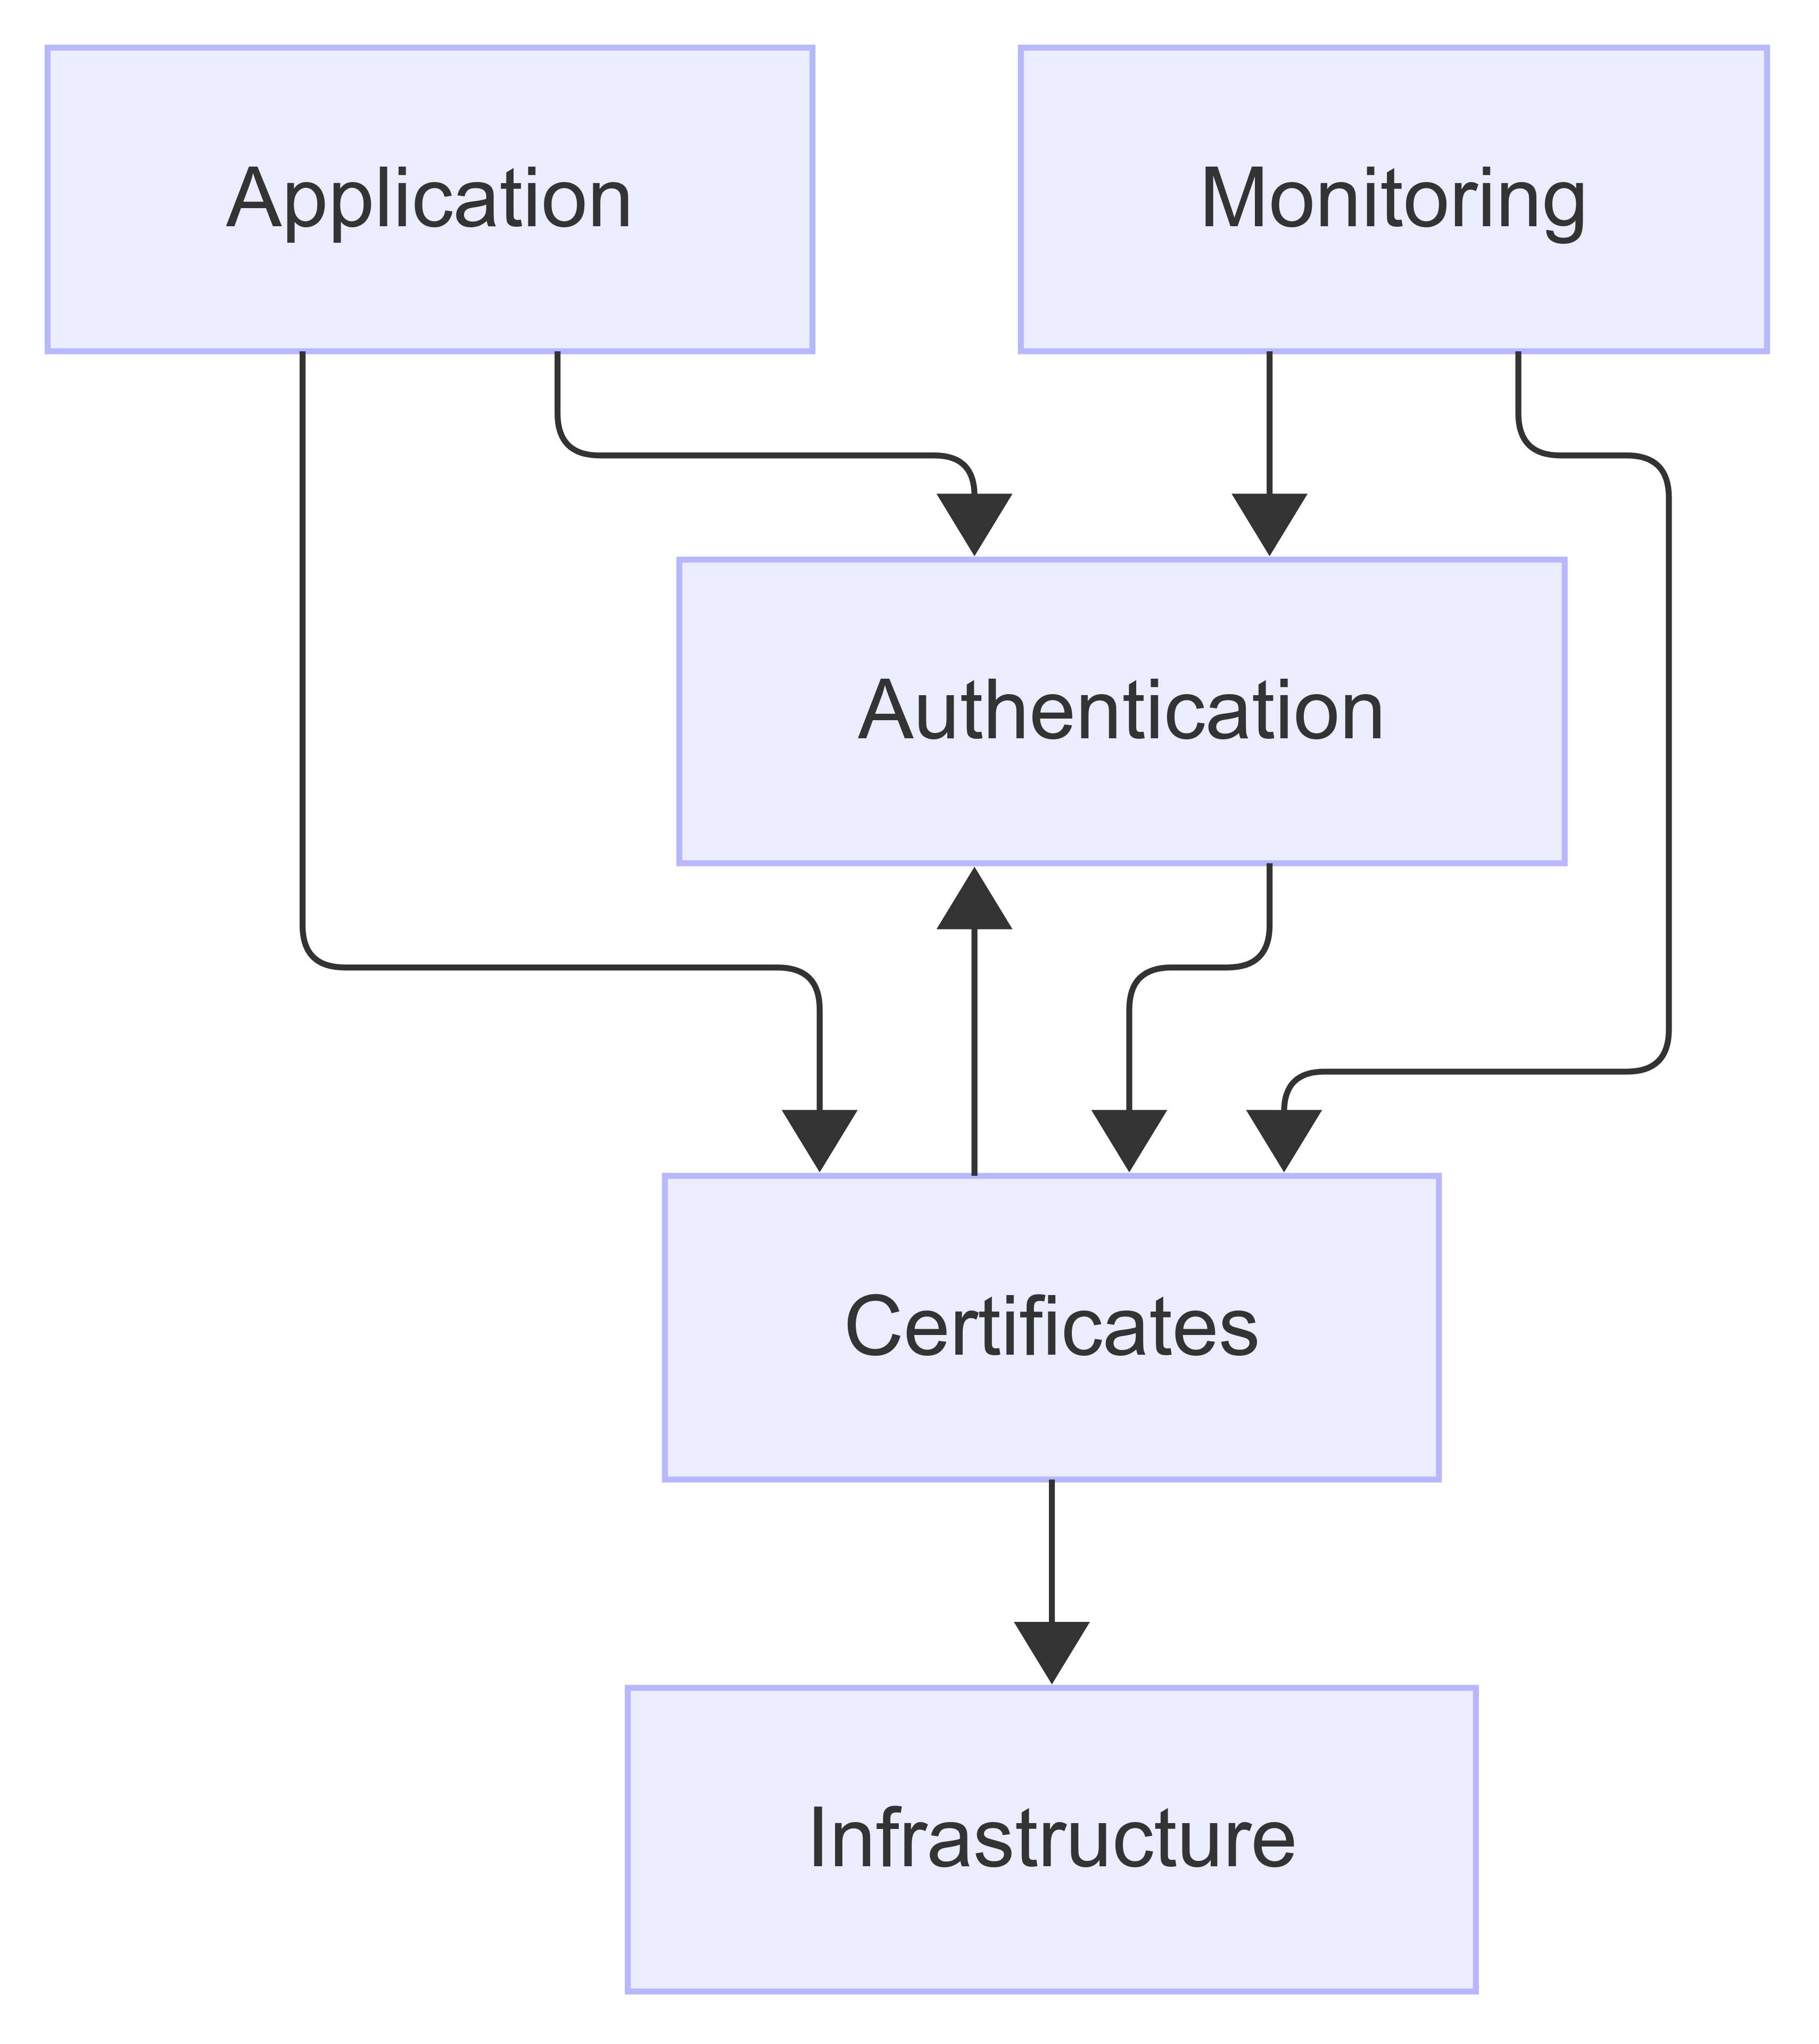
\includegraphics[width=.45\textwidth]{images/pulumi_stacks.png}
    \caption{Pulumi Stacks Relationship. An arrow pointing from a source to a target indicates that the source depends on the target. Given the layered approach, these relationships are transitive. However, arrows targeting certificates are explicitly included due to their significance.}
    \label{fig:pulumi_stacks}
\end{figure}

Our project consists of five Pulumi projects, each with a specific role to play:

\begin{itemize}
    \item \textbf{Application:} Home to CTF platform/cloud-specific functionality.
    \begin{itemize}
        \item \textbf{Homepage:} A user guide for navigating and utilizing the platform.
        \item \textbf{SSHD Alpine bastion:} A secure SSHD server based on Alpine Linux, serving as a bastion host for your cloud environment.
        \item \textbf{CTFd:} A CTF platform for hosting cybersecurity challenges and competitions.
        \item \textbf{Deployer Backend:} The backend service providing core functionality and APIs for the platform.
        \item \textbf{SSLH protocol multiplexer:} A protocol multiplexer that allows multiple services to share a single port, such as SSH and HTTPS.
        \item \textbf{NGINX Proxies:} Proxies to upgrade connection and/or move SSL termination to pod.
        \item \textbf{Unleash:} An open-source solution for feature flagging.
        \item \textbf{Reflector:} A Kubernetes utility that automatically mirror secrets across namespaces.
        \item \textbf{Docker Registry:} A system for storing and sharing Docker images.
    \end{itemize}
    \item \textbf{Monitoring:} Ensures cluster observability and log collection.
    \begin{itemize}
        \item \textbf{Prometheus:} A monitoring system and time-series database for capturing metrics and alerts.
        \item \textbf{Prometheus-Operator:} Simplifies the setup and management of Prometheus instances within Kubernetes.
        \item \textbf{Grafana:} An open-source platform for monitoring and observability, providing dashboards and visualizations for your metrics.
        \item \textbf{Loki:} A log aggregation system designed for efficiency and ease of use, seamlessly integrating with Prometheus.
        \item \textbf{Promtail:} An agent that ships the contents of local logs to a Loki instance.
        \item \textbf{Node-exporter:} Exports hardware and OS metrics exposed by Linux kernels for monitoring.
    \end{itemize}
    \item \textbf{Authentication:} Manages SSO capabilities provided by Keycloak.
    \begin{itemize}
        \item \textbf{Keycloak:} An open-source identity and access management solution for SSO, enabling secure authentication and authorization.
    \end{itemize}
    \item \textbf{Certificates:} Handles certificate CA and issuers.
    \begin{itemize}
        \item \textbf{Step Certificates:} A CA toolkit for managing and issuing certificates within your environment.
        \item \textbf{Step Autocert:} Automates the issuance and renewal of TLS certificates to ensure your services remain secure.
        \item \textbf{Step Issuer:} An issuer that integrates with Cert-Manager to manage certificate lifecycles.
        \item \textbf{Cert-Manager:} A Kubernetes add-on to automate the management and issuance of TLS certificates from various issuing sources.
    \end{itemize}
    \item \textbf{Infrastructure:} Takes care of basic cluster configuration.
    \begin{itemize}
        \item \textbf{NFS Storage Provisioner:} Manages dynamic storage provisioning for Kubernetes using NFS, enabling shared storage across nodes.
        \item \textbf{Nginx Ingress Controller:} Manages external access to services in a Kubernetes cluster through HTTP and HTTPS.
        \item \textbf{KubeVirt:} Extends Kubernetes by adding support for running virtual machine workloads alongside container workloads.
    \end{itemize}
\end{itemize}

These are the core services of the platform. Some provide direct user-facing functionality, while others support essential technical operations. Additionally, the platform includes sidecar containers, which are not listed here.

\subsection{Managing Secrets}
Pulumi includes a built-in mechanism for managing secrets. The user provides a passphrase, which is combined with the encryption salt stored in each stack to encrypt secrets. However, these stacks can also include configuration values in plain text. Secrets can be added using the following command:

\begin{minted}{bash}
    pulumi config set --stack <stack> --secret <key> <value>
\end{minted}

And configuration values can be added using the following command:

\begin{minted}{bash}
    pulumi config set --stack <stack> <key> <value>
\end{minted}

This mechanism functions similarly to a password vault, where all secrets are safeguarded by a single master passphrase. As such, it is crucial to ensure that this passphrase is never compromised. While passwords within the stack can be rotated, the passphrase represents a single point of failure.

In case the passphrase have been compromised, it can be updated using the command:

\begin{minted}{bash}
    pulumi stack change-secrets-provider passphrase --stack <stack>
\end{minted}

Only passwords that must be explicitly known, such as Keycloak login credentials, are stored within the stacks. Passwords that only need to be used by the system are generated during deployment. For example, knowing the database password provides no benefit since it is solely used by the application. Similarly, client credentials for OAuth2 clients are designed to remain confidential. By ensuring that these passwords are not accessible, the risk of them being leaked is eliminated, at least to some extent -- any application can be compromised from within.

Generating secrets during deployment ensures fresh credentials with each update but introduces challenges in password rotation. The current implementation generates most passwords at deployment, simplifying initial setup but causing issues for components that rely on persistent credentials, particularly databases that retain old passwords tied to user accounts. If passwords are sourced from the state file, stack updates would not generate new credentials, preventing automatic password rotation. Conversely, enabling password rotation requires migration steps to avoid authentication failures. This suggests that dynamically generating secrets may not always be ideal. Hardcoding secrets directly in the Pulumi stack offers a predictable and controlled approach but increases the risk of exposure. Choosing between these methods requires careful consideration of security, operational needs, and long-term maintainability.

In a monolithic stack, all information is already available within the same stack. When using a micro-stack architecture, it may be necessary to share information between stacks. Stack references make this possible by allowing one stack to access outputs from another, such as randomly generated secrets, or other stack-specific data. This enables generating all secrets in the Infrastructure stack and exporting them to the services that need them.

\subsection{Helm Charts}\label{sec:helm_crds}
Pulumi offers two approaches for deploying Helm charts: as a \texttt{Chart} \Parencite{PulumiHelmChart} or a \texttt{Release} \Parencite{PulumiHelmRelease}. The key difference lies in how Pulumi manages these resources. When using \texttt{Chart}, Pulumi treats all resources within the chart as its own, incorporating them into its state. Conversely, the \texttt{Release} option deploys the Helm chart as a release, meaning the resources are not tracked in Pulumi's state and are managed independently. This approach is useful for charts intended to be managed outside of Pulumi or when keeping the Helm release separate from a Pulumi stack.

One important consideration is that Helm hooks are no longer supported in Pulumi Charts v4. While Chart v3 also lacked hook support, it historically emitted hooks as ordinary child resources. Another notable improvement in Chart v4 is enhanced resource ordering \Parencite{PulumiKubernetesChartV4}. For example, in Chart v3, deploying \texttt{kube-prometheus-stack} was problematic because services dependent on CRDs were created before the CRDs themselves were available. This required manually installing the CRDs within the Infrastructure stack. Chart v4 eliminates this workaround by handling resource ordering automatically. However, the CRDs remain in the Infrastructure stack for flexibility, ensuring availability for other stacks beyond Monitoring -- \texttt{ServiceMonitors}, for example, are widely used across different stacks.

Why use Helm charts at all? The primary advantage is their active community maintenance, which ensures regular updates and improvements. Helm charts bundle numerous resources, reducing the complexity of manually defining and managing them. They provide a streamlined, efficient way to configure and deploy applications compared to writing everything from scratch. Given these benefits, we will rely on Helm charts in this project whenever possible.

In conclusion, Helm charts are preferred over manual resource definitions, and Pulumi Charts v4 will be used to manage their deployment.

\section{Ansible}
Terraform is used to provision the servers. However, since UCloud does not provide a Terraform provider, an alternative approach was required for deploying Kubernetes resources. To address this, we leveraged Ansible -- an agentless automation tool that uses SSH to connect to servers and execute commands remotely, eliminating the need for software installation on target machines.

The majority of the Ansible work has been completed by Matteo Trentin, though I have contributed to specific aspects outlined in this section. My primary contributions include deploying Pulumi stacks, configuring the NFS server, making sure that \texttt{Kubectl} used the Tailscale subnet\footnote{Only needed when deployed on UCloud.}, and developing a deep understanding of the existing Ansible playbooks and roles.

\subsection{Playbook}
The playbook is a core component of Ansible, defining the automation workflow. It is a YAML file that specifies the target hosts, assigned roles, and the tasks to be executed. The playbook follows a structured process: First, common tools are installed on all nodes, including both control and worker nodes. Next, the control node is configured -- setting up the Kubernetes control plane, mounting MinIO, and starting the NFS server. Then, the worker nodes are configured and joined to the Kubernetes cluster. Finally, the Pulumi stacks are deployed on the control node.

The target hosts are specified in the \texttt{hosts.ini} file located in the \texttt{ucloud-k8s/\allowbreak ansible} folder. This file contains the IP addresses of the nodes, enabling SSH connections for task execution. The playbook is executed using the \texttt{ansible-playbook} command, which processes the YAML file and runs the defined tasks on the target hosts. Additionally, the host file includes variables required by various tasks. Since \texttt{hosts.ini} contains environment-specific details, it is not stored in version control. Instead, a template file, \texttt{hosts.ini.example}, is provided as a reference.

\subsection{Deployment}

Before executing the playbook, it is essential to configure the \texttt{hosts.ini} file and set up the required secrets.

The \texttt{hosts.ini} file in the \texttt{ansible} directory defines the inventory of hosts managed by Ansible -- use the \texttt{hosts.ini.example} template to create it.

A few secrets are required for secure access and configuration management. An SSH key pair must be generated and stored in the location specified in \texttt{ansible/ansible.cfg} for server access. A \texttt{pulumi\_passphrase} file should be placed at the repository root to manage Pulumi stack encryption. If deploying on UCloud, a Tailscale authentication key must be stored in \texttt{tailscale\_key} at the repository root for machine authentication, with its location adjustable in the ``connect to Tailscale'' task within the Tailscale role.

A rigorous and continuously updated deployment guide is available online at \url{https://kianbankelarsen.github.io/CTF-Platform/ucloud-k8s/}. As the codebase evolves, this guide provides the latest instructions to ensure a seamless deployment process.

\section{CTFd Plugins}
CTFd is a web-based platform designed to host CTF competitions \Parencite{ctfd_github}. It is built using Flask, a Python web framework, and provides a user-friendly interface for managing challenges, teams, and scoring. CTFd is open-source, distributed under Apache License 2.0 \Parencite{ctfd_github}, and can be self-hosted using a Docker image \Parencite{ctfd_docker}. The platform is designed to be extensible, allowing developers to create custom plugins to enhance its functionality. This extensibility is a key feature of CTFd, enabling users to tailor the platform to their specific needs and requirements. 

This section provides insight to the CTFd plugins developed for the platform. The first plugin is a custom authentication plugin that integrates with Keycloak, enabling SSO capabilities. The second plugin is a custom challenge plugin that allows users to start a challenge managed by our Deployer Backend. 

\subsection{Authentication}

CTFd requires an authentication system to manage user access. Instead of handling user creation internally, external identity providers can be integrated to streamline authentication. While Keycloak is not configured to use an external Active Directory, it enables SSO, allowing participants to authenticate using accounts created within Keycloak.

Despite this integration, CTFd does not natively support SSO unless using an enterprise or hosted version \parencite{ctfd_sso}. This limitation presents a challenge and requires a decision on how to proceed. Given that CTFd is open-source, we have two options: modify the source code to implement SSO directly or develop a custom plugin for authentication. Modifying the core code would require freezing the version. Therefore, creating a plugin is the more practical and maintainable approach. Fortunately, creating plugins for CTFd is relatively straightforward and well-documented \parencite{ctfd_plugins}. 

The plugin is configured via \texttt{config.json}, which is loaded at initialization to define its behavior using basic OIDC parameters. A decision is required for handling the client secret -- either embedding it in the configuration file or providing it as an environment variable. Storing it in the configuration file would bake it into the image, which is undesirable, while using an environment variable keeps it separate but leaves the configuration file incomplete. Since Pulumi generates the secret dynamically, it cannot be set statically in the configuration. Instead, \texttt{OIDC\_CLIENT\_SECRET} is defined as an environment variable, replaced at runtime. Pulumi loads the config, performs environment substitution, and mounts the updated file in the appropriate location. Additionally, the config file supports specifying the path to a certificate bundle when the connection to the identity provider must be manually trusted.

Overwriting authentication endpoints allows us to redirect authentication flows to our implementation instead of relying on CTFd's default mechanisms. This facilitates integration with Keycloak, ensuring all login and logout operations are managed through our identity provider. Additionally, modifying these endpoints enables control over user management actions, such as disabling registration and password resets. However, disabling the registration endpoint does not remove the registration button, so registration must be set to private during the initial setup wizard of CTFd.

\begin{minted}{py3}
app.view_functions['auth.login'] = lambda: redirect(url_for('keycloak'))
app.view_functions['auth.logout'] = lambda: redirect(url_for('keycloak_logout'))
app.view_functions['auth.register'] = lambda: ('', 204)
app.view_functions['auth.reset_password'] = lambda: ('', 204)
app.view_functions['auth.confirm'] = lambda: ('', 204)
\end{minted}

The implementation uses \texttt{python-keycloak} \parencite{python_keycloak}, a client tool designed for handling authentication with Keycloak. While a more general approach could have involved using a generic OIDC plugin, \texttt{python-keycloak} was chosen for its ease of use and effectiveness in addressing our specific needs. 

The OIDC plugin is configured to follow the authorization code flow as recommended by the Keycloak documentation. The authentication process operates as follows:

\begin{enumerate}
    \item A user logs into CTFd using their SSO credentials.
    \item If the user does not exist in CTFd's database, they are created; otherwise, the existing user is retrieved.
    \item Roles and profile settings are synchronized to align with the SSO user's configurations.
    \item The user is then authenticated and granted access to CTFd.
\end{enumerate}

Administrators can disable or ban users from CTFd when necessary. However, if a user is deleted from CTFd's database, they will be recreated upon logging in again. Conversely, deleting a user in Keycloak does not remove them from CTFd, but it prevents them from logging in since authentication is managed by Keycloak. To fully remove a user, they must be deleted from both databases, or at least from CTFd with their roles revoked to prevent authorization upon authentication.

In SQLAlchemy, \texttt{polymorphic\_on} and \texttt{polymorphic\_identity} facilitate inheritance in database models. \texttt{polymorphic\_on} specifies the column used to determine the object's type, while \texttt{polymorphic\_identity} sets the identifier for each subclass. This enables SQLAlchemy to distinguish between different object types within a shared table.

\begin{minted}{py3}
class Users(db.Model):
    __tablename__ = "users"
    __mapper_args__ = {"polymorphic_identity": "user", "polymorphic_on": type}
    ...

class Admins(Users):
    __tablename__ = "admins"
    __mapper_args__ = {"polymorphic_identity": "admin"}
\end{minted}

The \texttt{Submissions} class has a foreign key \texttt{user\_id} that references the \texttt{users} table. The \texttt{ondelete="CASCADE"} ensures that when a user is deleted, all related submissions are also deleted.

\begin{minted}{py3}
class Submissions(db.Model):
    __tablename__ = "submissions"
    id = db.Column(db.Integer, primary_key=True)
    user_id = db.Column(db.Integer, db.ForeignKey("users.id", ondelete="CASCADE"))
\end{minted}

Handling polymorphic types can be challenging, particularly when modifying the type of an existing object. For instance, changing an admin to a user may trigger an \texttt{ObjectDeletedError}. This occurs because altering the polymorphic identity can result in the deletion of the original object, potentially causing issues with related entities such as submissions and comments linked via foreign keys with cascade delete.

To prevent loss of related objects when modifying polymorphic types, the response is generated before applying the type change. This approach avoids the \texttt{ObjectDeletedError} and ensures data integrity. The solution was derived from reviewing the source code of CTFd's public API \parencite{CTFdUsersAPI}.

\begin{minted}{py3}
def patch_user(user_id, data):
    user = Users.query.filter_by(id=user_id).first_or_404()
    data["id"] = user_id

    schema = UserSchema(view="admin", instance=user, partial=True)
    response = schema.load(data)
    if response.errors:
        return {"success": False, "errors": response.errors}, 400

    # This generates the response first before actually changing the type
    # This avoids an error during User type changes where we change
    # the polymorphic identity resulting in an ObjectDeletedError
    # https://github.com/CTFd/CTFd/issues/1794
    response = schema.dump(response.data)
    ...
\end{minted}

The plugin does not impact authentication using tokens. CTFd employs the \texttt{before\_\allowbreak request} decorator to verify user login status. This decorator is universally applied to all routes, ensuring authentication before accessing any part of the application \Parencite{CTFdInitialization}. The plugin operates independently of this mechanism, allowing users to authenticate seamlessly via their SSO credentials without any complications.

The challenge plugin requires a valid access token, issued by Keycloak, which remains active for 5 minutes and is paired with a refresh token valid for 30 minutes. The refresh token allows requesting a new access token when needed. To ensure continuous authentication, the plugin leverages the \texttt{before\_\allowbreak request} decorator to verify the token's validity on every request. If the access token is nearing expiration, it is renewed using the refresh token. If the refresh token expires, the user is logged out and must reauthenticate. Each time the access token is refreshed, the refresh token is also updated.

The token is securely stored in a cookie, as CTFd enforces \texttt{SESSION\_COOKIE\_\allowbreak HTTPONLY} and \texttt{SESSION\_COOKIE\_SAMESITE=Lax} \Parencite{CTFdConfig}. The HTTP-only setting ensures the cookie remains inaccessible to JavaScript, mitigating cross-site scripting (XSS) risks. The \texttt{SameSite=Lax} policy prevents unauthorized cross-site access while allowing cookies to be sent in top-level navigations, reducing the risk of cross-site request forgery (CSRF) attacks.

\subsection{Challenges Frontend}
The Challenge Plugin allows users to start and stop challenges, working alongside the Deployer Backend, which manages the challenge lifecycle. When a user initiates a challenge, the plugin triggers the backend to create and maintain a new instance. CTFd provides documentation for Challenge Type Plugins, along with associated templates on GitHub \parencite{CTFdChallengeTypes}. The frontend is built using JavaScript, while the backend is developed in Python with Flask.

In addition to adhering to Flask's backend guidelines, the plugin implements a custom decay function and provides API endpoints for frontend interaction. API calls are made directly to the Flask backend running on the same domain, which then communicates with the Deployer Backend. This ensures server-to-server communication and avoids Cross-Origin Resource Sharing (CORS) issues.

The plugin's frontend extends CTFd's existing markup templates using Jinja template inheritance to create a custom challenge type, defining the challenge's view and description. Additional functionality includes a start and stop button for managing challenges.

Originally developed by Henrik Rossen Jakobsen, the plugin was later modified by me. My contributions include adding a verification badge to indicate whether a challenge has been automatically verified as solvable via a script. This required modifying the status endpoint in both the Challenge Plugin and the Deployer Backend, integrating CSS into the challenge frontend, and dynamically toggling the badge's appearance based on backend responses, as illustrated in Figure \ref{fig:verification_badge}.

\begin{figure}[h]
    \centering
    % First subfigure
    \begin{subfigure}[b]{0.45\textwidth}
        \centering
        \includegraphics[width=\textwidth]{example-image-b}
        \caption{Challenge marked as unverified.}
        \label{fig:unverified_badge}
    \end{subfigure}
    \hfill
    % Second subfigure
    \begin{subfigure}[b]{0.45\textwidth}
        \centering
        \includegraphics[width=\textwidth]{example-image-c}
        \caption{Challenge marked as verified.}
        \label{fig:verified_badge}
    \end{subfigure}
    \caption{Verification badge indicating whether a challenge has been automatically validated for solvability.}
    \label{fig:verification_badge}
\end{figure}

\section{Keycloak}
Implementing Keycloak requires a solid understanding of its initialization process and configuration, as outlined in Chapter \ref{chap:IAM}. In this project, Keycloak was deployed twice -- first as individual Kubernetes resources and later as a Helm Chart \Parencite{bitnamiKeycloakHelm}. The initial approach was chosen for hands-on experience but was later replaced with the Helm Chart for better maintainability and simpler upgrades.

The first implementation used a \texttt{Deployment}, while the Helm Chart correctly employs a \texttt{StatefulSet} to manage Keycloak, mainly due to differences in volume handling. Additionally, the Helm Chart includes extra resources such as service monitors, network policies, and a configuration CLI job. The config CLI job automates the setup by defining the initial realm, client, and user, removing the need for manual post-deployment configuration or embedding the setup in the Keycloak Docker image build.

A key consideration when implementing Keycloak is the ability to configure two separate ingress routes: one for general access, handling authentication requests from applications and users interacting with realms, and another dedicated to administrative functions. Separating these ingress routes can improve security by applying stricter controls to the administrative ingress. Configuring the Admin ingress also sets the \texttt{KEYCLOAK\_HOSTNAME\_ADMIN} environment variable, ensuring that the administration console is kept distinct from public access. The current implementation uses only the general-purpose ingress, but the Helm Chart allows for easy addition of the admin ingress if needed in the future.

The environment variables listed in the official Keycloak documentation differ from those used in the Bitnami Keycloak Docker image \parencite{bitnamiKeycloak}. Instead, the correct variables can be found in the Bitnami documentation, which specifies each environment variable's name, description, and default value.

\subsection{Configuration}
Keycloak is configured using a Kubernetes \texttt{Job} resource that runs a container with the \texttt{keycloak-config-cli} image, executing configuration commands. The job loads a JSON-formatted realm file, which can define multiple realms, clients, users and more. In this project, the exported realm file contains only the \texttt{ctf} realm, its clients and groups. The file is complete, meaning it includes all necessary details to recreate the realm. However, many values such as client IDs, default settings, and states are redundant when creating a new realm. Removing these values from the realm export simplifies modifications, making the file easier to manage and extending its usability.

The \texttt{ctf} realm consists of four clients: three confidential (\texttt{ctfd}, \texttt{grafana}, and \texttt{step}) and one public (\texttt{deployer}). Each client has its own roles assigned to users:

\begin{itemize} 
    \item CTFd defines the roles \texttt{admin} and \texttt{user}. 
    \item Grafana manages access levels with \texttt{admin}, \texttt{editor}, and \texttt{viewer}. 
    \item Step provides a single role, \texttt{bastion}. 
    \item Deployer includes the roles \texttt{admin} and \texttt{developer}. \end{itemize}

Confidential clients require a client secret, which is generated upon creation but omitted from the exported realm file for security reasons. Instead, the realm file references client secrets via environment variables, which are substituted during deployment using Pulumi before being injected into the Keycloak Helm chart. These client secrets are generated within the \texttt{infrastructure} Pulumi stack.

The CTF platform supports two user types: administrators and students. Administrators have full access to the platform, while students are restricted to accessing the bastion, using CTFd as a regular user, and interacting with the Deployer backend on their behalf. To streamline role management, user groups are configured to bundle roles relevant to a specific user type. This approach simplifies user creation -- an administrator can assign a user to a group, automatically granting them the associated roles.

Keycloak is not connected to an external Active Directory (AD), requiring us to manage user creation manually. This can be done either by scripting bulk user creation or by enabling self-registration in the CTF realm. Initially, we opted for self-registration and configured Keycloak to automatically assign new users to the student group. However, this approach allows unrestricted account creation, meaning unauthorized users might gain access. To mitigate this, self-registration may only be available for a limited time. It can be toggled in the realm settings under the login tab, and this configuration is included in the exported realm file. Registration is available on the relative endpoint \texttt{/realms/ctf/account/\#/register}. 

\subsection{Pulumi Provider}
Using the Pulumi provider for Keycloak \parencite{pulumiKeycloak} is a more effective alternative to the CLI job for managing Keycloak resources. It enables direct integration within Pulumi stacks, eliminating the need for a separate job while providing a structured, code-based approach to configuring groups, clients, realms and more.

Similar to the CLI job, the provider interacts with Keycloak's REST API. However, instead of relying on a realm file, it allows configurations to be defined as code, offering several advantages:

\begin{itemize}
    \item More efficient to manage and maintain.
    \item Better integration with the rest of the stack.
    \item Built-in documentation through code definitions.
\end{itemize}

A key drawback of realm files is that they can become outdated with newer Keycloak versions, an issue encountered multiple times during this project's development. While incorporating Pulumi for authentication would offer long-term benefits, it was not implemented in this project due to time constraints.

\section{Monitoring}
Monitoring should be simple and accessible to ensure adoption. Once set up, all relevant data must be readily available. A centralized entry point eliminates the need for manual data aggregation when assessing the Kubernetes cluster's health.

This implementation leverages Grafana and Prometheus, widely used monitoring tools. However, additional components are required, as detailed in section \ref{sec:technology_stack}.

\subsection{Technology Stack}\label{sec:technology_stack}
This section explores tools from the Grafana and Prometheus communities used to monitor the Kubernetes cluster. To ensure comprehensive metric collection, various components are employed to gather logs and scrape cluster-provided endpoints. Below is an overview of the key tools:

\begin{enumerate}
    \item \textbf{Promtail}: An agent that discovers targets, attaches labels, and forwards local logs to a Loki instance.
    \item \textbf{Loki}: A scalable log aggregation system focused on indexing metadata rather than full log text, designed for cost efficiency.
    \item \textbf{Prometheus}: A time-series monitoring and alerting toolkit that collects and stores metrics with timestamps.
    \item \textbf{Grafana}: A visualization platform for querying, analyzing, and alerting on metrics from various data sources.
    \item \textbf{Kubelet and cAdvisor Scraping}: Collects container resource usage and performance metrics from kubelet-hosted cAdvisor.
    \item \textbf{Kubernetes Controller Manager Scraping}: Gathers metrics from the controller manager to track cluster state management.
    \item \textbf{CoreDNS/kubeDNS Scraping}: Monitors DNS-based service discovery within the cluster.
    \item \textbf{etcd Scraping}: Retrieves metrics from etcd, the distributed key-value store backing Kubernetes cluster data.
    \item \textbf{Kubernetes Scheduler Scraping}: Collects scheduling metrics to monitor pod assignments.
    \item \textbf{Kube Proxy Scraping}: Captures network-related metrics.
    \item \textbf{Kube State Metrics Scraping}: Extracts Kubernetes object metrics, including deployments, nodes, and pods.
    \item \textbf{Node Exporter Deployment}: Runs as a daemonset on all nodes to expose hardware and OS metrics.
    \item \textbf{Prometheus Operator}: Simplifies the deployment and management of Prometheus and related monitoring components.
\end{enumerate}

To achieve comprehensive monitoring, both active (intrusive) and passive (non-intrusive) techniques are utilized. Active monitoring modifies application code to record metrics and send them to logging systems, providing detailed insights but introducing overhead. Passive monitoring, in contrast, collects system-level metrics without altering applications, offering a broad yet generalized view. For example, intrusive monitoring includes exposing metrics endpoints in Loki or Prometheus, while passive monitoring is exemplified by cAdvisor within the Kubelet, which tracks container resource usage without application awareness. Combining both methods results in a balanced and effective monitoring strategy.

\subsection{Grafana}
This section describes the configuration process, focusing on integrating Keycloak and loading dashboards.

Grafana integrates with Keycloak using OAuth2 and OIDC \parencite{GrafanaKeycloak}. Figure \ref{fig:grafana_oauth} illustrates the Grafana OAuth2 configuration. Key fields are discussed in the following paragraphs.

\begin{figure}[h]
    \centering
\begin{minted}{javascript}
{
    "auth.generic_oauth": {
        enabled: true,
        use_pkce: true,
        allow_sign_up: true,
        use_refresh_token: true,
        role_attribute_strict: true,
        client_secret: GRAFANA_CLIENT_SECRET,
        scopes: "openid",
        client_id: "grafana",
        name: "Keycloak-OAuth",
        name_attribute_path: "name",
        email_attribute_path: "email",
        id_token_attribute_name: "access_token",
        login_attribute_path: "preferred_username",
        token_url: `${keycloakIntern}/realms/ctf/protocol/openid-connect/token`,
        auth_url: `${keycloakExtern}/realms/ctf/protocol/openid-connect/auth`,
        api_url: `${keycloakExtern}/realms/ctf/protocol/openid-connect/userinfo`,
        signout_redirect_url: `${keycloakExtern}/realms/ctf/protocol/openid-connect/logout`,
        role_attribute_path: "contains(resource_access.grafana.roles, 'admin') && 'Admin' || contains(resource_access.grafana.roles, 'editor') && 'Editor' || contains(resource_access.grafana.roles, 'viewer') && 'Viewer' ||  ''"
    }
}
\end{minted}
    \caption{Grafana OAuth2 configuration.}
    \label{fig:grafana_oauth}
\end{figure}

Key endpoints include authorization, token, user info, and logout. Setting \texttt{id\_token\_attribute\_name} to \texttt{access\_token} allows Grafana to use the access token for authorization, eliminating the need for additional client mappers required by the default ID token \parencite{grafana_oauth}. Otherwise, Grafana would be unable to locate client roles. This approach simplifies the configuration by leveraging existing access token data.

Grafana uses the \texttt{sub} claim as the user's unique identifier, which can be changed to the email by enabling \texttt{oauth\_allow\_insecure\_email\_lookup}. This setting is typically used when authenticating against different identity providers \parencite{grafana_authentication}. During a Keycloak version upgrade in the initial implementation, the \texttt{basic} scope, containing the \texttt{sub} claim, was not applied by default, causing synchronization issues. This workaround was temporarily implemented while trying to understand the root cause. The final implementation uses the \texttt{sub} claim.

Refresh tokens maintain user sessions without requiring frequent re-authentication. While the documentation lacks clarity, it is assumed that the session follows the refresh token mechanism unless explicitly configured otherwise.

Role mapping in Grafana is achieved using JMESPath, a query language for JSON. The \texttt{role\_attribute\_path} configuration extracts and maps roles from the Keycloak token to Grafana roles, ensuring accurate user permissions.

Authorization Code Flow with Proof Key for Code Exchange (PKCE) enhances security by mitigating authorization code interception attacks through a code verifier and code challenge \parencite{auth0_pkce}. Since both Grafana and Keycloak support this feature, enabling it is straightforward.

The Grafana implementation installs dashboards using \texttt{curlimages/curl} or by uploading through the Grafana API. Both approaches are automated within the Helm chart and straightforward to configure. Dashboards are downloaded via \texttt{curl} by specifying a dashboard provider as the top-level key within \texttt{dashboard\allowbreak Providers}, followed by an internal dashboard name and the necessary parameters to fetch a specific dashboard. Figure \ref{fig:grafana_dashboard} illustrates this configuration. The \texttt{gnetId} represents the Grafana dashboard ID, \texttt{revision} specifies the version number, and \texttt{datasource} defines the default data source used by the dashboard.

\begin{figure}[h]
    \centering
\begin{minted}{JSON}
"dashboardProviders": {
    "grafana-dashboards-kubernetes": {
        "k8s-views-nodes": {
            "gnetId": 15759,
            "revision": 29,
            "datasource": "Prometheus"
        },
    },
}
\end{minted}
    \caption{Grafana dashboard configuration.}
    \label{fig:grafana_dashboard}
\end{figure}

The second option relies on the \texttt{kiwigrid/k8s-sidecar} sidecar container, which collects \texttt{ConfigMaps} with a specified label and stores the included files in the respective directories. The label is defined using \texttt{sidecar.dashboard.label}, enabling Helm charts to prepare and emit dashboards suited to their metrics.

The installed dashboards are categorized into the following three directories: \texttt{Kube Prometheus Stack}, \texttt{Kubernetes} and \texttt{Node}. The sidecar container dashboards are installed into the \texttt{Kube Prometheus Stack} directory.

\subsection{Service \& Pod Monitors}
This section defines \texttt{ServiceMonitor} and compares it with \texttt{PodMonitor}. These monitors dynamically manage scrape targets, enabling the collection of metrics from services and pods. Without these CRDs, Prometheus' configuration would require manual updates whenever a new service or pod is introduced.

A \texttt{ServiceMonitor} is a CRD that specifies how groups of services should be monitored. It enables Prometheus to scrape metrics from services by defining endpoints and selectors. Figure \ref{fig:servicemonitor_example} shows an example of a \texttt{ServiceMonitor} definition in TypeScript Pulumi.

\begin{figure}[h]
    \centering
\begin{minted}{typescript}
new k8s.apiextensions.CustomResource("<resource>", {
    apiVersion: "monitoring.coreos.com/v1",
    kind: "ServiceMonitor",
    metadata: {
        namespace: "<namespace>",
        labels: { release: "<releaseName>" }
    },
    spec: {
        endpoints: [{ 
            interval: "30s", 
            port: "<DNSLabel>" 
        }],
        selector: { matchLabels: appLabels }
    }
})
\end{minted}
    \caption{Example \texttt{ServiceMonitor} definition.}
    \label{fig:servicemonitor_example}
\end{figure}

This configuration instructs Prometheus to scrape metrics every 30 seconds from a specified port, using labels to identify monitored services.

When defining a \texttt{ServiceMonitor}, it is important to consider the release label. The Prometheus Operator only discovers Service Monitors and Pod Monitors within its release. By default, it searches across all namespaces, but the Prometheus instance itself only adds scraping targets for monitors in its own namespace. This can be changed by modifying the namespace selector on the Helm chart.

Endpoints in a \texttt{ServiceMonitor} can be defined using either \texttt{port} or \texttt{targetPort}. The \texttt{port} must be a DNS label referring to a named port in a service, whereas \texttt{targetPort} can be an integer or string representing the target port of the corresponding \texttt{Pod}. The \texttt{port} must match the container's port property.

While \texttt{ServiceMonitor} is used for monitoring services, \texttt{PodMonitor} is designed for monitoring pods. All aspects covered in this section have been validated through experimentation. The current implementation utilizes monitors provided by Helm charts.

Some dashboards require a \texttt{cluster} label to be configured. The only apparent way to achieve this is by adding \texttt{metricRelabelings} or \texttt{relabelings} to 14 scrape targets. The key difference between these configurations is that metric relabeling applies to samples after scraping but before ingestion, whereas relabeling applies before scraping. Why the implementation cannot rely solely on metric relabelings remains unclear. The added cluster label is named ``SDU-CTF''. However, some dashboards still experience issues, as they require the metrics to include a label called \texttt{image}, which is missing.

\subsection{Non-Intrusive Logging}
Promtail, deployed as a DaemonSet, collects container logs from each node and forwards them to Loki for storage and analysis. Logs can be gathered by mounting \texttt{/var/lib/docker/containers} or listening to the Docker socket. The preferred method is mounting the container folder, as exposing the Docker socket is considered a security risk.

Promtail captures build logs and all container output sent to stdout and stderr. However, when using Docker-in-Docker (DinD), logs are encapsulated and not written to the containers directory despite being printed to stdout -- an observation based on experience.

Installation is handled via the Promtail Helm chart \parencite{grafana_promtail_helm}, with Loki client configuration in the Values file. The most challenging aspect was setting up mTLS for secure authentication with Loki. This is a lax implementation, relying solely on \texttt{VerifyClientCertIfGiven}.

Grafana integrates Loki as a data source, enabling log querying and visualization through dashboards or the explorer. Promtail supports custom labels in addition to predefined ones like namespace, container, and stderr, simplifying log filtering. All logs are timestamped, allowing queries for specific time periods.

\section{Smallstep}\label{sec:smallstep}
Smallstep was chosen for its OAuth2 OIDC capabilities to issue personal SSH certificates. Its zero-trust model strictly enforces communication only with certificates issued by itself, preventing interactions with unknown certificates.

\begin{displayquote}
    \textit{``\texttt{step} will expect to be able to perform a TLS handshake with the proxy, and use the CA's root certificate to complete the trust chain. So, for inbound TLS connections, the proxy should use a server certificate issued by \texttt{step-ca}\ldots By design, step-ca does not have an option to run in HTTP only. Philosophically, we value perimeterless security and we believe people should use encryption everywhere. Your proxy server should be configured to trust the step-ca root, to establish a verified TLS connection with your CA."\parencite{smallstep_step_ca}}
\end{displayquote}
    \hspace*\fill{\small--- Smallstep, Proxying step-ca traffic}

As highlighted in the quote above, this strict requirement necessitated implementing TLS for all services communicating with Smallstep. During the process, it was logical to extend TLS across the entire cluster. While the zero-trust model can be inconvenient, enforcing security as a requirement rather than an option is an effective approach to ensuring system integrity. We also enabled TLS passthrough on the proxy for the CA domain, allowing the CA to manage TLS connections directly.

The Smallstep ecosystem consists of three services: Step Certificates, Step Issuer, and Step Autocert. Each service has a distinct purpose and configuration, which will be detailed in the following sections. A common aspect of all services is that they have been installed using Helm charts from Smallstep's \texttt{helm-charts} repository \parencite{smallstep_helm_charts}.

\subsection{Step Certificates}
Step Certificates serves as the CA responsible for issuing certificates for the platform. Several considerations must be taken into account during its implementation. Smallstep provides an init script to generate the Helm Values file, offering a useful starting point. However, the generated file is incomplete, and it does not appear possible to specify all necessary settings at generation, at least according to the author's understanding.

If manual configuration is required, one approach is to thoroughly review the documentation and create the configuration file from scratch. This method, however, is tedious and prone to missing critical settings. Alternatively, the \texttt{bootstrap} capability can generate the initial configuration as part of the Helm deployment. This process runs an init container that creates and emits ConfigMaps, which are then loaded by the primary container. The bootstrap script executes a user-defined set of \texttt{step} or Linux commands to generate the configuration. Notably, bootstrap does not allow manual configuration -- one must either specify everything manually or rely entirely on the bootstrap script.

This constraint presents a challenge due to the circular dependency illustrated in Figure~\ref{fig:pulumi_stacks}. Adding an OIDC provisioner to Step CA via commands alone is not possible, as the provisioner must return public certificates. However, Keycloak requires Step CA to issue a TLS certificate for its server to function, creating a deadlock. In this situation, Step CA fails to initialize the provisioner. Since the filesystem is set to read-only for security reasons, all configuration must be completed during bootstrap initialization, as modifications afterward are not possible. Consequently, the configuration remains static once generated.

To resolve this issue, the ACME server and certificate duration are configured using \texttt{step} commands, while the OIDC provisioner is manually added. This is achieved by modifying the initialized configuration file with \texttt{jq} during the bootstrap process, appending the provisioner to the JSON configuration. The setup was based on an OIDC example for Google provided by Smallstep's documentation \parencite{smallstep_google_identity}. If Keycloak does not respond, Step CA will throw an error, but it does not crash the server, only the provisioner initialization fails. This initialization is only attempted once, meaning the Step CA server must be restarted to reinitialize the provisioner. The restart can be triggered once Keycloak is running and ready.

The bootstrap script also generates SSH templates for mapping roles to principals. This is done by referencing the template in the OIDC provisioner configuration and using \texttt{cat} to create the file. While this approach may not be the most elegant, it is simpler than performing a volume mount. The template itself was created following Smallstep's guidelines in the Configuring step-ca Templates guide \parencite{smallstep_step_ca_templates}.

In addition to configuring the OIDC provisioner, the Values file must also enable SSH and define settings for the JSON Web Token (JWK) provisioner, ingress, and DNS name. Smallstep highlights several production considerations related to internet exposure, namely the use of a reverse proxy to restrict access to certain paths. For instance, \texttt{/ssh/hosts} reveals all SSH hosts, and the ACME provisioner is unauthenticated, allowing anyone to enroll in the PKI \parencite{SmallstepCA}. While these considerations have not yet been implemented, they are documented to ensure awareness.

\subsection{Step Issuer}
The Step Issuer is a deployment that issues certificates using either the \texttt{StepIssuer} or \texttt{StepClusterIssuer} CRD. The key difference is that \texttt{StepIssuer} operates within a single namespace, while \texttt{StepClusterIssuer} is cluster-wide. Both CRDs require the Step Issuer to be deployed, and cert-manager depends on these CRDs to issue certificates. The Step Issuer is configured to use the CA as the certificate authority.  

This project implements \texttt{StepClusterIssuer} since each challenge runs in its own namespace alongside its ingress. The deployment benefits from Pulumi's capability to create and query Kubernetes resources during provisioning, as the Step Issuer requires a CA bundle and KID -- values that remain unknown until Step CA is successfully deployed. Apart from this dependency, configuring the Step Issuer is straightforward and involves specifying parameters in the Values file.  

During implementation, permission issues arose, but these were resolved by explicitly specifying the namespace for cert-manager, as its cluster role binding required it. The Step Issuer relies on the JWK provisioner to issue certificates, necessitating a password reference for a Kubernetes secret generated by Step CA in the Values file as well.

The integration between Step CA, Step Issuer, \texttt{StepClusterIssuer}, and cert-manager enables the specification of certificate resources, as demonstrated in Figure~\ref{fig:certificate_resource}.

\begin{figure}[h]
    \centering
\begin{minted}{typescript}
new k8s.apiextensions.CustomResource("keycloak-inbound-tls", {
    apiVersion: "cert-manager.io/v1",
    kind: "Certificate",
    metadata: {
        name: "keycloak-inbound-tls",
        namespace: NS,
    },
    spec: {
        secretName: "keycloak-inbound-tls",
        commonName: `keycloak.${NS}.svc.cluster.local`,
        dnsNames: [KEYCLOAK_HOST, `keycloak.${NS}.svc.cluster.local`],
        issuerRef: {
            group: "certmanager.step.sm",
            kind: "StepClusterIssuer",
            name: "step-issuer",
        },
    },
});  
\end{minted}
    \caption{Example of a certificate resource definition using \texttt{StepClusterIssuer} for Keycloak TLS.}
    \label{fig:certificate_resource}
\end{figure}

During the certificate signing request (CSR), a temporary Kubernetes secret is generated. Once the certificate is successfully issued, this temporary secret is replaced by a persistent secret matching the \texttt{secretName} specified in the resource definition.

\subsection{Step Autocert}
Autocert is installed automatically as part of the Autocert Helm chart, which also deploys Step Certificates. Step Certificates is simply defined as a dependency within the chart. In its Values file, Step Certificates includes the option \texttt{autocert.enabled}, which patches the webhook to integrate with Step Certificates and grants Autocert the necessary permissions in its \texttt{ClusterRole}.

Step Autocert's primary function is to inject certificates directly into running containers. These certificates are stored in the container's filesystem under \texttt{/var/run/autocert.step.sm/}. This process operates by annotating a Kubernetes pod with \texttt{autocert.step.sm/name} and \texttt{autocert.step.sm/sans}. The first annotation specifies the Common Name (CN), while the second defines the Subject Alternative Names (SANs). Autocert then automatically adds a sidecar container to the pod, creates a shared volume mounted at the designated path, and places the certificates there. The sidecar container is also responsible for certificate renewal.

\section{TLS Configuration} 
Since TLS certificate requests are managed by cert-manager, the TLS configuration primarily involves specifying the correct annotations or certificate path for the server to retrieve the certificate. In addition to the straightforward setup steps, this section outlines key considerations regarding the platform.

\subsection{Ingress TLS} 
The ingress controller is configured as part of the infrastructure stack. Regardless of the environment, it is set to use a designated Kubernetes secret as its TLS certificate. This secret, created by cert-manager, contains the TLS certificate for the ingress controller. The certificate resource is defined as illustrated in Figure \ref{fig:certificate_resource}.

One important aspect to note is that the PKI is not deployed when the ingress controller is initially set up, meaning the referenced secret does not yet exist. The ingress controller handles this situation gracefully by defaulting to self-signed certificates. This functionality is advantageous, as it allows the ingress controller to be deployed before the certificate stack. Once the certificate stack is deployed and the certificate is issued, the ingress controller is restarted to apply the newly obtained certificate.

Configuring the ingress controller to use a specific certificate is not strictly necessary, as individual ingress resources can define their own certificates. However, adopting a centralized approach simplifies the configuration and ensures that all ingress resources utilize the same default certificate. Both methods have been implemented in this project, as challenges require unique certificates. Nevertheless, the default certificate is valid for the set of known domains.

\subsection{Let's Encrypt}\label{sec:letsencrypt} 
In production mode, SSLH serves as the entry point, directing SSH traffic to the bastion and HTTP(S) traffic to an NGINX container running Certbot, as illustrated in Figure \ref{fig:architecture}. Certbot's role is to parse the server names specified in the NGINX configuration and request certificates from Let's Encrypt. Once obtained, Certbot updates the configuration to include the certificate and enforce HTTPS redirection for the specified domains.

This setup is nearly ideal, but it presents a key challenge: enabling TLS passthrough for the CA and challenge domains. Instead of forwarding HTTPS traffic directly to port 443 on the proxy, we redirect it to an arbitrary port, namely port 3080. This port utilizes Server Name Indication (SNI) to determine the target domain, as extracting this information from headers is impossible without terminating TLS. Domains requiring certificates are streamed to port 443 on the proxy, while others are streamed directly to the ingress controller.

Let's Encrypt offers two environments for certificate issuance, namely staging and production. The staging environment does not provide trusted certificates but allows testing of the issuance process with more forgiving rate limits. Conversely, the production environment imposes strict rate limits, which complicate testing. As described in Section \ref{sec:acme_challenges}, wildcard certificates cannot be requested, and Let's Encrypt enforces a limit of 50 certificates per registered domain per week \parencite{LetsEncryptRateLimits}. This restriction means that even if we attempt to obtain a trusted certificate for each challenge, we will quickly reach the limit. Moreover, only five certificates can be issued for an identical set of hostnames within a seven-day period \parencite{LetsEncryptRateLimits}. These constraints necessitate using PKI-issued certificates for the challenges. Fortunately, the PKI's root certificate can be easily trusted either via the step-CLI or by manually downloading the root certificate.

In a development environment, Let's Encrypt cannot be utilized because the domains are not publicly accessible, preventing domain validation. This is not an issue, as the PKI can issue certificates for the required domains. The PKI is configured to use the ACME server, which is part of the Smallstep CA. The only distinction between running the proxy in development versus production is the specified ACME directory.

\subsection{Services}
Significant time has been dedicated to configuring TLS across services. While the process itself is straightforward, it is tedious and does not necessarily provide a learning experience. All services have TLS enabled except for the Deployer backend and Loki Results-Cache and Chunks-Cache, at least to the extent of the author's knowledge. However, metric exporters for these caches have been configured to use TLS. The advantage of omitting TLS for caches is improved performance, as TCP transmits raw data more efficiently without cryptographic overhead.

Attempts have been made to implement mTLS, but only a lax version using \texttt{VerifyClientCertIfGiven} has been successfully applied to Loki and Prometheus. However, since the certificate is not \textit{required}, this approach can be considered a partial failure. Various errors have been encountered when configuring mTLS on PostgreSQL database servers, such as "could not accept SSL connection: EOF detected" and "Could not read SSL key file." Even the Java database driver produced errors, later traced to incorrect certificate formats. For JDBC, certificates must be in PKCS-12 or PKCS-8 DER format rather than PEM \parencite{PostgreSQLJDBC}. Fortunately, a root certificate can be trusted by specifying its bundle path in the connection string. Enabling HTTPS on a server is simple, but requiring servers to present certificates for mTLS is significantly more complex -- a challenge the author has yet to solve. mTLS can also be enabled on ingress resources by specifying annotations \parencite{KubernetesIngressNGINX}.

When a server enforces HTTPS, the Service Monitor responsible for gathering metrics from its endpoint must also use the HTTPS scheme. Figure \ref{fig:service_monitor_tls} illustrates how to configure a Service Monitor to use TLS within a Helm chart, a setup commonly applied across all Helm charts.

\begin{figure}[h]
    \centering
\begin{minted}{typescript}
serviceMonitor: {
    enabled: true,
    labels: { release: kubePrometheusStackRelaseName },
    metricRelabelings: [ addClusterLabel ],
    scheme: "https",
    tlsConfig: {
        caFile: "/var/run/step/ca.crt",
        serverName: `promtail-metrics.${NS}.svc.cluster.local`,
        insecureSkipVerify: false
    }
}
\end{minted}
\caption{Example of Service Monitor TLS configuration in a Helm chart. This setup ensures secure metric collection from an HTTPS-enabled server.}
    \label{fig:service_monitor_tls}
\end{figure}

Configuring TLS for additional services primarily involves reading documentation and occasionally reviewing source code. For example, while Prometheus mentions a \texttt{web} block in the Values file, it does not specify its contents. Consulting Prometheus documentation is insufficient, as the Helm Chart deploys Prometheus via the Prometheus Operator using Prometheus CRD. Examining the CRD reveals how to enable TLS on the Prometheus server.

\section{Jekyll}
This section explores how Jekyll has been used to create the homepage and README, along with the information they provide to our users and those with technical interests. Building a Jekyll website requires a substantial set of tools; however, this section will demonstrate how multistage builds can be leveraged to produce a minimal Docker image nonetheless.

\subsection{Homepage}
The goal has never been to create a visually stunning homepage but rather to provide a simple and effective way to communicate the platform's purpose and functionality. As the landing page, it offers an overview of the platform's features, including the following sections: Introduction, Building Challenges, Using the API, Connecting to Challenges via SSH, and Trusted Connection.

A Jekyll template was chosen for its simplicity, favoring a hacker-themed design. The forked template, named Neumorphism, was created by longpdo and is licensed under the MIT License \parencite{neumorphism}. The original template is hosted on GitHub: \url{https://longpdo.github.io/neumorphism/}.

Originally designed as a CV template, Neumorphism required adaptation, though most of its styling remains unchanged. It allows direct personalization via the \texttt{\_config.yml} file. Rather than a dynamic implementation, the homepage's HTML has been hardcoded into the \texttt{\_includes} and \texttt{\_layouts} directories.

The template has not been updated in three years, with some files remaining unchanged for five. Many dependencies had become deprecated and required updates, particularly the \texttt{gulpfile.js}, which needed significant modifications. Libraries in \texttt{package.json} were upgraded to their latest versions, causing some breaking changes that were subsequently fixed. Gulp, used for automating workflows, compiles the website into static HTML and JavaScript files and includes targets for file watching and local serving.

To support syntax-highlighted code blocks, Prism has been added as a JavaScript vendor \parencite{prismjs}. It consists of two static files: JavaScript and CSS. Only the required languages and plugins, such as Line Number and Show Language, have been included, ensuring a minimal image size.

\subsection{Multistage Build}
Multistage builds utilize multiple \texttt{FROM} statements, each initiating a new stage with a different base image. A key advantage of this approach is the ability to selectively copy artifacts from one stage to another, leaving behind everything else. An example of such a Dockerfile is shown in Figure \ref{fig:multistage_build}.

\begin{figure}[h]
    \centering
\begin{minted}{Dockerfile}
FROM node:23.5.0 AS base
WORKDIR /app
# Add and install dependencies
RUN gulp compile

FROM nginx:1.28.0-alpine3.21
WORKDIR /app
COPY --from=base /app/_site .
# Run entrypoint.sh script
\end{minted}
    \caption{Multistage build for the Jekyll homepage, utilizing Node.js and Nginx. Some code has been omitted for brevity and replaced with comments.}
    \label{fig:multistage_build}
\end{figure}

To compare image sizes, the \texttt{node:23.5.0} image is \SI{1.61}{\giga\byte}, while \texttt{nginx:1.28.0\allowbreak-alpine3.21} is only \SI{73.6}{\mega\byte}. The final Jekyll homepage image is \SI{75.8}{\mega\byte}, representing a substantial reduction from the original \SI{1.61}{\gibi\byte}. Based on this data, we can deduce that the Jekyll homepage files occupy only $\SI{75.8}{\mega\byte} - \SI{73.6}{\mega\byte} = \SI{2.2}{\mega\byte}$. 

This optimization would not have been possible without multistage builds, as Node.js and Ruby dependencies would otherwise consume significant disk space. Smaller images enhance scalability.

\subsection{README}
The README is deployed as a Jekyll website using the \texttt{jekyll-theme-slate} theme \parencite{slate_theme}, available as a Ruby gem on GitHub. GitHub simplifies deployment. Enabling GitHub Pages on the repository in \texttt{Settings > Pages > Build and deployment} is the only required step.

The template has been modified to include music from freemusicarchive.org. It previously featured a Vanta canvas for an animated background, but due to its excessive size and performance impact, it was removed. The README is hosted on GitHub Pages at \url{https://kianbankelarsen.github.io/CTF-Platform/}. The main page links to other Markdown files, which are compiled as subpages. Additionally, the README includes shields from \url{https://shields.io/}, providing badges that display metrics such as SonarCloud Tech Debt and licensing information.

Although GitHub natively supports Mermaid diagrams, manual integration was required for the Jekyll homepage. This was achieved using \url{https://unpkg.com/mermaid@11.4.1/dist/mermaid.min.js}. The layout initializes Mermaid and configures it to use the neutral theme.

\section{Docker Registry}
The Registry is configured to use \texttt{htpasswd} for authentication, persistent storage for images, and a TLS certificate from the PKI.

\subsection{Authentication}
The Registry has been configured to use basic authentication via an Apache \texttt{htpasswd} file. The only supported password format is \texttt{bcrypt} \parencite{docker_distribution_config}. The username and password are generated as part of the infrastructure stack, then loaded into the application stack and provided to an init container in the Registry pod, which uses them to create the \texttt{htpasswd} file. This file is stored in an \texttt{emptyDir} volume, which is subsequently mounted by the Registry, as illustrated in Figure \ref{fig:registry_auth}.

\begin{figure}[h]
    \centering
\begin{minted}{typescript}
initContainers: [{
    name: "init-htpasswd",
    image: `httpd:${HTTPD_TAG}`,
    command: ["sh", "-c"],
    args: [`htpasswd -Bbn ${dockerUsername} ${dockerPassword} > /auth/htpasswd`],
    volumeMounts: [ { name: "auth-volume", mountPath: "/auth" }],
}]
\end{minted}
    \caption{Registry authentication using htpasswd.}
    \label{fig:registry_auth}
\end{figure}

To allow pods to pull from this private registry, a Kubernetes secret has been created following the guidelines provided by Kubernetes \parencite{kubernetes_private_registry}. This secret is referenced in the \texttt{imagePullSecrets} field of the pod specification, enabling pods to authenticate with the registry and pull images. The secret must reside in the same namespace as the pod that requires the image, as secrets cannot be shared across namespaces \parencite{kubernetes_imagepullsecrets}.

\subsection{Exposure}
In the development environment, the Registry is exposed via an ingress on port 443, as this is the only reliable method for exposing it in Minikube.

In the production environment, the ingress resource is never created, and the Registry is instead exposed via a \texttt{NodePort} on port 30444. Since this port is not externally accessible, only local builds, either on the host or within the cluster, can be pushed to the Registry. This approach prevents unnecessary exposure to the internet because users are not intended to interact with the Registry directly.

\section{Bastion}
This section outlines how authentication on the bastion is implemented, including SSH configuration and the personal certificate request process. The bastion is a critical component of the platform, serving as a secure entry point for users to access their challenges.

\subsection{Authentication}
The bastion is configured to use SSH certificates issued by Smallstep for authentication. Only public key authentication is allowed, and only keys signed by the specified CA key, listed in \texttt{TrustedUserCAKeys}, are permitted.

\begin{multicols}{2} 
    \begin{itemize}
        \item \texttt{AuthenticationMethods publickey}
        \item \texttt{PubkeyAuthentication yes}
        \item \texttt{PasswordAuthentication no}
        \item \texttt{PermitEmptyPasswords no}
        \item \texttt{PermitRootLogin no}
        \item \texttt{TrustedUserCAKeys /etc/ssh/\allowbreak ca\_user\_key.pub}
        \item \texttt{HostKey /etc/ssh/ssh\_host\allowbreak\_ecdsa\_key}
        \item \texttt{HostCertificate /etc/ssh/\allowbreak  ssh\_host\_ecdsa\_key-cert.pub}
    \end{itemize}
\end{multicols}

Figure~\ref{fig:bastion_host_key} shows part of the bastion entry point script, demonstrating how a signed host key (certificate) is requested and presented to users upon login. First, the CA is bootstrapped to establish trust and perform basic configuration. Then, the SSH certificate is requested, generating both the public and private key along with the certificate.

\begin{figure}[h]
    \centering
\begin{minted}{bash}
step ca bootstrap \
    --ca-url ${INTERNAL_STEP_URL} \
    --fingerprint ${CA_FINGERPRINT}

step ssh certificate ${KEY_ID} ssh_host_ecdsa_key \
    --host  \
    --issuer admin \
    --provisioner-password-file provisioner_password \
    --no-password --insecure
\end{minted}
    \caption{Requesting and generating the bastion host key.}
    \label{fig:bastion_host_key}
\end{figure}

Users can choose to trust hosts signed by the CA by following a process similar to what is shown in Figure~\ref{fig:bastion_known_hosts}.

\begin{figure}[h]
    \centering
\begin{minted}{bash}
echo "@cert-authority * ecdsa-sha2-nistp256 <public-key>" >> ~/.ssh/known_hosts
\end{minted}
    \caption{Adding the bastion's CA-signed public key to known hosts.}
    \label{fig:bastion_known_hosts}
\end{figure}

Since the host certificate is only valid for 30 days, a Cron script has been implemented to automatically renew it every week. The script utilizes \texttt{step ssh renew}, followed by a \texttt{kill -HUP} command to reload the SSH configuration and apply the new certificate.

\subsection{Certificate Request}
Users requesting a personal SSH certificate must follow the steps outlined in Figure~\ref{fig:bastion_certificate_request}. First, they bootstrap the CA, just as the bastion does. Refreshing the SSH agent is often necessary, which is done using the \texttt{eval} command to ensure it is running and that old certificates stored in memory are cleared. The personal certificate is issued via the Keycloak issuer, and upon executing \texttt{step ssh login}, users are prompted to authenticate using their SSO account. Once authentication is complete, the certificate can be verified by listing it in the terminal with \texttt{ssh-add -L}.

\begin{figure}[h]
    \centering
\begin{minted}{bash}
# Bootstrap only once
step ca bootstrap \
  --ca-url https://ca.ctf.jacopomauro.com \
  --fingerprint <fingerprint> \
  --install

# Every time a certificate is required
eval $(ssh-agent)
step ssh login --issuer keycloak
\end{minted}
    \caption{Requesting a personal SSH certificate for bastion authentication.}
    \label{fig:bastion_certificate_request}
\end{figure}

Once authenticated, users can leverage the bastion as a jump proxy to access their challenges. The command in Figure~\ref{fig:bastion_ssh_command} demonstrates this process. Because the connection is only streamed until reaching SSLH, no TLS tunneling is required, allowing users to utilize SSH as they normally would.

\begin{figure}[h]
    \centering
\begin{minted}{bash}
ssh -p 8022 <user>@ssh.challenge-<subdomain> -J bastion@ctf.jacopomauro.com:443 
\end{minted}
    \caption{Using the bastion as an SSH jump proxy to access challenges.}
    \label{fig:bastion_ssh_command}
\end{figure}

For port-forwarding, users can append the \texttt{-L <local-port>:<service:port>} option. Additionally, \texttt{-N} prevents an interactive shell, while \texttt{-f} sends the SSH process to the background, allowing users to continue working while keeping the tunnel active. These options are useful for preparing challenge solution scripts.

\subsection{OS Hardening}
OS hardening involves implementing security measures and applying patches to strengthen the operating system against cyberattacks. While the actions taken on the bastion are not exhaustive, they provide a solid foundation for security. The bastion is built on the \texttt{alpine:3.21.0} image, a lightweight Linux distribution with minimal preinstalled tools. Fewer tools reduce the potential attack surface by limiting vulnerabilities. The only custom-installed packages are listed below:

\begin{multicols}{2} 
    \begin{itemize}
        \item \texttt{dumb-init}
        \item \texttt{openssh}
        \item \texttt{shadow}
        \item \texttt{step-cli}
    \end{itemize}
\end{multicols}

The \texttt{dumb-init} package is a lightweight init system that properly forwards signals and reaps zombie processes. The \texttt{openssh} package provides the SSH server necessary for secure remote access to the bastion. The \texttt{shadow} package includes essential tools for managing user accounts and passwords, and it is specifically used to disable password authentication for the bastion user. The \texttt{step-cli} package is the command-line interface for Smallstep.

To enhance SSH security, the following restrictions have been implemented:

\begin{multicols}{2} 
    \begin{itemize}
        \item \texttt{PermitTTY no}
        \item \texttt{X11Forwarding no}
        \item \texttt{PermitTunnel no}
        \item \texttt{GatewayPorts no}
        \item \texttt{AllowTcpForwarding yes}
        \item \texttt{ForceCommand /usr/sbin/\allowbreak nologin}
    \end{itemize}
\end{multicols}

These settings restrict functionality so that only TCP forwarding is permitted, ensuring the bastion serves solely as a jump proxy without additional access capabilities.

\section{Kubernetes Probes}
Kubernetes supports three types of probes: \texttt{livenessProbe}, \texttt{readinessProbe}, and \texttt{startupProbe}. These probes monitor the health and readiness of containers running in a Kubernetes cluster. The \texttt{livenessProbe} determines whether a container is still running and should be restarted if it fails. The \texttt{readinessProbe} checks if a container is ready to receive traffic, while the \texttt{startupProbe} verifies that an application has started successfully. The \texttt{startupProbe} is particularly useful for applications with long startup times, as it prevents other probes from failing during initialization.

Probes can be configured using different methods, such as HTTP GET requests, TCP socket checks, or command execution inside the container. Their configuration is defined in the Kubernetes deployment resource. These probes are essential for Kubernetes' self-healing capabilities, enabling the platform to automatically detect and recover from failures.

This project utilizes all three probe types but only employs the HTTP GET and command execution methods. While most probes are straightforward, the probes installed on the Certbot/SSLH proxy pod are more complex and require closer examination.

To verify that SSLH correctly routes traffic, an HTTP GET probe has been installed. It specifies the SSLH port, the HTTPS scheme, and the HTTP host header. The host header is necessary because the ingress controller require it to route traffic to the correct service. The HTTP GET request is always intercepted by the SSLH proxy and redirected to the ingress controller due to a lack of SNI support. The ingress then routes the traffic back to the SSLH proxy on port 443, which responds on its \texttt{/health} endpoint. The probe is configured to check the health status every 30 seconds.

Certificate validity checks for the SSLH proxy have been implemented using the exec command. A Bash script verifies the expiration date of the certificate. If the certificate has expired, indicating that renewal failed, the container is restarted to trigger a new certificate request. Additionally, a curl command checks the health of the SSLH proxy. Curl is used in both cases because a failure in the SSLH probe might stem from an issue with the proxy, and vice versa. The curl command is currently implemented with the \texttt{-k} flag, but in production, it should be modified to verify the certificate's trustworthiness. Similar validation checks have been applied to the bastion to ensure the integrity of its host certificate.

CTF challenges also incorporate probes. Since the VMs initially took a long time to start, the \texttt{startupProbe} was intended for implementation, but KubeVirt does not support it. As a result, the \texttt{startupProbe} has only been applied when using containers for deploying CTF challenges.

\section{Dependabot}
Dependabot has been implemented to automatically detect outdated dependencies in the project. Its configuration is defined in the \texttt{.github/dependabot.yml} file, specifying the package manager, directory, and update schedule. It is set to check for updates weekly and will create PRs for any outdated dependencies it identifies. The supervised package managers are \texttt{github-actions}, \texttt{pip}, \texttt{npm}, and \texttt{Docker}. In addition to pull requests, security updates are also sent via email.

\section{SonarCloud}
SonarCloud has been integrated into this project, and a workflow in GitHub Actions has been configured to run SonarCloud analysis on every push and pull request to the \texttt{main} and \texttt{develop} branches. The workflow is defined in \texttt{.github/workflows/sonarcloud.yml}. 

The primary advantage of SonarCloud is its ability to provide a comprehensive overview of code quality, including code smells, bugs, and vulnerabilities. These metrics can be integrated with GitHub to enforce quality gates, ensuring that only code meeting the specified standards is merged into the \texttt{main} branch. However, this feature has not been implemented yet, as the project is still in its early stages with a single developer.

The dashboard is available at \href{https://sonarcloud.io/project/overview?id=KianBankeLarsen_CTF-Platform}{\texttt{https://sonarcloud.io/project/overview?\allowbreak id=KianBankeLarsen\_CTF-Platform}}. Some folders are excluded from scanning, but approximately 8.500 lines of code are monitored by SonarCloud. Several security hotspots have been identified, and numerous issues require attention. An issue can be as simple as specifying a memory request for a container. SonarCloud also reports that 5.8\% of the code in the CTF-Challenges repository is duplicated, along with other metrics like maintainability highlighting technical debt.

\section{Deployer Backend}
This section examines the developed solution endpoints, container implementation, and the process of toggling this feature using a feature flag in Unleash. Additionally, it details the VM Disk Image construction during platform deployment. Supplementary minor codebase adjustments, such as establishing trust in the PKI, are briefly discussed in Section \ref{sec:deployer_backend} without extensive elaboration.

Since the Disk Image is stored in a private container registry, an \texttt{imagePullSecret} is required in the same namespace as the deployment. Because secrets cannot be shared across namespaces, this section will also explain how Reflector can be used to manage secrets efficiently.

\subsection{Solution Endpoints}
Solution endpoints verify the correctness of a CTF challenge by demonstrating that it can be solved by a script. These endpoints are registered in \texttt{src/application/challenges/backend/cmd/server/main.go}, where handlers for processing requests are also specified. The Solution category includes the following five endpoints:

\begin{itemize}
    \item \texttt{GET /solutions/\{id\}/download}
    \item \texttt{GET /solutions/\{id\}/logs}
    \item \texttt{POST /solutions/\{id\}/start}
    \item \texttt{POST /solutions/\{id\}/stop}
    \item \texttt{POST /solutions/\{id\}/verify}
\end{itemize}

Only the \texttt{logs}, \texttt{start}, and \texttt{stop} endpoints should be exposed to users, as the remaining are intended for internal use only. The \texttt{download} endpoint allows retrieval of user-provided solution code, which is executed upon a \texttt{POST} request to the \texttt{start} endpoint. Similarly, only solution containers should be permitted to push the flag. While the solution VM code may be simplistic, the flag must be submitted by the test itself. Users should not be allowed to verify a challenge without executing the solution code. The \texttt{download} endpoint requires authentication via a generated token, whereas the \texttt{verify} endpoint currently lacks authentication.

The \texttt{download} endpoint was introduced in the Solution category to align with existing code, as adding a new endpoint was simpler than refactoring. The \texttt{verify} endpoint is required to mark a challenge as verified by comparing the submitted flag with the one defined in \texttt{challenge.yml}. Although \texttt{challenge.yml} supports multiple flags, the platform permits only one flag per challenge. This limitation was inferred from the \texttt{POST /challenges/\{id\}/publish} endpoint, which only accepts a single flag. Consequently, support for multiple flags in \texttt{verify} was unnecessary.

The \texttt{start} endpoint was particularly intricate, requiring a deep understanding of the existing codebase. Before proceeding, fundamental questions such as \textit{how does this work} and \textit{why was it designed this way} had to be answered, but with no one available to provide insights, the answers had to be determined independently. Due to time constraints, the goal was not to restructure the code or significantly alter its flow but to maximize code reuse while integrating support for solutions. The primary modifications involved manipulating resource and namespace creation. In the database, solution and challenge instances are treated identically. Although this was intended to simplify development, it may not be ideal. Consequently, the code for solutions and challenges is tightly coupled, which is suboptimal. Regarding containers or VMs, the only difference between a solution and a challenge is the initialization script executed during startup.

The \texttt{logs} endpoint closely mirrors the \texttt{challenges} endpoint, differing only in the resource from which logs are scraped. This required minimal modifications. My primary contribution was adding support for both containers and VMs by inspecting the \texttt{managed-by} label, which was incorporated into deployment resources to identify the appropriate container for log retrieval.

Similarly, the \texttt{stop} endpoint functions much like its counterpart in the \texttt{challenges} category. Code was implemented to determine the relevant namespace for a challenge or solution, and once identified, the namespace is deleted.

\subsection{Unleash}
Unleash is a required dependency for toggling the VM feature flag and is bundled with the Deployer backend in the Helm chart. If an existing Unleash instance is available, it can be disabled by setting \texttt{unleash.enabled} to \texttt{false} in the Values file.

The Unleash instance deploys its own PostgreSQL database. Initially, database connection issues arose because the backend and Unleash databases shared labels, causing service misrouting. This was resolved by explicitly specifying \texttt{fullnameOverride} for the database in the Values file.

The Unleash instance must include a feature flag named \texttt{use-virtual-machine}, though the associated environment value is optional and can be set in the Helm Values file. The same configuration applies to both development and production, with the production environment specified for consistency. The rollout strategy is configured uniformly for all users.

The feature flag is loaded as a JSON file, \texttt{src/application/vm-feature-flag\allowbreak.json}, with basic configurations provided via environment variables, including default admin credentials, client API tokens, and enabled environments.

The Deployer backend uses the \texttt{unleash-client-go/v4} client \parencite{unleash_client_go}. Figure \ref{fig:unleash_config} illustrates its configuration in Go. The context can be modified with \texttt{unleash\allowbreak.WithContext}, allowing gradual rollouts or selective feature toggling based on criteria such as user ID.

\begin{figure}[h]
    \centering
\begin{minted}{go}
unleash.Initialize(
    unleash.WithListener(&unleash.DebugListener{}),
    unleash.WithAppName("deployer-service"),
    unleash.WithUrl(config.Values.Unleash.Url),
    unleash.WithEnvironment(config.Values.Unleash.Environment),
    unleash.WithCustomHeaders(
        http.Header{"Authorization": {
            config.Values.Unleash.ApiKey,
        }},
    ),
)

// Example usage
useVm := unleash.IsEnabled("use-virtual-machine")
\end{minted}
    \caption{Unleash configuration in Go.}
    \label{fig:unleash_config}
\end{figure}

Once the Unleash client is initialized, feature flag status can be queried using \texttt{unleash.IsEnabled}, as shown in Figure \ref{fig:unleash_config}.

\subsection{Reflector}
Kubernetes Reflector is a controller that monitors Kubernetes secrets with specific labels and replicates them across namespaces \parencite{kubernetes_reflector}. This facilitates secret sharing without requiring manual creation in each namespace. The controller automatically updates reflected secrets when changes occur in the source namespace. The relevant annotations are:

\begin{itemize}
    \item \texttt{reflector.v1.k8s.emberstack.com/reflection-allowed}
    \item \texttt{reflector.v1.k8s.emberstack.com/reflection-allowed-namespaces}
    \item \texttt{reflector.v1.k8s.emberstack.com/reflection-auto-enabled}
    \item \texttt{reflector.v1.k8s.emberstack.com/reflection-auto-namespaces}
\end{itemize}

The documentation does not explicitly clarify whether both \texttt{reflection-auto\allowbreak -enabled} and \texttt{reflection-allowed} are required. However, it is assumed that both are necessary -- one to permit reflection and another to automatically create mirrored secrets. Reflection can also be restricted to specific namespaces using \texttt{reflection-allowed-namespaces}, which limits access to designated resources. The \texttt{imagePullSecret} is confined to namespaces matching the regex pattern \texttt{"(challenge|test)-.*"}.

Reflector is bundled with the Deployer backend but can be disabled by setting \texttt{reflection.enabled} to \texttt{false} in the Helm chart. Its sole function is to copy the \texttt{imagePullSecret} from the \texttt{ucloud} namespace to automatically generated challenge namespaces. Since each challenge is deployed in a separate namespace, the \texttt{imagePullSecret} must be present to enable image pulls from the private registry.

\subsection{Building VM Disk Image}
Figure \ref{fig:dockerfile_vm_image} illustrates the VM Dockerfile.

\begin{figure}[h]
    \centering
\begin{minted}{Docker}
FROM python:3.14.0a5-slim-bullseye AS download
WORKDIR /main
COPY requirements.txt .
COPY get_vm.py .
RUN python3 -m pip install -r requirements.txt
RUN python3 get_vm.py

FROM scratch
COPY --from=download --chown=107:107 /main/alpine_VM.qcow2 /disk/
\end{minted}
    \caption{Multi-stage Dockerfile for building the VM Disk Image. The first stage downloads the image, while the second stage prepares the final VM image.}
    \label{fig:dockerfile_vm_image}
\end{figure}

Due to its \SI{539,5}{\mega\byte} size, the disk image is too large to store in Git. Instead, a multi-stage Dockerfile retrieves the image from Google Drive before assembling the VM image. This process is managed by a Python script, shown in Figure \ref{fig:python_script_vm_image}, which utilizes the gdown library for downloading.

\begin{figure}[h]
    \centering
\begin{minted}{python}
import gdown
url = 'https://drive.google.com/uc?id=1LoR4zu9GZHHIEeMmYaSA1n5eSzXOimkm'
output = 'alpine_VM.qcow2'
gdown.download(url, output, quiet=False)
\end{minted}
    \caption{Python script for retrieving the VM Disk Image from Google Drive.}
    \label{fig:python_script_vm_image}
\end{figure}

The first stage executes the Python script to download the publicly available file from Google Drive. The second stage then transfers the artifact into the \text{/disk/} directory, following KubeVirt documentation \parencite{kubevirt_disk_image}.

\chapter{Discussion}
In this chapter, we will examine the development process and the key decisions made throughout the project. With a critical yet objective approach, we will assess these choices, explore possible alternatives, and provide a comprehensive evaluation of the platform's overall performance.

\section{Local Development}
Developer experience (DevEx) is critical to a project's success. A positive experience enhances productivity and satisfaction, while a negative one leads to inefficiency and frustration. The tools and practices used in development help ensure a smooth process.

Consistency between development and production environments is essential. Replicating the production setup locally facilitates testing and debugging, allowing developers to resolve issues before deployment. Using identical tools and configurations minimizes discrepancies and improves reliability. The development environment closely mirrors production, with data being the only difference.

For local development, a full Kubernetes K8 setup or the lightweight K3 option will not be used. Instead, Minikube, which runs as a Docker container, will serve this purpose. Pipelines will not be available locally, but tasks in Visual Studio Code (VS Code) can effectively simulate their functionality.

\subsection{Minikube}
Minikube can run the platform locally with some adjustments. Due to its resource-heavy nature, it is advisable to allocate maximum memory and CPU using the command: \texttt{minikube start --memory=max --cpus=max}.

A challenge in local development is the absence of domain names. Modifying the hosts file allows local domains, but pointing to 127.0.0.1 does not work when referenced from within Minikube, as containers need the host machine's localhost rather than their own. The implemented solution creates a service named after the configured domain in the Pulumi config, ensuring internal DNS resolves it before external routing. In production, this is irrelevant, as records point to the server.

A limitation of this approach is that local domains cannot contain dots, as they must be valid Kubernetes service names. A better alternative could have been configuring the domain record in the hosts file to point to Minikube's IP, retrieved via \texttt{minikube ip}, or using Docker's subnet IP, obtained through \texttt{docker network inspect bridge}. However, relying on a static IP like \texttt{172.17.0.1} risks unexpected changes, complicating configuration.

The current setup only requires adding hostnames to the hosts file. Minikube's IP has not been tested, but Docker's subnet was previously used when multiple Ingress Controllers were active. An advantage of the latter approach is bypassing manual hostname records, as \url{https://nip.io} can dynamically resolve domain names to IP addresses. However, this assumes uniform Docker subnet or Minikube IPs across all machines.

The Docker image registry is not strictly tied to local development in Minikube, but certain considerations should be kept in mind. When running Minikube on Windows, an alternative domain or tag must be used instead of localhost when pushing images; otherwise, an error occurs. While localhost works with standard Docker, the exact cause of this discrepancy remains unclear, though the workaround effectively resolves it. The registry itself may or may not be configured with a certificate, but this poses no issue, as Docker supports \textit{insecure} registries. By default, Docker permits insecure registries on the subnet \texttt{127.0.0.0/8} and \texttt{hubproxy.docker.internal:5555}, with these settings retrievable via the \texttt{docker info} command. Minikube operates within its own context, and switching to it can be accomplished using \texttt{eval \$(minikube docker-env)}. Within this context, Minikube allows insecure registries within the ranges \texttt{10.96.0.0/12} and \texttt{127.0.0.0/8}. The use of a domain is inconsequential as long as the registry's IP falls within these designated subnets \Parencite{dockerInsecureRegistries}. Locally built images reside within the host's Docker context rather than Minikube's. To enable Minikube to access these images, developers must either switch to the Minikube context or push the images to a registry accessible by the Kubelet. Since Pulumi can build and push images as part of the deployment process, an efficient workflow is to provision the registry, build and push images to it, and subsequently deploy applications using those images. Automating this process simplifies operations compared to manually switching contexts. However, in a full Kubernetes cluster, the registry may not be necessary, as images can be directly accessed from the host's Docker environment.

The entry point differs when using Minikube. Figure~\ref{fig:architecture} shows SSLH as the entry point, but in Minikube, the ingress controller is used instead. Node Ports are not directly exposed in Minikube, requiring \texttt{minikube service <service-name> --url}, which assigns a different port than specified in the Kubernetes resource. This makes the entry point unreliable, necessitating the use of the ingress controller. However, in the production environment, the ingress controller is not exposed externally.

\subsection{Pipeline}
What is a pipeline if not just a series of commands being run? A pipeline is convenient because triggers can be defined to run the pipeline automatically on, e.g., merges to some branch. In the spirit of CI/CD, a pipeline has also been implemented in this project -- though outdated -- such that the project could be deployed from a phone or automatically on trigger if desired.

A significant portion of the work has already been implemented as part of the IaC, so the pipeline primarily executes the existing infrastructure definitions. Deploying locally has been simplified using VS Code tasks, which mimic a real pipeline by efficiently managing necessary deployment stages. These tasks are defined in \texttt{.vscode/tasks.json}, and Figure \ref{fig:vscode_tasks} presents an excerpt of the file.

\begin{figure}[h]
\begin{minted}{json}
{
    "version": "2.0.0",
    "tasks": [{
        "label": "Deploy infrastructure",
        "group": "build",
        "type": "shell",
        "command": "pulumi up --stack dev -y --cwd src/infrastructure"
    }]
}
\end{minted}
    \caption{VS Code task for deploying the platform.}
    \label{fig:vscode_tasks}
\end{figure}

Tasks streamline the execution of complex commands, reducing manual input and improving efficiency. More importantly, tasks can be chained via dependencies to form a powerful automation system. When a task depends on other tasks, those prerequisite tasks are executed first, effectively structuring deployment stages similar to a pipeline.

Parallel execution can optimize deployment speed, but Pulumi restricts this approach due to its state file locking mechanism, which ensures consistency by allowing only one process to modify the file at a time. Figure \ref{fig:vscode_tasks_deps} illustrates a task dependent on multiple deployment steps, effectively orchestrating the full platform deployment. Automating this process is valuable, as deployments typically take several minutes.

\begin{figure}[h]
\begin{minted}{json}
{
    "label": "Deploy everything",
    "group": "build",
    "dependsOn": ["Deploy infrastructure", "Deploy certificates", "Deploy monitoring", "Deploy authentication", "Deploy application"],
    "dependsOrder": "sequence"
}
\end{minted}
\caption{Task with dependencies simulating pipeline stages.}
\label{fig:vscode_tasks_deps}
\end{figure}

To maintain a clean development environment, an additional task facilitates complete teardown. Before shutting down the cluster, developers should either delete the Pulumi state file or destroy resources to prevent inconsistencies. If resources remain undeleted, Pulumi will incorrectly assume they exist even when they do not. Running \texttt{Pulumi refresh} updates the state file to reflect the actual state of the cluster, though the preferred approach is executing the ``destroy everything'' task before terminating Minikube for a clean slate.

\section{Deployer Backend}\label{sec:deployer_backend}
Taking full responsibility for maintaining and extending the Deployer Backend presented challenges due to the lack of documentation and formal onboarding. Understanding the system's flow and underlying design choices required considerable effort, particularly in determining the reasoning behind key implementation decisions. While initially involved in a supporting role, the responsibility eventually expanded to overseeing its continued development, integration into the platform, and cloud-based testing.

The following sections will explore the contributions made to the project prior to its handover, the complications arising from the absence of documentation on the Disk VM Image, and the broader impact of the code's structure and design choices on subsequent development efforts.

\subsection{Ingress Controller}
The Deployer Backend initially relied on Traefik, an ingress controller with capabilities beyond those required for this project. When not using Traefik CRDs, NGINX and Traefik function interchangeably with standard \texttt{Ingress} resources. However, the Backend unnecessarily created \texttt{IngressRoutes}, introducing avoidable dependencies.

This was problematic because the platform already used the NGINX ingress controller. While Kubernetes supports multiple ingress controllers, complications arose with SSLH, a protocol multiplexer that must route traffic to a defined target. Some routes needed to be handled by Traefik, others by NGINX, creating uncertainty. Redirecting traffic to the Docker bridge network was an option but presented a fragile solution due to potential IP changes.

Using a single ingress controller allows traffic to be routed to the controller's service by hostname, ensuring consistent resolution without reliance on hardcoded IP addresses. Replacing \texttt{IngressRoute} with standard \texttt{Ingress} resources makes the platform adaptable to any ingress controller, eliminating unnecessary dependencies and providing a more reliable approach.

\subsection{VM Disk Image}
The VM image was built by Henrik Rossen Jakobsen. Its contents remain unknown, presenting challenges, but it is known to be based on Alpine. KubeVirt provides documentation on accessing the virtual machine via console or SSH, which was used by Henrik to implement SSH access. Despite this, authentication via SSH key has not been successful. Console access requires a password, but whether this is a default credential or a custom configuration is unclear, making troubleshooting difficult. The absence of documentation has significantly hindered efforts to understand and work with the image.

Another issue arose when the image was stored in a GitLab-hosted container registry. After Henrik completed his thesis, the GitLab project was deleted, resulting in the loss of the image. The process for constructing a Docker image from the disk image was undocumented, complicating recovery. Information about accessing and handling the VM image was found through KubeVirt's documentation. While the Docker image is now built as part of the deployment using the VM disk image, the lack of transparency regarding its internal structure continues to pose challenges.

A more maintainable solution would have used NixOS, as outlined in the state-of-the-art, to define the Alpine VM declaratively. This method would have ensured transparency, reproducibility, and simplified modifications. A declaratively defined VM eliminates the need for external image storage, as it can be built dynamically during deployment.

\subsection{Logging} 
Logging is an essential component of any system, ensuring developers have access to crucial logs when issues arise. The current implementation scrapes logs from a specific container within a pod. Henrik's initial approach correctly retrieved pod logs, but they were not exposed by the VM. This limitation was later resolved by Matteo Trentin, and the logging functionality was further extended by the author of this thesis to support container-level log retrieval. With the extra endpoint, logs remain inaccessible to the host from the inner Docker Daemon. Therefore, a similar approach must be applied to containers as well.

Designed with a focus on administrative insights, the monitoring system has demonstrated the effectiveness of non-intrusive logging through Promtail and Loki. Promtail collects container logs and forwards them to Loki, which persists them for later access. Relying on direct pod log scraping presents challenges, as logs are only accessible while the pod is running. If a pod crashes or is deleted upon completion, its logs become unavailable, complicating troubleshooting for platform users.

A more robust approach would involve querying persisted logs through Loki's exposed endpoints rather than scraping container logs directly. This solution requires additional configuration, particularly due to the use of mTLS, but remains feasible through the Golang client libraries provided. By leveraging Loki's query capabilities, log availability is significantly improved, ensuring that critical debugging data remains accessible even after the deletion of a namespace and its associated resources.

\subsection{Technical Debt}
The connotation of technical debt often implies a burden to be avoided, yet in this context, it simply reflects suboptimal design choices and implementation decisions that warrant re-evaluation. Rather than continuously adding complexity to an already intricate system, addressing these issues can lead to cleaner, more maintainable code.

Upon code handover, cleanup was necessary. The code base contained unused code that should have been removed and redundant logic that required refactoring. This included access token parsing, where unnecessary validity checks duplicated the verification already handled by the library.

The database schema previously relied on migration files, which are useful for production systems but unnecessary for non-production environments. The down migrations was not defined. These migrations have been consolidated into a single file that defines the database tables and constraints. The backend could also have benefited from using an Object-Relational Mapping (ORM) for a more structured approach to database interactions. The database authentication mechanism was refactored to resolve recurring issues stemming from Helm reinstallation. Previously, each reinstall mistakenly generated a new secret, causing authentication failures because the persisted storage continued to expect the original credentials.

Kubernetes resources for the Traefik controller were removed, and \texttt{Ingress} resources were patched to correctly use PKI-issued certificates. The server have also been configured to trust the PKI root certificate to allow secure HTTPS requests. 

With the addition of more dependencies to the Helm chart, maintaining both deployment solutions was deemed impractical. As a result, the Docker-compose file and its associated environment file were deleted.

Documentation for the endpoints retrieving challenge logs and downloading challenges was initially missing but was later incorporated into the solution's Swagger documentation. While the download endpoint is primarily intended for internal use, its inclusion ensures consistency and accessibility. Generating documentation is straightforward, as the Swagger endpoint is automatically created from docstrings in the code using the Swag CLI.

The backend code quality is sufficient but follows a rigid flow -- adding a challenge, creating an instance, and provisioning Kubernetes resources -- which makes extensions difficult due to its lack of generic design. Golang's absence of native object-oriented programming (OOP) can be limiting, but leveraging interfaces and functions remains the recommended approach. The implementation currently forces challenge logic onto solutions, which, while convenient, is not ideal. Challenges and solutions share similarities, yet the inability to properly map requests to start an environment as either a challenge or a solution necessitates either distinct processing flows or a workaround that modifies Kubernetes resource labels, making differentiation between the two environments unclear. The database logs when an instance is started but does not track whether it has ever been stopped, meaning this information must be retrieved by querying the Kubernetes API to determine its running state. The implementation relies heavily on Kubernetes labels, which proves useful for efficiently managing such queries.

The challenges endpoint for listing submitted challenges was too restrictive, allowing access only to administrators and returning all submitted challenges. The endpoint has been updated to permit all users to view their own challenges, while administrators retain the ability to view all challenges, including those submitted by others.

The API requires multiple files when adding a challenge: \texttt{challenge.yml}, \texttt{src.zip}, and \texttt{solution.zip}. Ideally, the request should have accepted a single zip file containing all necessary components. Initially, separating \texttt{challenge.yml} and \texttt{src.zip} aligned with how cloud-init processes files for the VM. When extending the API to support solutions, adding another file to the request was the most straightforward approach given the existing code structure. However, modifying the implementation to accept a single zip and distribute the files internally would have been a better solution.

The backend currently requires users to send an access token in the request header for authentication. A more user-friendly approach would have been to support basic authentication with a username and password, allowing the API to request a token from Keycloak using the Resource Owner Password Credentials grant. This change would also have allowed the Keycloak client to be confidential, enabling internal authentication for specific endpoints. Implementing internal authentication now would require an additional client. The solution verification endpoint, in particular, would benefit from internal authentication, as it does not need direct exposure to users; only solution VMs should submit a flag for a solution. While users could still misuse this 
functionality, requiring all verified challenges to originate from a solution VM would provide a safeguard.

Standardizing responses in the backend would improve consistency. The \texttt{start} and \texttt{status} endpoints do not return the same fields, but aligning them may be beneficial. A more efficient approach would be to use the \texttt{start} endpoint to initiate a challenge and also serve as the \texttt{status} endpoint once the challenge has started. Since both endpoints operate on the same challenge ID, separating them serves no clear purpose. Additionally, the \texttt{status} endpoint could be improved by verifying the readiness of multiple containers (including sidecars) rather than only assessing the container running the compose file. It has been verified that the \texttt{compute} container utilizes the probe configured for the VM. Previously, it was assumed that this was incorrect, as the VM runs as \texttt{virtualmachine.kubevirt.io/challenge}. Yet, the \texttt{compute} container and the VM share the same readiness status.

Although probes are correctly configured, the deployment faces another challenge. The VM/container downloads the challenge code at startup, but a hardcoded restriction prevents downloads after 20 minutes. Removing this limitation is advisable, as a liveness probe failure beyond that point prevents recovery, even if Kubernetes restarts the resource.

\subsection{Missing Features}
Resource availability is limited. Currently, only one solution can run per challenge, and each user can run only one challenge at a time. However, users who have submitted multiple challenges lack visibility into which one has been started or whether any have been initiated. Introducing an endpoint to retrieve running instances would address this issue. Additionally, challenges and tests are subject to automatic termination after a predefined duration. While this restriction is generally acceptable, administrators might need the ability to manually terminate a challenge before its expiration. However, this is currently not possible, as only the user who started the challenge can stop it. This limitation arises because the request's user ID is used to identify the corresponding namespace for deletion.

\section{Bastion}
The bastion host is the sole entry point for users accessing environments via SSH, making security a top priority. While using Alpine with most features disabled provides a strong foundation for hardening. This section examines the impact of a shared user model and alternative authentication methods beyond SSH certificates.

\subsection{A Single User}
Initially, the goal was for each platform user to have an individual account on the bastion, aligning with the inclusion of their email's local part as an SSH certificate principal. At the time, role-to-principal mapping was not understood. While automatic user creation introduces challenges in tracking, sharing a single account is also problematic due to monitoring difficulties and the risk of shell access, despite security measures.

To implement automatic user creation, I attempted a solution using \texttt{libnss\_shim} \parencite{libnss_shim}, an adapter that simplifies Name Service Switch (NSS), but installation on Alpine was unsuccessful. An alternative approach using a custom NSS configuration also failed. Implementing SSH \texttt{ForceCommand} and \texttt{AuthorizedKeysCommand} proved ineffective, as users were rejected before either command could execute. The intended method was to map nonexistent users to unique UIDs and create home directories, potentially using \texttt{pam\_mkhomedir.so} \parencite{pam_mkhomedir}. However, due to these limitations, sharing a single account on the bastion is currently the most viable approach, supported by the following configurations: 

\begin{itemize}
    \item \texttt{PermitTTY no}
    \item \texttt{ForceCommand /usr/sbin/nologin}
\end{itemize}

Instead of individual accounts, users are assigned a bastion role mapped to their SSH principal, enabling access through a shared bastion account. Each SSH session remains isolated, maintaining separation. A user is essentially just a UID, a set of permissions, and a home directory, ensuring security remains manageable within this framework. Since access depends on the bastion role, it can be revoked by removing the role, providing straightforward control.

\subsection{Alternative Authentication}
Before implementing certificate-based authentication, an alternative approach considered was using a Pluggable Authentication Module (PAM) OAuth library for SSH authentication. This module executes a script to verify whether a login attempt is permitted, enabling authentication via Keycloak using a username and password. However, this would have required repeated authentication when accessing VMs and containers with administrator privileges. While SSO could streamline the process, users would still need to open a new browser tab for authentication. 

Public key authentication was also considered, but managing $x$ users across $y$ servers would require $x \cdot y$ total number of stored public keys, making it challenging to scale. The current implementation instead relies on certificates issued by a trusted CA. Any entity trusting the CA accepts the certificate as valid authentication, reducing the need for repeated authentication to once every 24 hours. The disadvantage is that the user must have the \texttt{step} CLI installed to request a personal certificate. As SSH certificates are a widely adopted solution, we decided to proceed with this approach \parencite{smallstep_ssh_certificates}.

\section{HTTP Strict Transport Security}
HTTP Strict Transport Security (HSTS) is a web security policy mechanism designed to protect websites against attacks such as protocol downgrade attacks. In the NGINX ingress controller, HSTS is enabled by default, including for subdomains. When first connecting to an HSTS-enabled website, the initial connection may be insecure; however, the browser remembers the HSTS settings for future access. If necessary, the site can be \textit{forgotten}, clearing stored HSTS information. This may be required if the site is no longer trusted or if HSTS needs to be disabled.

To address the risk associated with the initial insecure connection, browsers maintain an HSTS preload list \parencite{hstspreload}. This list allows them to enforce HSTS before receiving response headers, thereby avoiding the first insecure request. However, removal from the preload list is difficult, and once a domain is added, it is nearly impossible to remove. Fortunately, this feature is not enabled by default.

According to RFC 6797, HSTS enforcement fails when all of the following conditions are met \parencite{rfc6797}:

\begin{itemize}
    \item The organization issues its own certificate.
    \item The certificate is not automatically trusted.
    \item The website enforces HSTS and uses its own certificate.
    \item The certificate does not match a valid TLS certificate association.
\end{itemize}

HSTS was disabled entirely on the ingress controller due to the inclusion of the subdomain option, which imposed HSTS requirements on subdomains for which a trusted certificate could not be obtained. This effectively made certificate bootraping mandatory, contrary to the intended flexibility. While an alternative approach would have been to disable the subdomain option while retaining HSTS for the main domain and trusted subdomains, full deactivation was deemed the safer choice to avoid potential issues -- although using HSTS remains the more secure option.

\section{Docker Registry}
A Docker registry serves more than just as a storage solution for container images -- it also enables caching mechanisms and helps manage rate limits efficiently. This section explores how the already implemented registry can be leveraged more effectively to maximize its potential.

\subsection{Caching}
When a challenge is started, it launches a completely fresh VM, with its own Docker Daemon that is not shared with the host. Since this VM has never built anything before, it cannot leverage caching, even if the challenge has been started by another user. Docker and Docker Compose provide \texttt{cache\_to} and \texttt{cache\_from} capabilities, allowing developers to specify a registry for caching purposes \parencite{docker_cache}\parencite{docker_compose_build}. These properties enable a VM without local cache to utilize a shared cache from the registry. Alternatively, an image can be pushed to the registry and referenced in the Compose file.

However, these solutions require users to manually specify the registry, which presents challenges related to authentication and registry exposure. While a Dockerfile can be executed with caching options without user involvement, modifying the Docker Compose file remains necessary for proper functionality. These constraints are too rigid to reasonably impose on our users.

\subsection{Rate Limits}
Docker's announcement regarding extreme rate limit reductions was eventually withdrawn, as mentioned in Section \ref{sec:private_registry}. While the current unauthenticated rate limit is not a critical concern, it becomes insufficient when scaling the platform for larger events. A Docker Compose file can easily include five services, and if 20 participants start such a challenge, the rate limit is exhausted for the next six hours. Virtual machines can be authenticated to double the rate limit, but this merely delays the issue rather than resolving the underlying problem. Unlimited access requires a paid subscription.

Neither the virtual machines nor the registry have been optimized according to best practices, and implementing a mirror would significantly improve the platform's ability to handle rate limits. Research into Harbor has shown that more advanced solutions exist to meet these requirements, but this realization came only after we had already deployed a registry. Had we conducted a more thorough evaluation earlier, we might have chosen Harbor instead. Harbor also supports OIDC SSO \parencite{harbor_oidc}. This experience underscores the value of comprehensive research before implementation to ensure the most effective solutions are adopted.

\section{Certificate Issuance}
While the PKI effectively facilitates automatic certificate issuance, chaos testing conducted by Matteo Trentin has revealed areas for improvement. Issues have been observed in deployments using Autocert, where the Autocert sidecar container appears to fail to request a certificate when the PKI is unavailable. Although the failure is evident, the core issue is that the sidecar does not attempt to retry the request, and with no health checks in place to restart it, the primary container requiring the certificate enters a crash loop. Manually deleting the pod forces a restart of both containers, allowing the service to start successfully, provided the PKI has properly initialized in the meantime.

This issue has not been observed when using certificate resources in Kubernetes, where cert-manager creates Kubernetes secrets containing TLS certificates. Even if cert-manager fails, the certificate remains accessible via the previously generated secret, ensuring continued operation. Cert-manager only needs to renew certificates before expiration, making it potentially more reliable than Autocert out of the box. Further testing is necessary to reach a definitive conclusion.

Certbot modifies the NGINX configuration while requesting a certificate, specifying the request path, but each time the proxy is reinstalled or scaled, a new certificate is issued instead of reusing the existing one. While requesting new certificates is not inherently problematic, Let's Encrypt enforces strict rate limits, allowing only five requests per exact hostname set every seven days, as outlined in Section~\ref{sec:letsencrypt}, necessitating persistent certificate storage, which is currently missing. A better approach is configuring an Issuer resource in Kubernetes and managing certificates through cert-manager, which stores them in Kubernetes secrets. Certificates would be requested as defined resources, with cert-manager automatically renewing them before expiration. This method decouples the proxy from certificate requests, preventing reinstallation or scaling from interfering with certificate management.

\section{Stack Update}
Most development occurs within the application stack, and deploying recent changes to production requires the use of the \texttt{pulumi up} command. This command generates a preview of the changes, allowing them to be reviewed and accepted. Once applied, the changes should take effect immediately in the production environment. While this is typically the case, there are instances where downstream pods are not restarted, preventing changes from being \textit{directly} applied. The issue arises because images are correctly built and pushed to the registry, but Pulumi does not recognize these changes for dependent deployments, resulting in a lack of automatic restarts. As a result, the updates are made but remain ineffective. This problem has previously been encountered when using plain Helm. Investigating how Pulumi integrates with Kubernetes and Helm is necessary to eliminate the need for manual intervention. Notably, the image is referenced using its digest, ensuring specificity, yet the issue persists. Manually forcing a pod restart resolves the problem, either by deleting the affected pod or performing a rollout restart on the corresponding deployment. Anything that triggers a new image pull should suffice. So far, this issue has only been observed in the Deployer Helm chart.

Another notable behavior is that the CTFd image is rebuilt even when no actual changes have been made. This occurs because the context specified in Pulumi is too broad due to the folder structure. Since the context encompasses the entire \texttt{/src/application} directory, any minor modifications within that directory trigger an unnecessary rebuild. While this does not introduce functional issues, it results in unnecessary build time during stack update.

\section{BADM500 Lecture Demonstrations}
Developing a platform for actual users within a team environment has been highly motivating. Throughout the project, the platform was demonstrated to the BADM500 class to showcase its functionality. While students did not provide direct feedback, their use of the platform effectively served as a test, providing insights into the functionality of self-registration and challenge submission. One student identified an issue where challenges larger than 1 MB were unsupported due to a limitation in the NGINX ingress resource, which was promptly addressed. A similar issue had previously arisen during the implementation of the Docker registry, reinforcing the importance of thorough testing. Many issues are straightforward to resolve once identified, but maintaining test cases ensures platform reliability. Canary testing remains an effective method for verifying proper system functionality and detecting early-stage failures.

Platform demonstrations were conducted multiple times with distinct objectives. The first demonstration, held in February, introduced the platform as part of the bachelor project description to provide students with an overview of the upcoming work. The second demonstration in March focused on the solution category of the exposed endpoints. The third demonstration in April primarily served as a follow-up, though I was not personally involved. The fourth demonstration in May, integrated into ongoing meetings with the bachelor students, was particularly valuable, as students could interact with the platform directly.

The MVP can be considered successful, but further development remains. Additional administrative endpoints are necessary, while students already have access to the required functionality. Some code requires refactoring for maintainability, which aligns with an agile or iterative development model.

\section{Performance of Hardware Virtualization}
As outlined in an Oracle blog by Christian Horn, hardware virtualization is a powerful technology that can significantly enhance performance and reduce the power consumption of virtual machines compared  hardware emulation. Performance improvements vary based on architecture, but an approximate fourfold speed increase is generally expected. However, no virtualization method can fully match the efficiency of running directly on bare metal \parencite{horn2025virtualization}.

The following section will provide insights into the performance of hardware virtualization for deploying CTF challenges, as running on UCloud with emulation proved insufficient.

\subsection{Comparison -- Is It Worth It?}
Performance testing was conducted, and the results are presented in Table \ref{table:performance}. These results may be skewed due to probes being performed only every 30 seconds, potentially affecting the accuracy of readiness times. Additionally, when using containers for deployment, the pod contains two containers: one for DinD and one for the challenge. Since the challenge container often starts faster than DinD, a 30-second delay was added to prevent crashes, which may also impact the results.

The challenge used for testing is located in \texttt{examples/challenge-ssh}, and the deployment notebook can be found in \texttt{examples/deployment/notebook.ipynb}.

\begin{table}[h]
\centering
\begin{tabular}{|l|l|l|l|l|}
\hline
\textbf{Test Run} & \textbf{PC HV} & \textbf{GCP HV} & \textbf{PC HE} & \textbf{PC Containers} \\ \hline
1 & \SI{100}{\second} & \SI{123}{\second} & \SI{420}{\second} & \SI{128}{\second} \\ \hline
2 & \SI{94}{\second}  & \SI{123}{\second} & \SI{410}{\second} & \SI{98}{\second}  \\ \hline
3 & \SI{97}{\second}  & \SI{122}{\second} & \SI{410}{\second} & \SI{97}{\second}  \\ \hline \hline
\textbf{Average} & \SI{97.00}{\second} & \SI{122.67}{\second} & \SI{413.33}{\second} & \SI{107.67}{\second} \\ \hline
\end{tabular}
\caption{Comparison of Virtualization and Emulation Performance. HV refers to \textit{hardware virtualization}, while HE refers to \textit{hardware emulation}. The PC has an Intel Core i9-8950HK CPU, while the GCP machine uses an 8 vCPU processor with at least an Intel Haswell architecture.}
\label{table:performance}
\end{table}

The results confirm that hardware virtualization significantly improves performance -- approximately four times faster than hardware emulation, as stated in the blog. Locally, a challenge starts in about 97 seconds with hardware virtualization, compared to 413 seconds with hardware emulation, highlighting the advantage. GCP, while not as fast as the local machine, still offers a sufficient user experience. Interestingly, containers perform worse than VMs, likely due to the intentional 30-second sleep to prevent crashes. Even if containers are slower, they are still more lightweight in terms of resource consumption.

UCloud, despite using an instance with 16 vCPU (\SI{2}{\giga\hertz}) and \SI{64}{\giga\byte} RAM, is significantly slower than the local machine. Deploying a CTF challenge here takes roughly 600 to 840 seconds, making it unsuitable for a smooth user experience. As a result, the platform was migrated to GCP.

If UCloud supported hardware virtualization, a challenge could hypothetically be deployed in approximately 200 seconds. While this would be an improvement, the benefit of hardware virtualization on slower machines may vary and is not necessarily proportional.

Hardware virtualization incurs higher operational costs, with GCP being significantly more expensive than UCloud. If budget constraints are not a concern, opting for a GCP instance ensures a superior user experience. Otherwise, compromises may be necessary. Nevertheless, the performance advantage is undeniable.

\chapter{Conclusion}
A review of state-of-the-art technologies provided valuable insights into popular solutions suitable for building a CTF platform. The development process followed an extreme programming approach, adapting to emerging needs as the project evolved. The platform's infrastructure is based on OSS, with the only custom-developed component being the Deployer Backend. While integrating OSS is not always easier than developing software from scratch, it significantly reduces time and effort and offers the advantage of community-driven maintenance.\todo{Too tough beginning}\todo{State achievements directly}

The CTF platform was deployed on UCloud, demonstrating the feasibility of mitigating its constrained network environment using Headscale and Tailscale. By running the platform on a VPN network under our administration, we maintained control over network security. However, UCloud's stability issues and lack of hardware virtualization significantly impacted performance, leading to the decision to migrate the platform to GCP. Unlike UCloud, GCP provides a more reliable environment with hardware virtualization, which offers improved efficiency and faster execution. This transition comes with additional costs, as GCP is significantly more expensive than UCloud.

The platform provides users with essential knowledge on its usage through a Jekyll-powered homepage. This homepage includes detailed sections covering an introduction to the platform, API usage, challenge development, SSH-based connections to challenges, and guidance on trusting the root certificate.

Chaos testing conducted by Matteo Trentin\todo{Make sure to claim credit} confirmed the platform's fault tolerance. Storage is persisted across deployments using NFS dynamic storage provisioning combined with either MinIO or a persistent disk in GCP. The platform supports any block storage, requiring only proper provisioner configuration. In the event of server node restarts or shutdowns, the system remains recoverable, though PKI-related challenges may sometimes require minor manual intervention.

The platform implements IAM via Keycloak, with many services configured for authentication and authorization. Grafana natively supports OIDC, while a custom authentication plugin was developed for CTFd to enable OIDC compatibility. The PKI is also integrated with Keycloak, securing infrastructure through a bastion host that restricts access to users possessing an SSH certificate issued by the PKI with a bastion principal. The Deployer Backend does not directly authenticate users via Keycloak but relies on access tokens signed by Keycloak for authorization, verifying each token's integrity and validity -- users must obtain these tokens themselves. A more user-friendly approach would have been to support basic authentication with a username and password, allowing the API to request a token from Keycloak using the Resource Owner Password Credentials grant.

The Deployer Backend has been enhanced to support solutions -- automated tests that verify whether a challenge is solvable by a script. Due to the resource-heavy nature of VMs, the Deployer Backend was adapted to support both containers and VMs, with a feature flag in Unleash allowing administrators to toggle between the two. Additionally, its ingress configuration has been updated to correctly utilize certificates issued by the PKI. The server has also been configured to trust the PKI root certificate to allow trusted HTTPS requests. The Swagger documentation has also been updated to include all new endpoints, as well as previously existing endpoints that were missing documentation.

The platform is designed to rely on the PKI for certificate management, strictly for internal components rather than user-facing interactions. While users can manually trust these certificates, this was never the intended approach. Due to DNS provider limitations preventing automated wildcard certificate requests, proving domain ownership via \texttt{HTTP01} challenges is simpler than using \texttt{DNS01} challenges. Consequently, Certbot and NGINX were implemented to automate certificate requests for known domains, such as the main domain and the deployer subdomain. This solution was preferred over modifying ingress configurations between development and production environments, as placing a proxy in front of the platform offers a more elegant and maintainable approach. As a result, automatically generated subdomains for challenges are configured to use PKI-issued certificates, which users can manually configure their systems to trust by adding the PKI's root certificate to their trusted certificate store.

Future development of the platform includes improving log retrieval by replacing direct pod scraping with persisted logs in Loki, ensuring users can access logs even after challenges or solutions have stopped running. The patch for exposing logs on VMs should also be applied to containers. Additionally, an authentication hook for Unleash will be implemented, allowing administrators to authenticate with their Keycloak credentials. While the Deployer Backend provides the necessary functionality, its current implementation is difficult to extend and may require a refactor for better flexibility and maintainability. Using NixOS for VM disk image creation and Pulumi for provisioning the Keycloak realm and clients would enhance automation and infrastructure management, while also allowing Pulumi to replace Terraform, simplifying the technology stack and reducing the number of required tools.

\cleardoublepage
\phantomsection
\addcontentsline{toc}{chapter}{References}
\printbibliography
\end{document}